% ¿Para qué sirven los unicornios?
% Passion for Knowledge, Donostia 2026 — J.J. Gómez Cadenas (DIPC)
% Borrador. Guion: Plan.md. Las figuras pendientes aparecen como cajas moradas.
\documentclass[aspectratio=169]{beamer}
\beamertemplatenavigationsymbolsempty
\usetheme{Boadilla}
\usepackage[utf8]{inputenc}
\usepackage[T1]{fontenc}
\usepackage[spanish,es-noshorthands]{babel}
\usepackage{textpos}
\usepackage{graphicx}
\usepackage[export]{adjustbox}
\usepackage{tikz}
\usepackage{amsmath}
\usepackage{hyperref}

\graphicspath{{figs/}{figs/fh/}{figs/dp2018/}{figs/petalo/}}

\definecolor{uwopurple}{RGB}{79,38,131}
\setbeamercolor{title in head/foot}{bg=white}
\setbeamercolor{author in head/foot}{bg=white}
\setbeamercolor{date in head/foot}{fg=uwopurple,bg=white}
\setbeamercolor{title}{fg=uwopurple}
\setbeamerfont{title}{series=\bfseries}
\setbeamercolor{frametitle}{fg=uwopurple}
\setbeamerfont{frametitle}{series=\bfseries}
\setbeamercolor{block title}{bg=uwopurple!30,fg=black}
\setbeamercolor{item}{fg=uwopurple}
\setbeamercolor{caption name}{fg=uwopurple!70!}

\title{¿Para qué sirven los unicornios?}
\author[J.J. Gómez Cadenas]{J.J. Gómez Cadenas}
\institute[DIPC]{Donostia International Physics Center}
\date{Passion for Knowledge, Donostia, 2026}

% ---------- utilidades ----------
% Figura a pantalla completa (respeta proporciones)
\newcommand{\fig}[2][0.78\textheight]{%
  \begin{center}
  \includegraphics[width=\textwidth,height=#1,keepaspectratio]{#2}
  \end{center}}
% Caja para figuras pendientes
\newcommand{\pendiente}[2][0.6\textheight]{%
  \begin{center}
  \begin{tikzpicture}
    \node[draw=uwopurple,dashed,very thick,fill=uwopurple!5,text=uwopurple,
          minimum width=0.55\textwidth,minimum height=#1,align=center,
          text width=0.5\textwidth]
      {\textbf{FIGURA PENDIENTE}\\[1ex]#2};
  \end{tikzpicture}
  \end{center}}
% Histograma de energías. \filabase{y}: electrón, detector y ejes.
% \fila{y}{n}: n entradas en la energía esperada. \filae{y}{x/n,...}: entradas repartidas.
\newcommand{\filabase}[1]{%
  \fill[blue!70!cyan] (0.3,#1+0.85) circle (0.14);
  \draw[->,thick,uwopurple] (0.65,#1+0.85) -- (1.6,#1+0.85);
  \draw[rounded corners,fill=gray!20,draw=gray!60!black,thick] (1.8,#1+0.25) rectangle (3.9,#1+1.45);
  \node[gray!30!black,font=\scriptsize] at (2.85,#1+0.85) {detector};
  \draw[->] (5.4,#1) -- (9.8,#1) node[below left,font=\scriptsize] {energía del electrón};
  \draw[->] (5.4,#1) -- (5.4,#1+1.8);
}
\newcommand{\fila}[2]{%
  \filabase{#1}
  \foreach \i in {1,...,#2} {\fill[uwopurple] (7.4,#1+0.11*\i-0.09) rectangle (7.85,#1+0.11*\i);}
}
\newcommand{\filae}[2]{%
  \filabase{#1}
  \foreach \x/\n in {#2} {\foreach \i in {1,...,\n} {\fill[uwopurple] (\x,#1+0.11*\i-0.09) rectangle (\x+0.2,#1+0.11*\i);}}
}
% Frase grande centrada
\newcommand{\frase}[1]{%
  \begin{center}\vspace{1.5cm}
  {\LARGE\bfseries\color{uwopurple}#1}
  \end{center}}
% Cita
\newenvironment{cita}{\begin{quote}\itshape}{\end{quote}}

\begin{document}

% =====================================================================
% 0. TEASER
% =====================================================================
{
\setbeamertemplate{logo}{}
\begin{frame}
  \titlepage
  \begin{textblock*}{4cm}(0.5cm,-7.3cm)
    
\includegraphics[width=4cm]{dipc.png}
  \end{textblock*}
\end{frame}
}

\begin{frame}{Unicornios}
%Arthur B. Davies - Unicorns (Legend—Sea Calm)
\begin{columns}[T]
  \column{0.43\textwidth}
     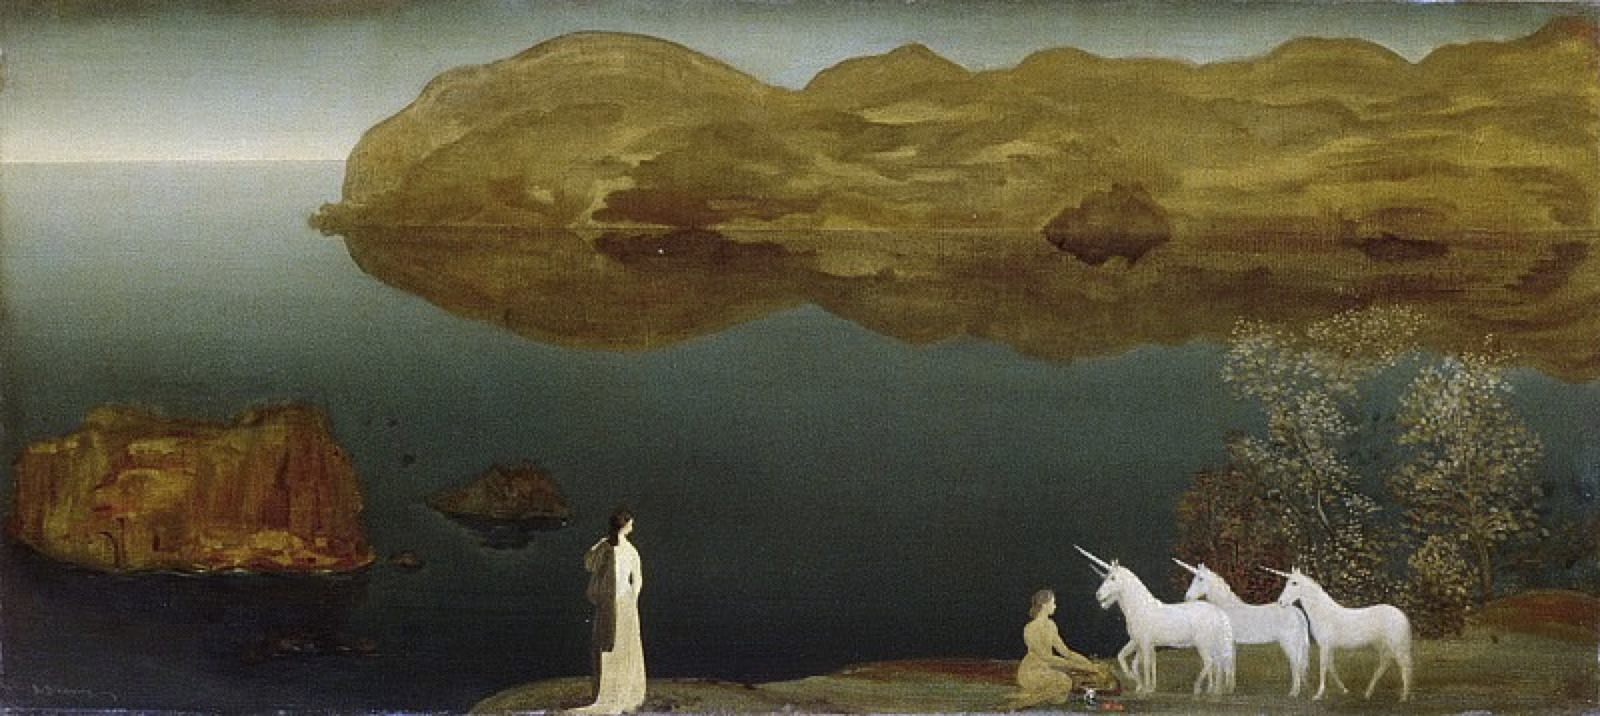
\includegraphics[width=\textwidth,height=0.75\textheight,keepaspectratio]{unicornios.jpg}
      {\footnotesize\color{gray}[Arthur B. Davies - Unicorns (Legend—Sea Calm).]}
  \column{0.57\textwidth}
    \begin{cita}
    Oh, esta es la criatura que nunca existió.\\ 
    No lo sabían; sin importarles, amaron\\
    su gracia, su paso y la forma en que se erguía\\
    mirándolos con ojos claros y calmos.
    \end{cita}
    {\footnotesize\color{gray}[Rainer Maria Rilke, \emph{Sonetos a Orfeo}, II.4]}
  \end{columns}

\end{frame}

%\begin{frame}{Rainer Maria Rilke, \emph{Sonetos a Orfeo}, II.4}
%  \begin{columns}[T]
%  \column{0.48\textwidth}
%    \begin{cita}
%    O dieses ist das Tier, das es nicht giebt.\\
%    Sie wußtens nicht und habens jeden Falls\\
%    -- sein Wandeln, seine Haltung, seinen Hals,\\
%    bis in des stillen Blickes Licht -- geliebt.
%    \end{cita}
%  \column{0.48\textwidth}
%    \begin{cita}
%    Oh, este es el animal que no existe.\\
%    Ellos no lo sabían, y en todo caso amaron\\
%    -- su andar, su porte, su cuello,\\
%    hasta la luz de su mirada serena.
%    \end{cita}
%    {\footnotesize\color{gray}[Traducción provisional. Definitiva: JJGC.]}
%  \end{columns}
%\end{frame}

%\begin{frame}
%  \frase{¿Para qué sirven los unicornios?}
%\end{frame}

% =====================================================================
% 1. UNICORNIO 1: EL NEUTRINO
% =====================================================================
% --- T3 antigua (2026-09-14): sustituida por las tres siguientes ---
%\begin{frame}{Desintegración beta}
%  \begin{columns}
%  \column{0.4\textwidth}
%    
\includegraphics[width=\textwidth,height=0.70\textheight,keepaspectratio]{betaDecay.jpg}
%    
%   ${}^3_1\mathrm{H}\ (\text{tritio}) \rightarrow {}^3_2\mathrm{He}\ (\text{helio-3})$
%  \column{0.6\textwidth}
%  $\bullet$~A principios del siglo XX, los físicos estudiaban el fenómeno de la radioactividad, descubierto por Henri Becquerel en 1896 y estudiado por Marie y Pierre Curie.
%  
%  $\bullet$~En la llamada \emph{desintegración beta}, un isótopo radioactivo se desintegraba a otro más ligero emitiendo una partícula beta (un electrón).
%  
%  $\bullet$~\emph{¡La energía de esa partícula beta debería ser siempre la misma!}, $E_\beta = \Delta M \cdot c^2$, 
%  donde $\Delta M = M_{{}^3_1\mathrm{H}} - M_{{}^3_2\mathrm{He}}$ es la diferencia de masas entre los isótopos padre e hijo. 
%  
%  %$\bullet$~Si medimos muchas veces la energía del beta, esperamos encontrar las medidas en un rango muy estrecho (una línea para un detector perfecto).
%  
% 
%  \end{columns}
%\end{frame}

\begin{frame}{Radiactividad}
  \begin{columns}
  \column{0.45\textwidth}
    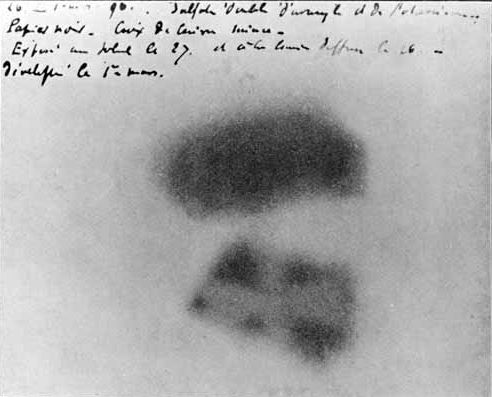
\includegraphics[width=\textwidth,height=0.72\textheight,keepaspectratio]{becquerelPlate.jpg}

    {\footnotesize\color{gray}Placa fotográfica de Henri Becquerel, 1896.}
  \column{0.55\textwidth}
    $\bullet$~En 1896, Becquerel guarda unas sales de uranio sobre una placa fotográfica envuelta en papel negro. La placa se vela: algo invisible sale del uranio y atraviesa el papel.

    $\bullet$~Marie y Pierre Curie llaman \emph{radiactividad} al fenómeno. Se trata de una extraña propiedad de la naturaleza que hace que algunos átomos no sean estables sino que se desintegren a otros más ligeros emitiendo   \emph{radiación}.
  \end{columns}
\end{frame}

\begin{frame}{Desintegración beta}
  \begin{columns}[T]
  \column{0.45\textwidth}
    \begin{center}
    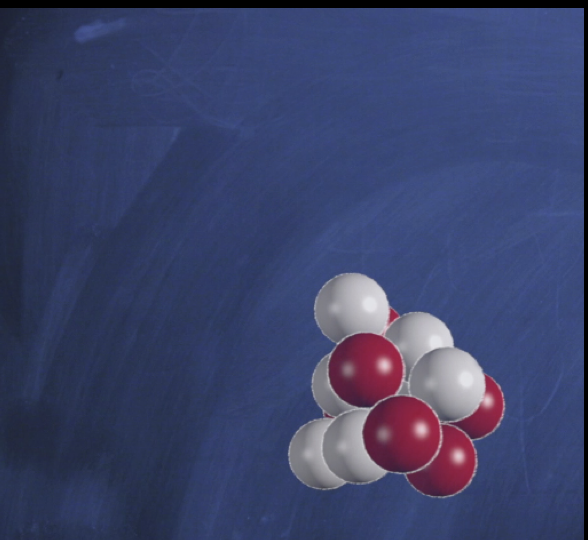
\includegraphics[width=\textwidth,height=0.45\textheight,keepaspectratio]{c14.png}\\
    {\color{uwopurple}\textbf{Carbono-14}}
    \end{center}
  \column{0.1\textwidth}
    \vspace{0.22\textheight}
    \begin{center}{\Huge\color{uwopurple}$\rightarrow$}\end{center}
  \column{0.45\textwidth}
    \begin{center}
    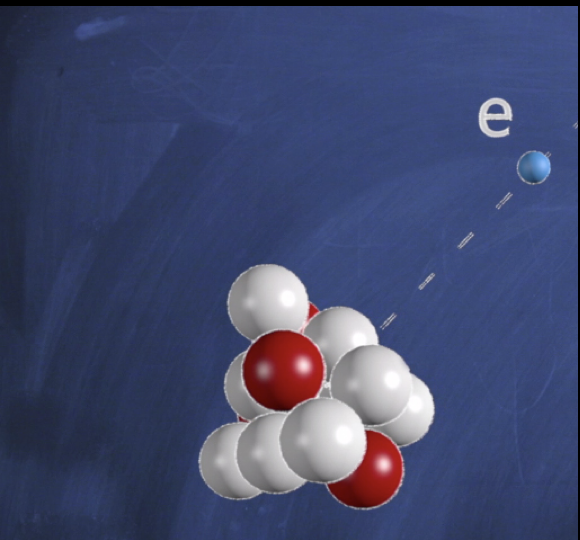
\includegraphics[width=\textwidth,height=0.45\textheight,keepaspectratio]{n14.png}\\
    {\color{uwopurple}\textbf{Nitrógeno-14 + electrón}}
    \end{center}
  \end{columns}
  \vspace{1ex}
  $\bullet$~En la \emph{desintegración beta}, un núcleo radiactivo se transforma en otro emitiendo una <<partícula beta>> (el nombre histórico con que se denominaron los electrones).  En el ejemplo, el Carbono-14 (6 protones y 8 neutrones) se transforma en N-14 (7 protones y 7 neutrones), emitiendo un electrón. 
\end{frame}

\begin{frame}{La energía del electrón}
  \begin{columns}
  \column{0.5\textwidth}
    \begin{tikzpicture}
      \node[anchor=south west,inner sep=0] (img) {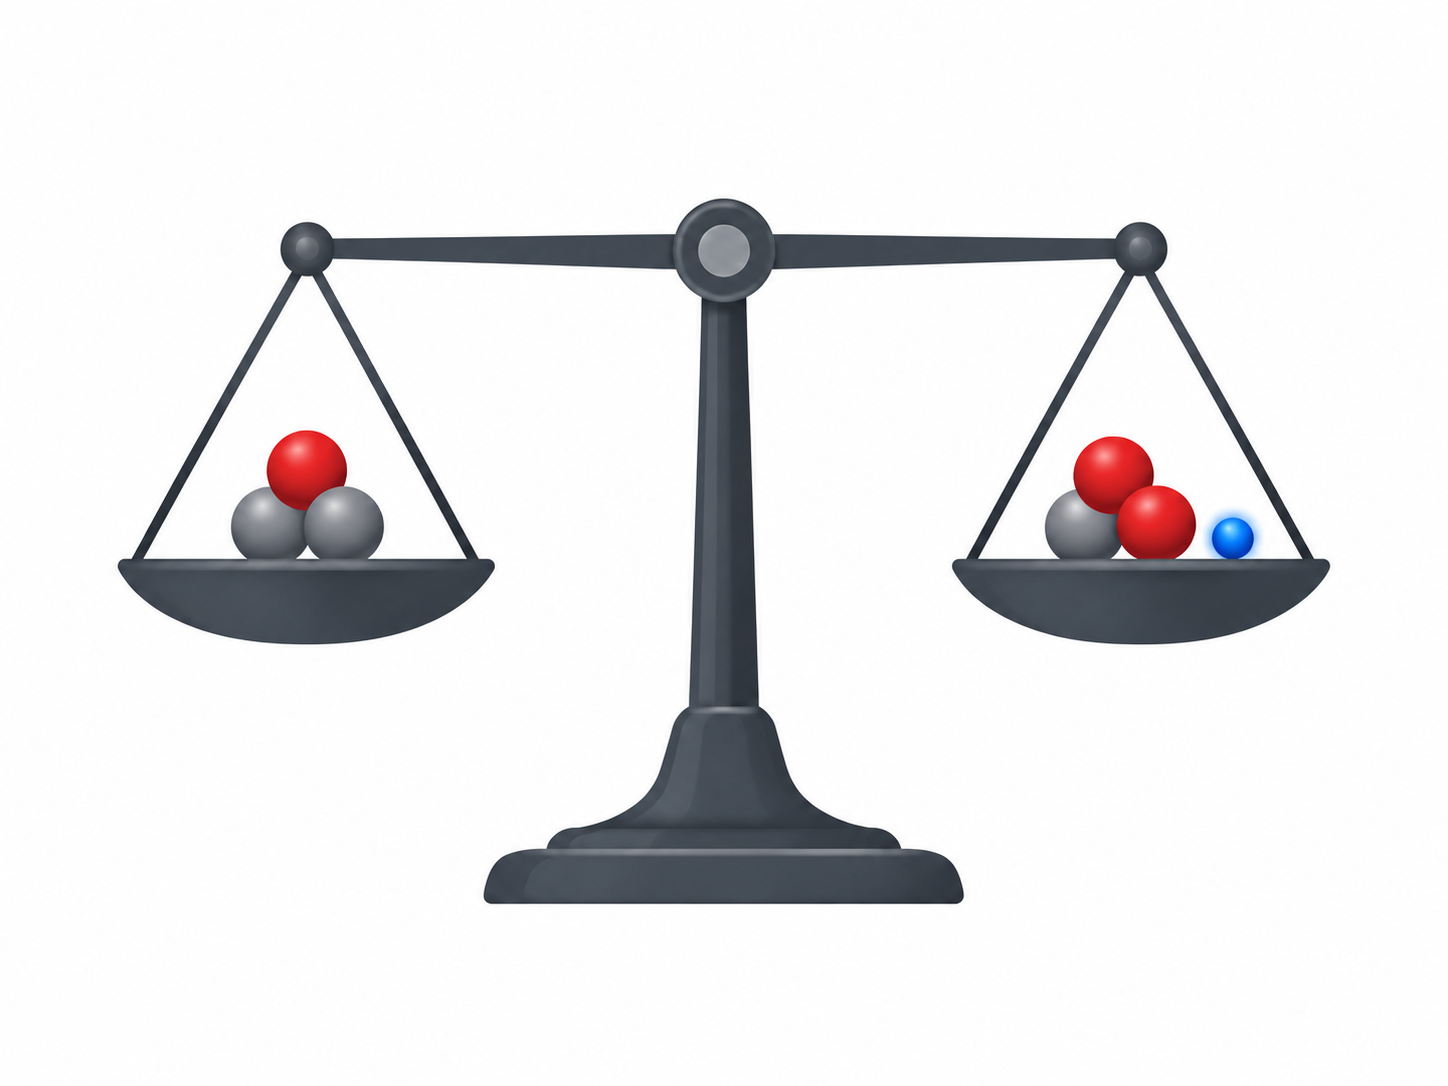
\includegraphics[width=\textwidth]{balance2.png}};
      \begin{scope}[x={(img.south east)},y={(img.north west)}]
       % \node[color=uwopurple,font=\small\bfseries] at (0.21,0.20) {tritio};
        %\node[color=uwopurple,font=\small\bfseries] at (0.78,0.40) {helio-3};
       % \node[color=uwopurple,font=\small\bfseries] at (0.93,0.80) {electrón};
      \end{scope}
    \end{tikzpicture}
  \column{0.5\textwidth}
  
    $\bullet$~En el ejemplo un núcleo de Tritio (2 neutrones y un protón) se convierte en un núcleo de Helio-3 (dos protones y un neutrón) y se emite un electrón.
    
    $\bullet$~La masa del núcleo padre tiene que ser igual a la del hijo más la del electrón que se emite.

    $\bullet$~Por lo tanto la energía del electrón es siempre la diferencia de masas entre el padre y el hijo. 

    $\bullet$~Como la diferencia de masas es siempre la misma, \emph{el electrón debería emitirse siempre con la misma energía}.
  \end{columns}
\end{frame}


\begin{frame}{La energía del electrón debería ser siempre la misma}
  \begin{center}
  \begin{tikzpicture}[scale=0.85]
    \onslide<1->{\fila{4.6}{1}}
    \onslide<2->{\fila{2.4}{2}}
    \onslide<3->{\node at (2.85,2.05) {$\vdots$}; \node at (7.6,2.05) {$\vdots$}; \fila{0}{12}}
  \end{tikzpicture}
  \end{center}
%  \vspace{-1ex}
 % $\bullet$~Si medimos muchos electrones, todos deberían tener la misma energía.
\end{frame}

\begin{frame}{Pero cada electrón tenía una energía diferente}
  \begin{center}
  \begin{tikzpicture}[scale=0.85]
    \onslide<1->{\filae{4.6}{6.2/1}}
    \onslide<2->{\filae{2.4}{5.8/1,7.0/1}}
    \onslide<3->{\node at (2.85,2.05) {$\vdots$}; \node at (7.6,2.05) {$\vdots$};
                 \filae{0}{5.6/1,5.8/5,6.0/10,6.2/15,6.4/10,6.6/5,6.8/3,7.0/2,7.2/1}}
  \end{tikzpicture}
  \end{center}
\end{frame}


% --- T6 antigua 'Conservación de la energía' (2026-09-14): sustituida ---
\begin{frame}{Conservación de la energía}
  \begin{columns}
  \column{0.55\textwidth}
    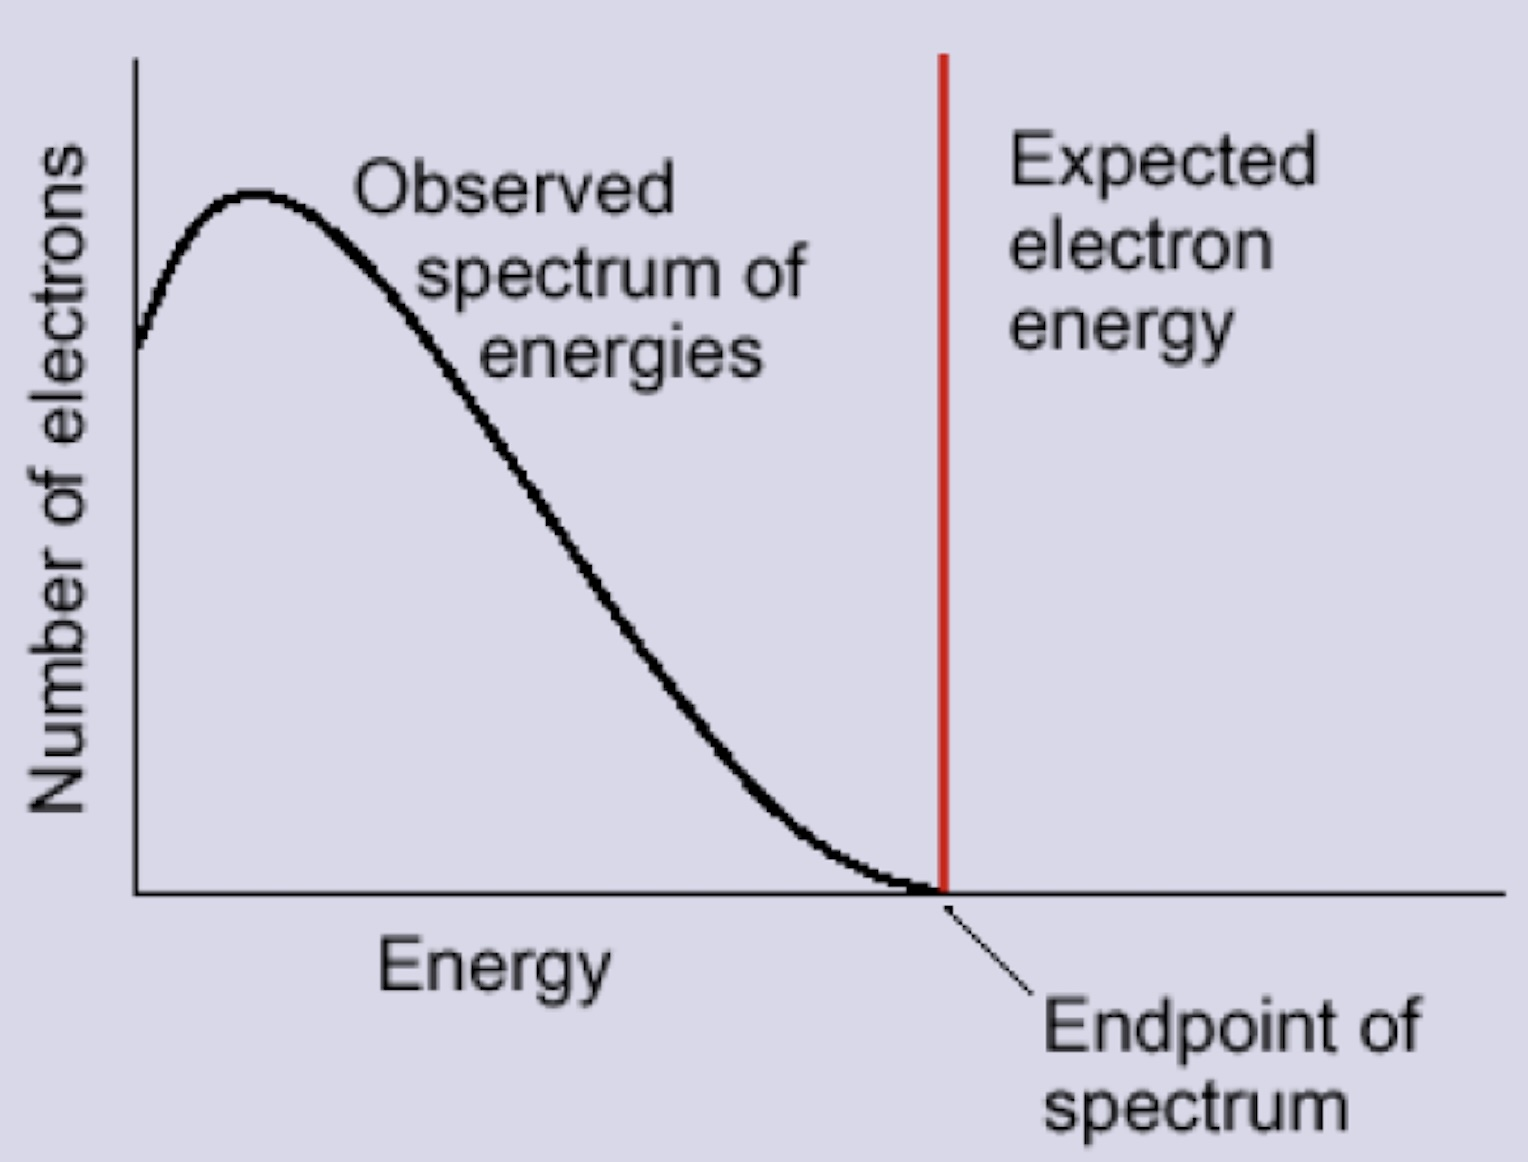
\includegraphics[width=\textwidth,height=0.70\textheight,keepaspectratio]{betaSpectrum.jpg}
    
  \column{0.45\textwidth}
  
   
  $\bullet$~En lugar de una línea estrecha situada en $Q_\beta = \Delta M \cdot c^2$, los físicos observaban que los electrones podían tener cualquier energía sin llegar nunca a $Q_\beta$. ¿Dónde se iba la energía que les faltaba a los electrones? 
  
  $\bullet$~¿Era posible que la energía no se conservara en la desintegración beta? \emph{¡Anathema sit!, ¡Contra primum principium!, ¡Energia non conservatur, absit!}
  \end{columns}
\end{frame}

%\begin{frame}{La conservación de la energía es sagrada}
%  \begin{columns}
%  \column{0.5\textwidth}
%    \pendiente[0.55\textheight]{Grabado de un móvil perpetuo (dominio público).}
%  \column{0.5\textwidth}
%    Si la energía no se conservase, se podría construir una máquina de
%    movimiento perpetuo.\\[1ex]
%    Nadie lo ha conseguido nunca.\\[1ex]
%    Para un físico, la conservación de la energía es lo mismo que decir que
%    las leyes de la naturaleza son las mismas hoy que mañana.
%  \end{columns}
%\end{frame}

\begin{frame}{Un remedio desesperado}
  \begin{columns}
  \column{0.5\textwidth}
    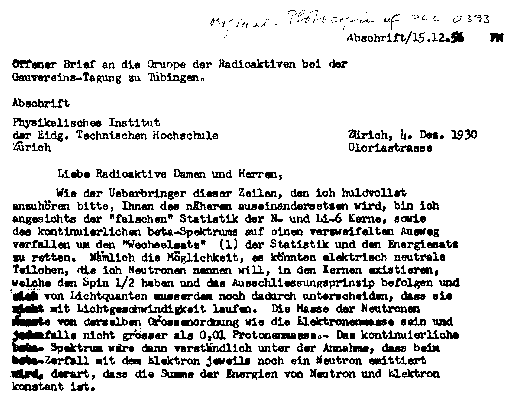
\includegraphics[width=\textwidth]{liebe.png}
  \column{0.5\textwidth}
    \begin{cita}
    Queridas y radioactivas damas y caballeros: [\dots] a causa del espectro beta
    continuo, he dado con un \emph{remedio desesperado} para salvar la ley de
    conservación de la energía.
    \end{cita}
    %Una partícula invisible, sin carga, que se lleva la energía que falta.
  \end{columns}
\end{frame}


\begin{frame}{¿Por qué desesperado?}
\begin{columns}
\column{0.50\textwidth}

\includegraphics[scale=0.65]{desperate.png}

\column{0.50\textwidth}
 $\bullet$~{\bf Porque la conservación de la energía implica que la física no depende de traslaciones espacio-temporales}. En otras palabras, los físicos creen que las leyes de la naturaleza deben ser las mismas aquí y en Andrómeda y las mismas hoy, el año que viene y hace un millón de años. 

\end{columns}

\end{frame}

\begin{frame}{¿Cuál era el remedio?}
\begin{columns}
\column{0.50\textwidth}

\includegraphics[scale=0.35]{betadecaywithnu.png}
   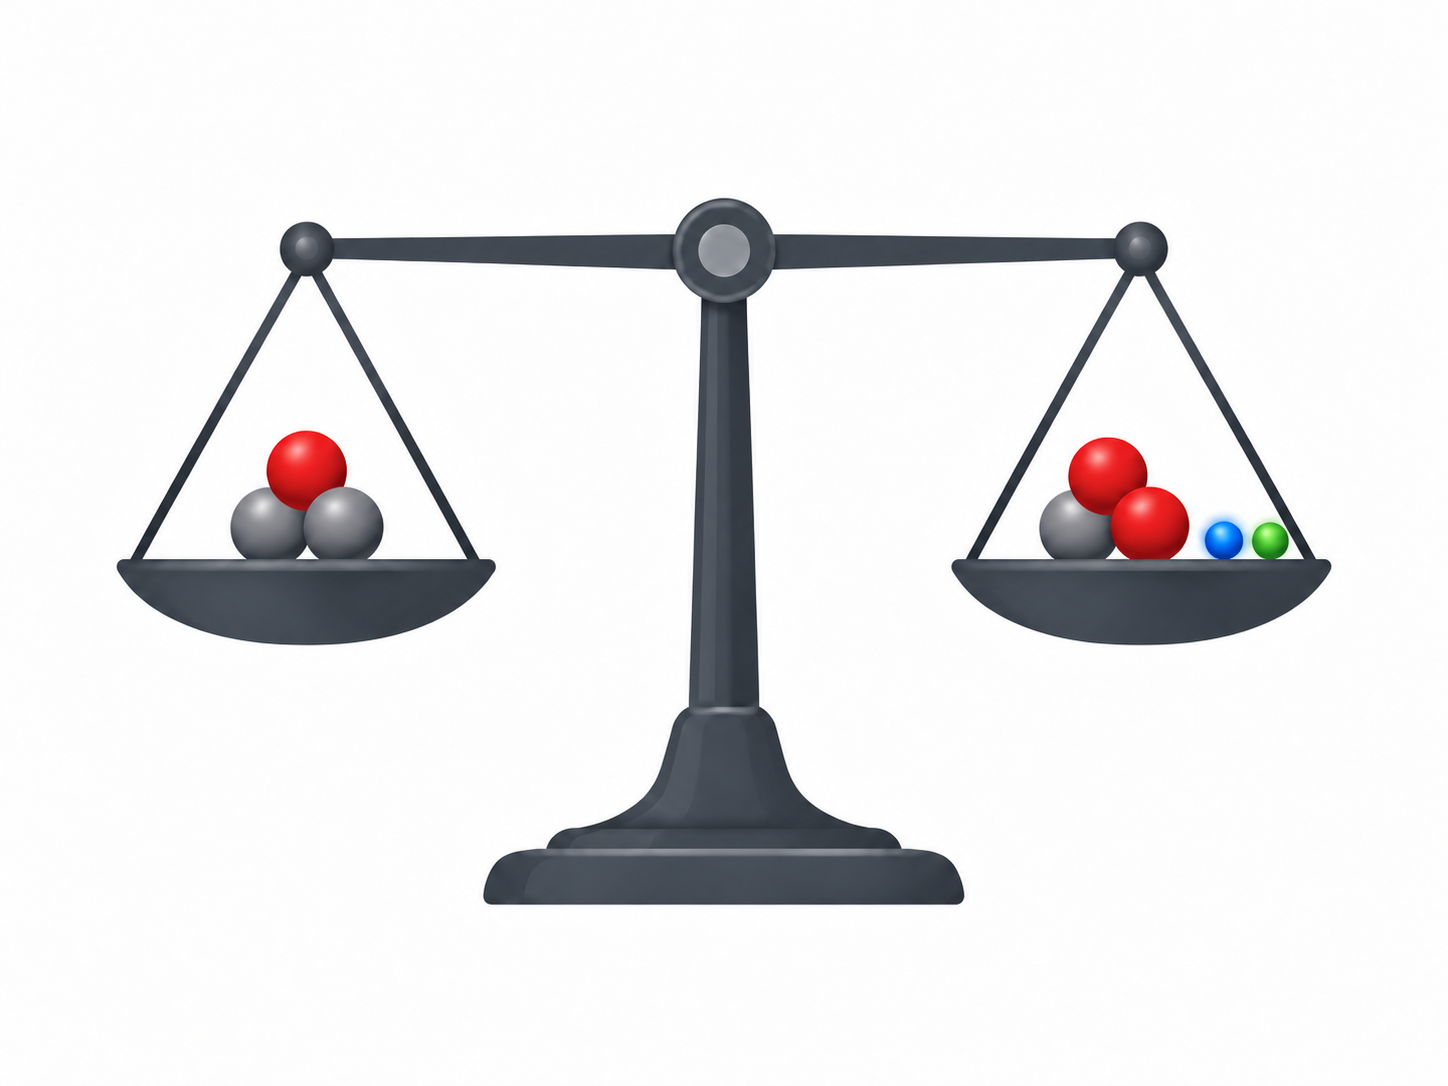
\includegraphics[width=\textwidth,height=0.45\textheight,keepaspectratio]{balance3.png}
\column{0.50\textwidth}
 $\bullet$~Pauli propuso introducir una segunda partícula que se emitía en la desintegración beta junto con el electrón, pero se escapaba sin ser detectada. 
 
  $\bullet$~Esta partícula (que Pauli bautizó como neutrón y más tarde Fermi rebautizaría como neutrino, o pequeño neutrón) no puede tener carga eléctrica, su masa es muy ligera o nula y no puede interaccionar (casi) con la materia, ya que los detectores no la registraban. 
  
   $\bullet$~En otras palabras, Pauli había propuesto introducir un unicornio (una criatura inexistente, pero bellísima) en un proceso de física. 
   

\end{columns}

\end{frame}

\begin{frame}{Desnudar a un santo para vestir a otro}
  \begin{columns}
  \column{0.5\textwidth}
    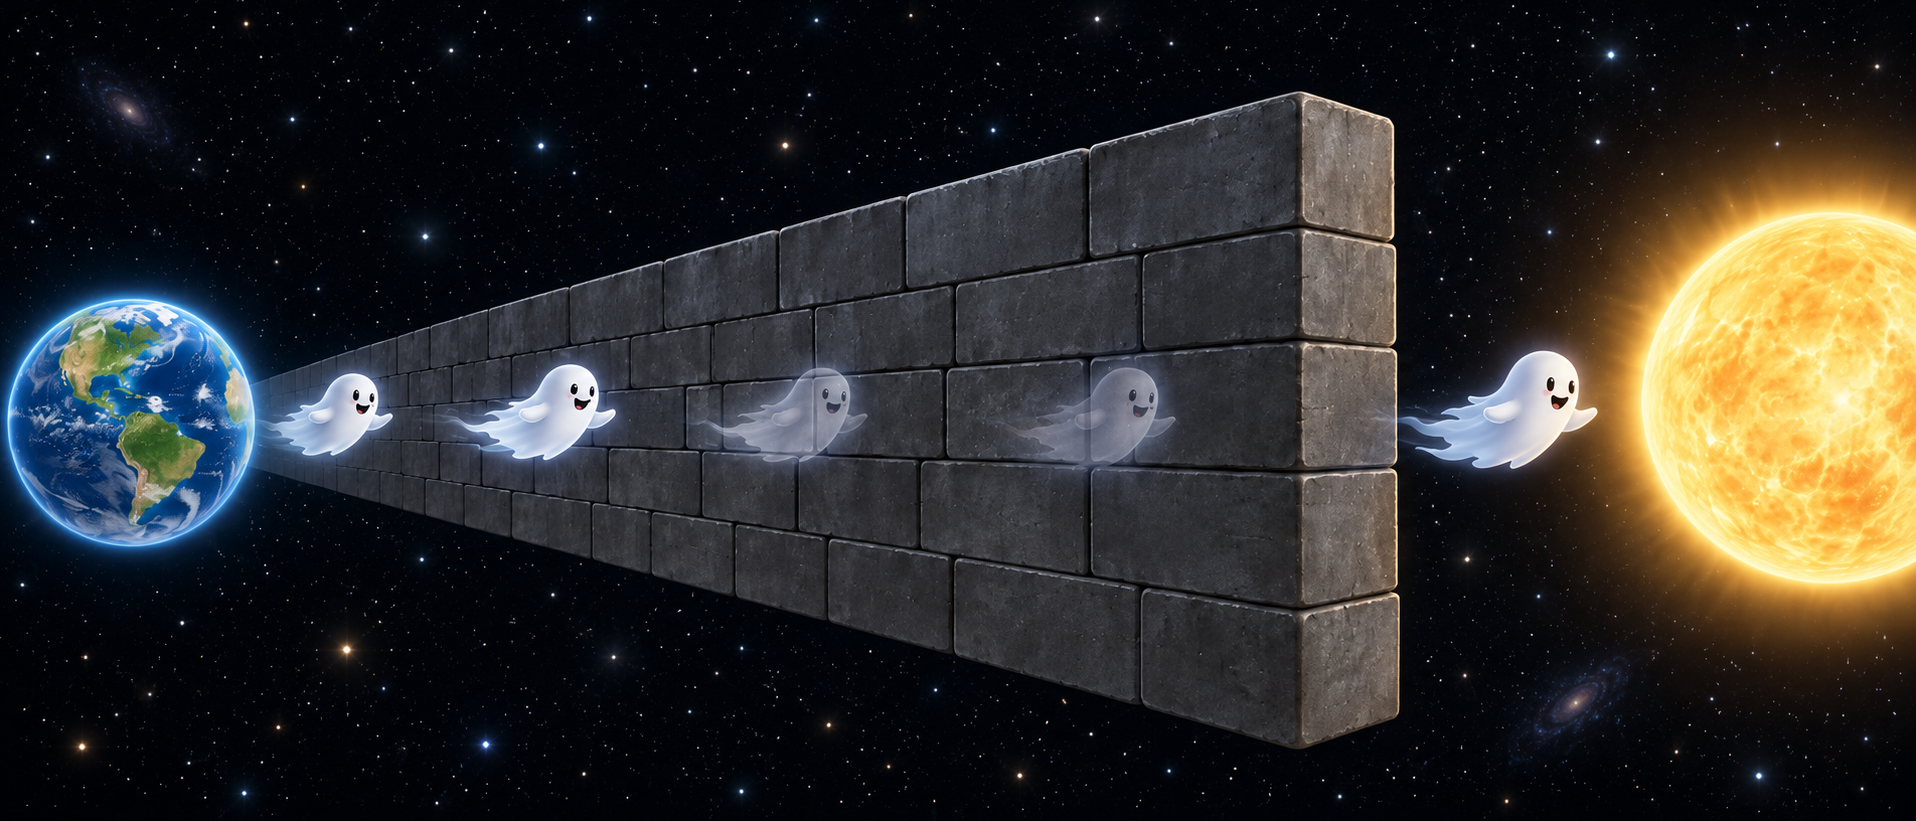
\includegraphics[width=\textwidth,height=0.75\textheight,keepaspectratio]{ghosts.png}
    
     $\bullet$~El neutrino resuelve el problema de la conservación de la energía a cambio de introducir una partícula que (aparentemente) no puede detectarse.
  \column{0.5\textwidth}
 
  
  $\bullet$~De hecho, la probabilidad de que un neutrino individual interaccione con la materia ordinaria es tan baja, que el neutrino emitido en la desintegración beta necesita atravesar {\em cuatro años luz de plomo} (la distancia entre la Tierra y la estrella más cercana, Alfa Centauri) para reaccionar con un átomo. Es decir, la probabilidad de detectar un neutrino individual se aproxima a cero.  
%    \begin{cita}
%    Queridas y radioactivas damas y caballeros: [\dots] a causa del espectro beta
%    continuo, he dado con un \emph{remedio desesperado} para salvar la ley de
%    conservación de la energía.
%    \end{cita}
%    %Una partícula invisible, sin carga, que se lleva la energía que falta.
  \end{columns}
\end{frame}

%\begin{frame}{``He hecho algo terrible''}
%  \begin{columns}
%  \column{0.35\textwidth}
%    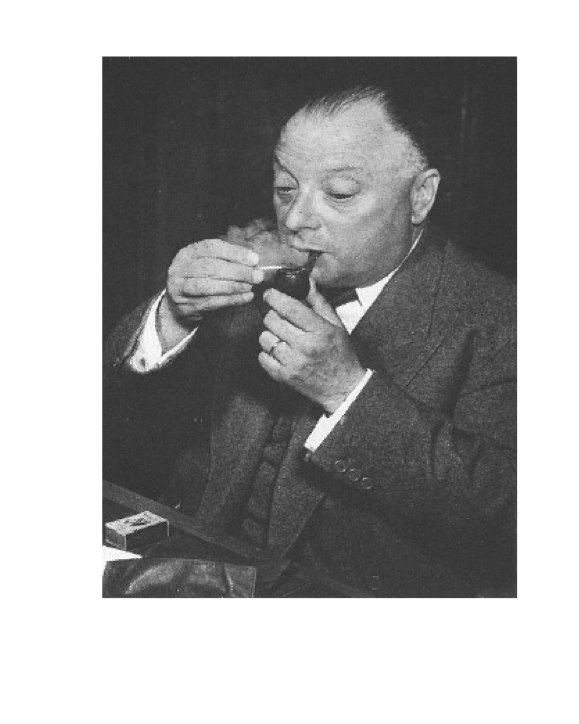
\includegraphics[width=\textwidth]{pauli.png}
%  \column{0.6\textwidth}
%    \begin{cita}
%    He hecho algo terrible: he propuesto una partícula que no puede
%    detectarse. Es algo que ningún teórico debería hacer jamás.
%    \end{cita}
%    \hfill Wolfgang Pauli
%  \end{columns}
%\end{frame}

%\begin{frame}{De neutrón a neutrino}
%  \begin{columns}
%  \column{0.5\textwidth}
%    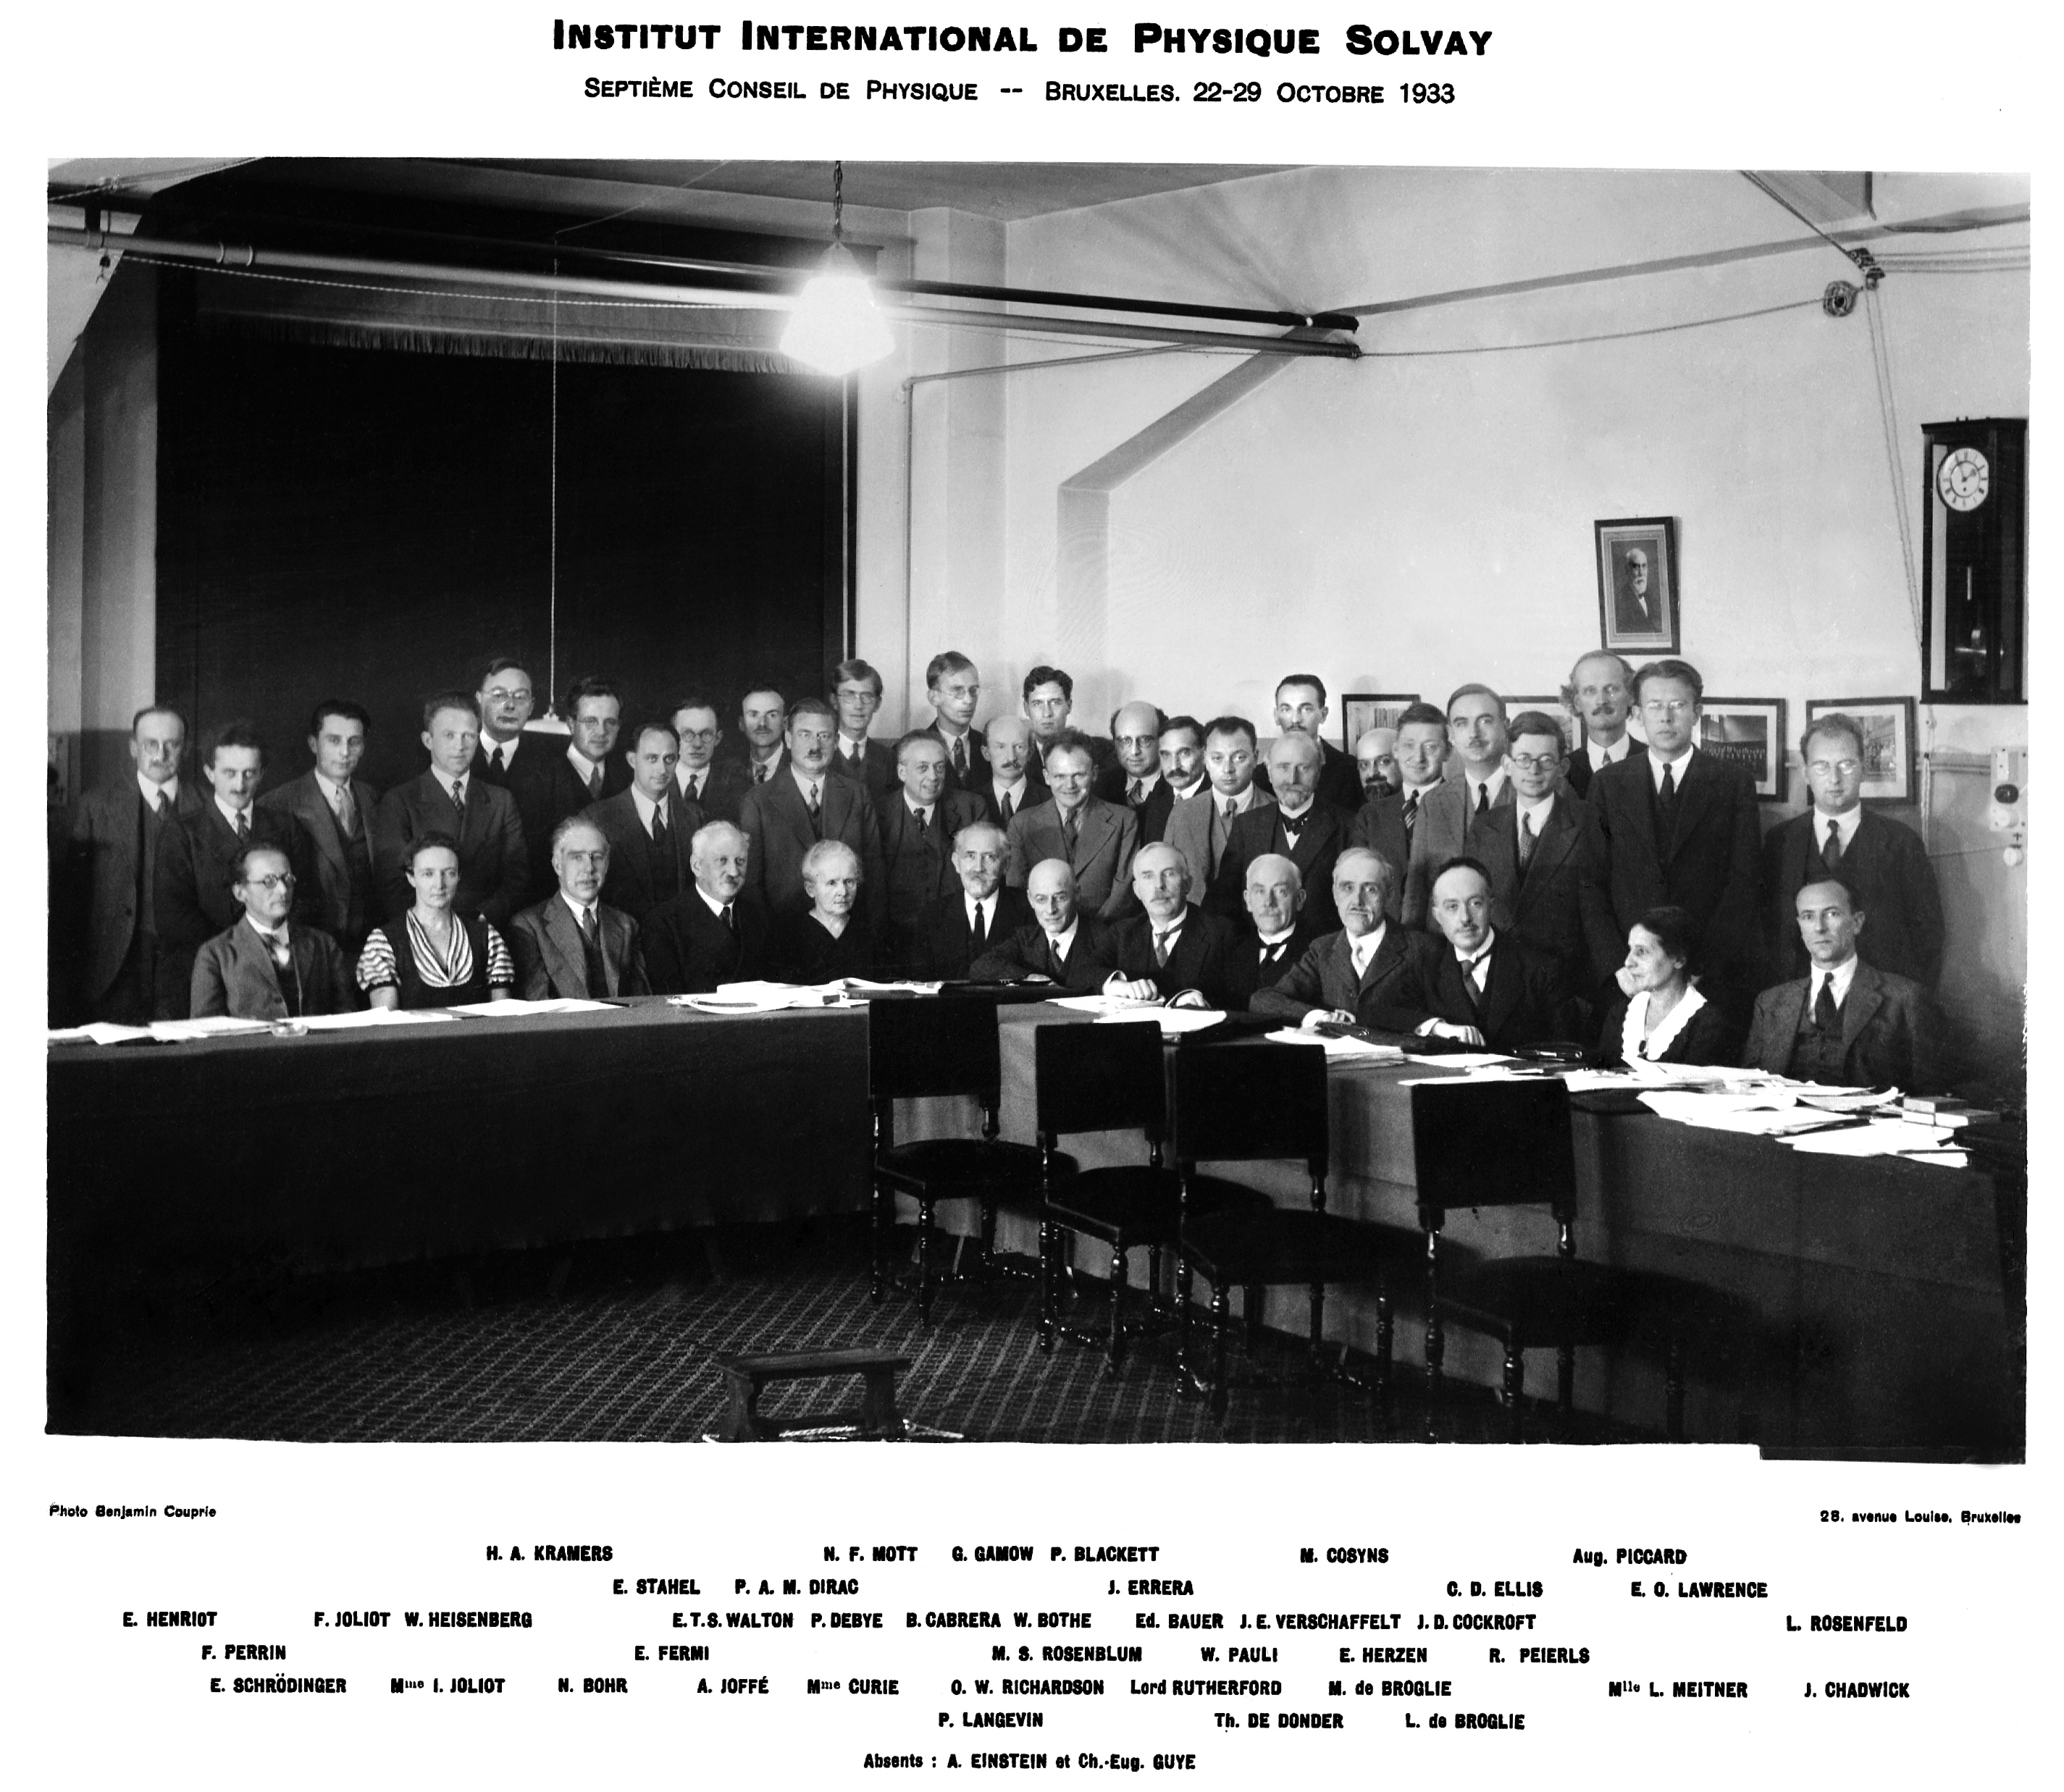
\includegraphics[width=\textwidth]{Solvay1933Large.jpg}
%  \column{0.5\textwidth}
%    Pauli llamó a su partícula ``neutrón''.\\[1ex]
%    En 1932 Chadwick descubre el neutrón de verdad, pesado.\\[1ex]
%    Fermi rebautiza al de Pauli: \textbf{neutrino}, el neutroncito.\\[1ex]
%    Pauli, Solvay 1933: \emph{``No sabemos nada de la interacción de los
%    neutrinos con la materia.''}
%  \end{columns}
%\end{frame}

\begin{frame}{La gente seria no cree en los unicornios}
  \begin{columns}
  \column{0.3\textwidth}
    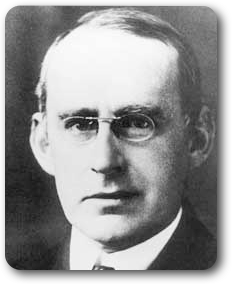
\includegraphics[width=\textwidth]{eddington.png}
  \column{0.68\textwidth}
    \small
    \begin{cita}
    En condiciones normales diría que no creo en los neutrinos\dots\ Pero debo
    recordar que un físico puede ser un artista, y con los artistas nunca se
    sabe; quizá demuestren que mi anticuada incredulidad está fuera de lugar. ¿Me atrevería a afirmar que los
    físicos experimentales no tendrán ingenio suficiente para fabricar
    neutrinos? [\dots] Si lo consiguen y, quién sabe, les encuentran aplicaciones, supongo que tendré que creer en ellos.
    \end{cita}
    \hfill Sir Arthur Eddington, 1935
  \end{columns}
\end{frame}


\begin{frame}{La lotería de Babilonia}
  \begin{columns}
  \column{0.4\textwidth}
     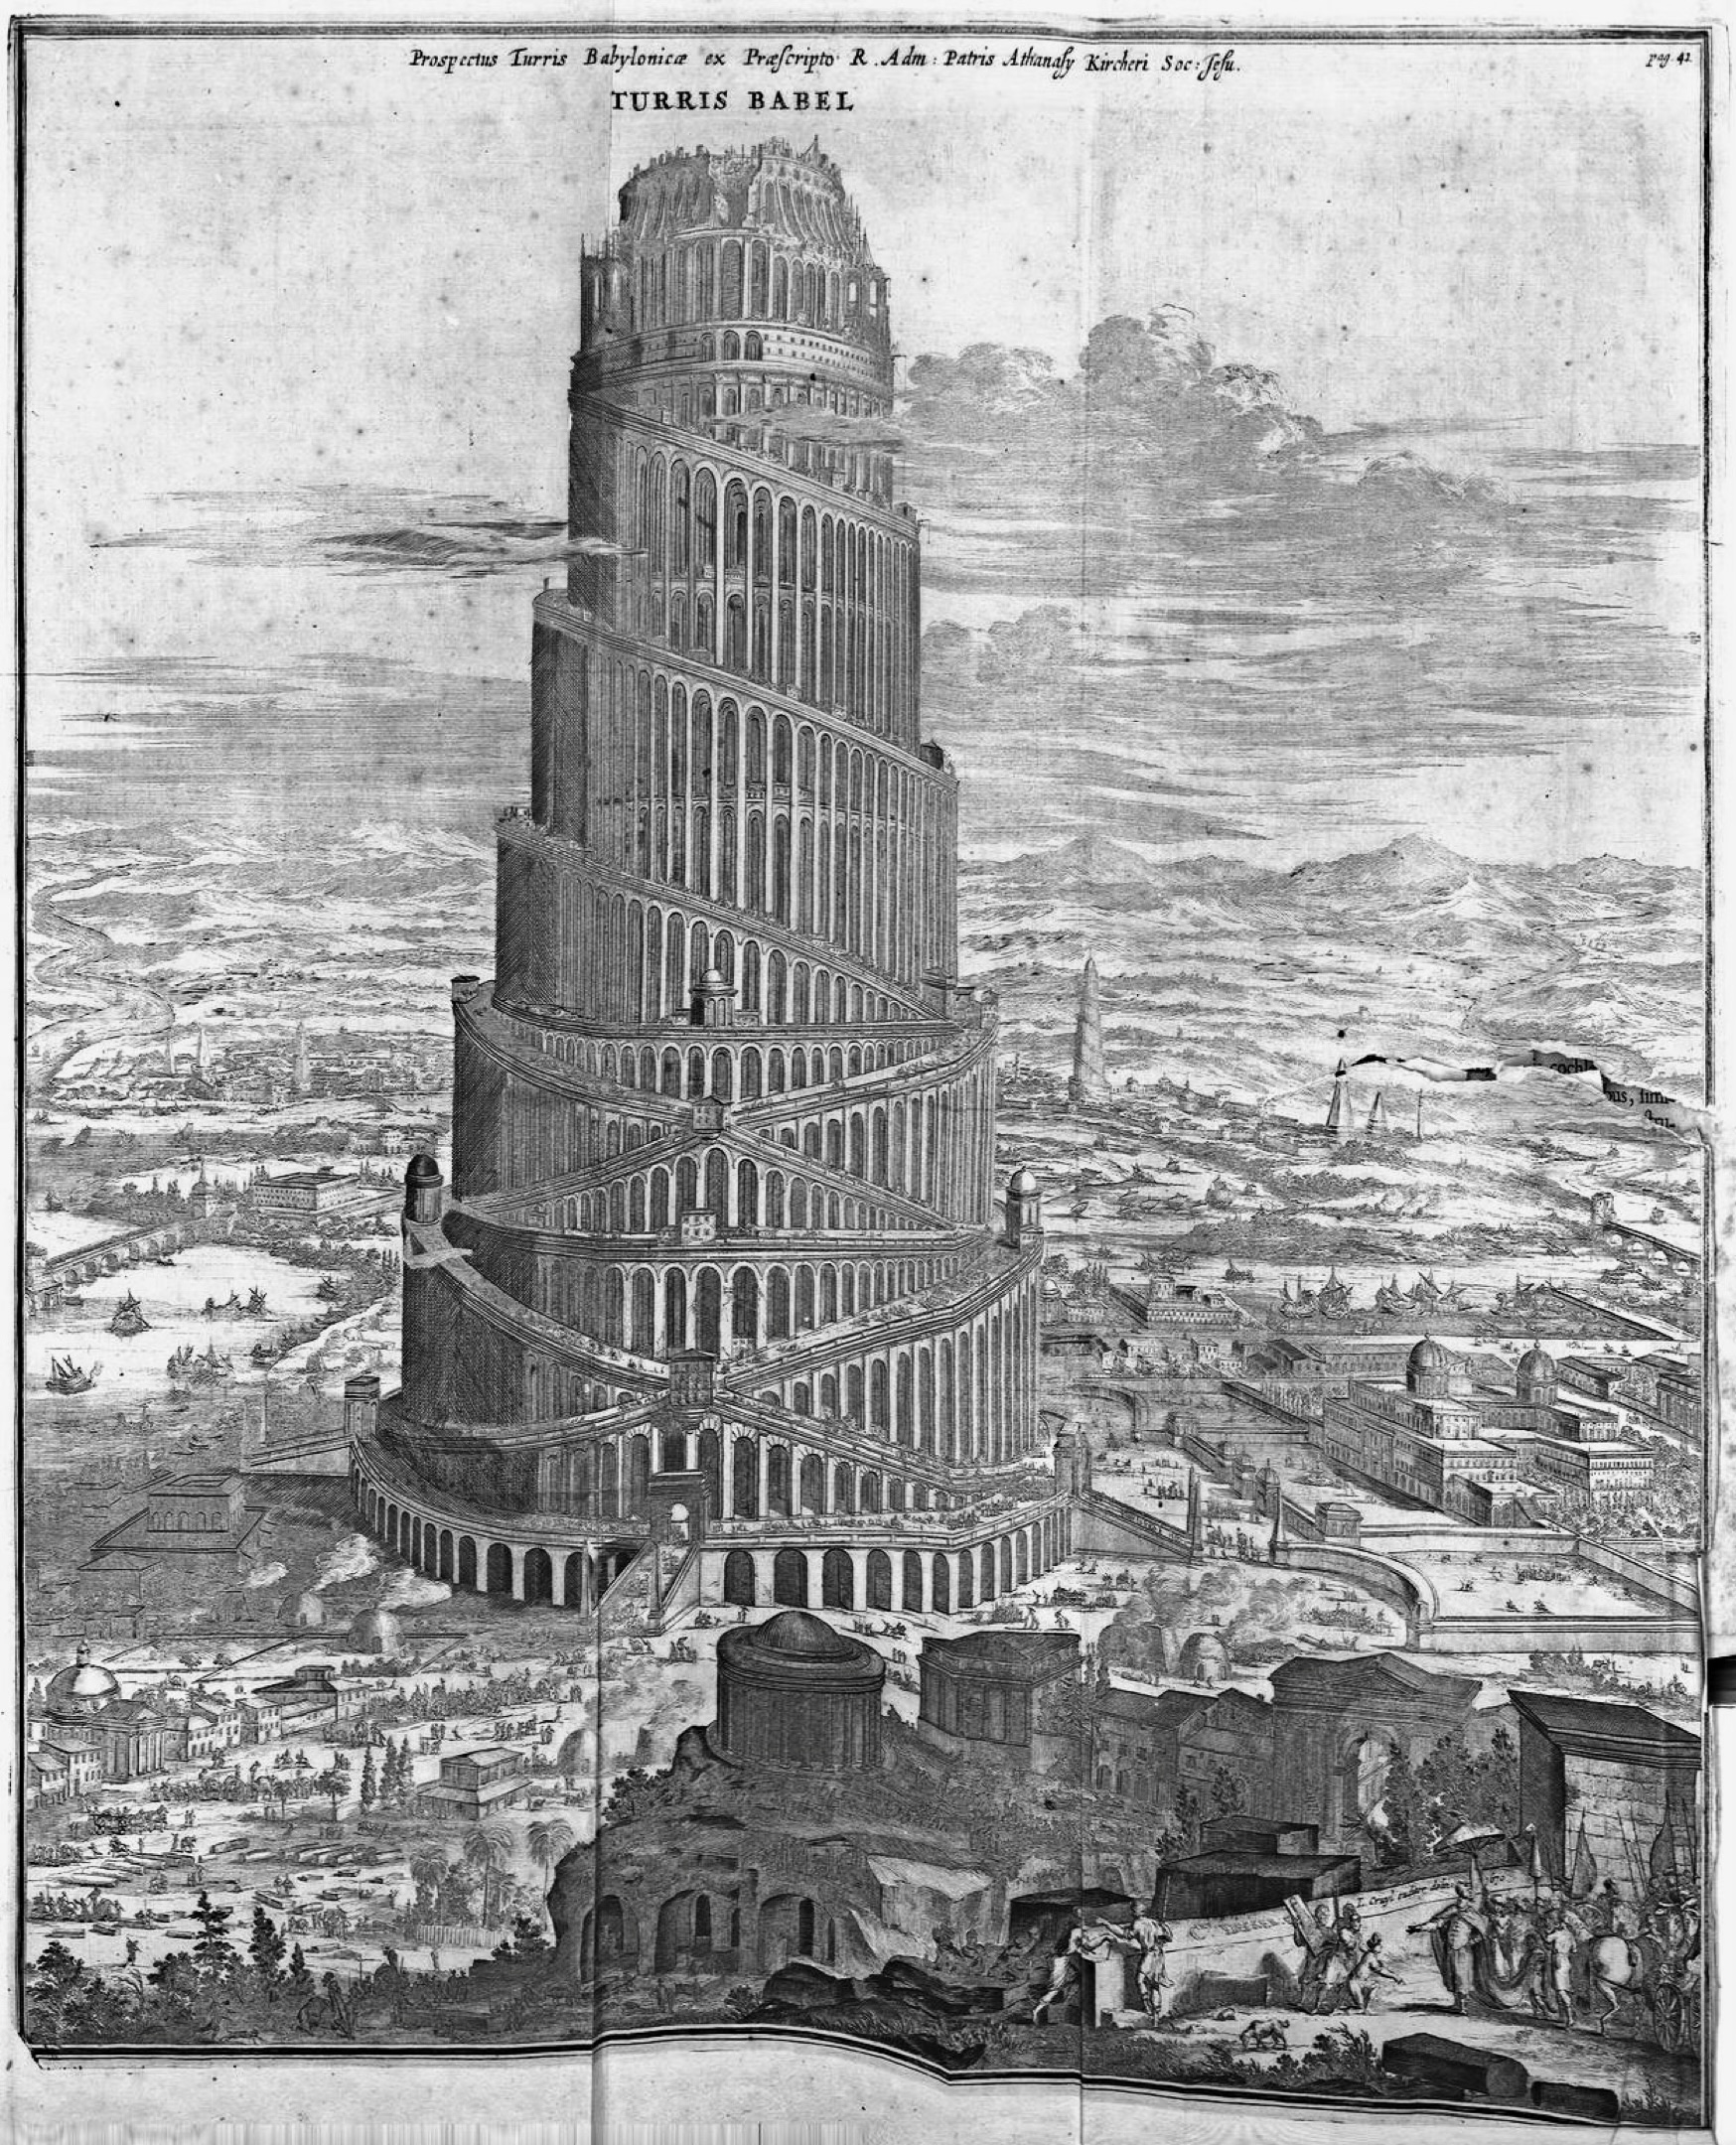
\includegraphics[width=\textwidth]{torrebabel.jpg}
  \column{0.6\textwidth}
  
    $\bullet$~En el célebre relato de J.L. Borges, cualquier ciudadano babilonio puede ser, por un tiempo, cualquier cosa. El narrador ha vivido todas las condiciones humanas posibles debido a los sorteos: ha sido procónsul, esclavo, poseedor de un poder absoluto y prisionero condenado.
    
    $\bullet$~Una forma de interpretar la Lotería es entender que cualquier resultado es posible si se dispone de suficiente tiempo.
    
   $\bullet$~En el caso de los neutrinos, la probabilidad de interacción de cada uno de ellos es pequeñísima, pero algunas fuentes de neutrinos los producen en cantidades gigantescas. Aquí la Lotería consiste en multiplicar ambos números y obtener un resultado positivo, es decir, una interacción. {\em Es posible detectar (muchos) neutrinos siempre que se disponga de una fuente lo bastante intensa}. 
  \end{columns}
\end{frame}


\begin{frame}{Una playa entre Donosti y Moscú}
  \begin{columns}
  \column{0.4\textwidth}
     
\includegraphics[width=\textwidth,height=0.75\textheight,keepaspectratio]{reactorNeutrinos.jpg}
  \column{0.6\textwidth}

    $\bullet$~Un reactor nuclear es un infierno radioactivo encerrado en un búnker. Las desintegraciones en su interior producen $\sim 2 \times 10^{20}$  (doscientos trillones) neutrinos por segundo. Si cada neutrino fuera un grano de arena de La Concha, habría que extender la playa desde Donostia hasta Moscú para que cupieran todos.

    $\bullet$~Un cubo de agua de diez metros de lado, situado a unos 50 metros del reactor, registra unas 370.000 interacciones al día. Cada vez que un <<neutrino>> interacciona con el agua se produce un <<electrón>>.
  \end{columns}
\end{frame}


\begin{frame}{Proyecto Poltergeist}
  \begin{columns}
  \column{0.5\textwidth}
     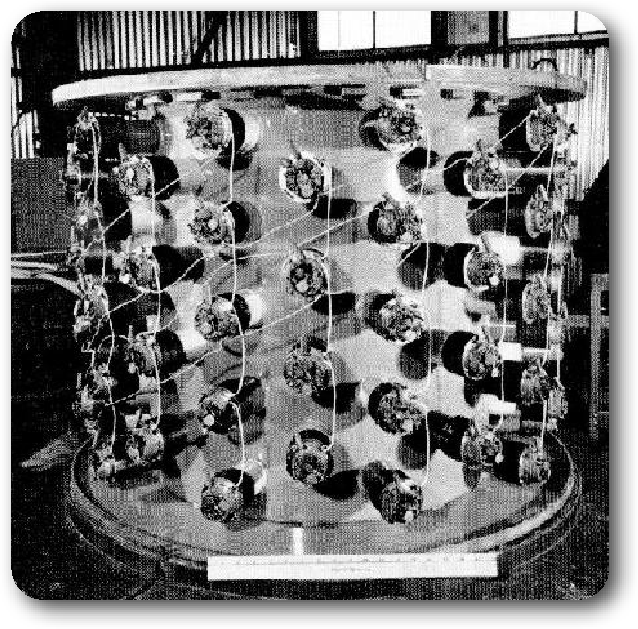
\includegraphics[width=\textwidth,height=0.50\textheight,keepaspectratio]{poltergeist.pdf}
     
      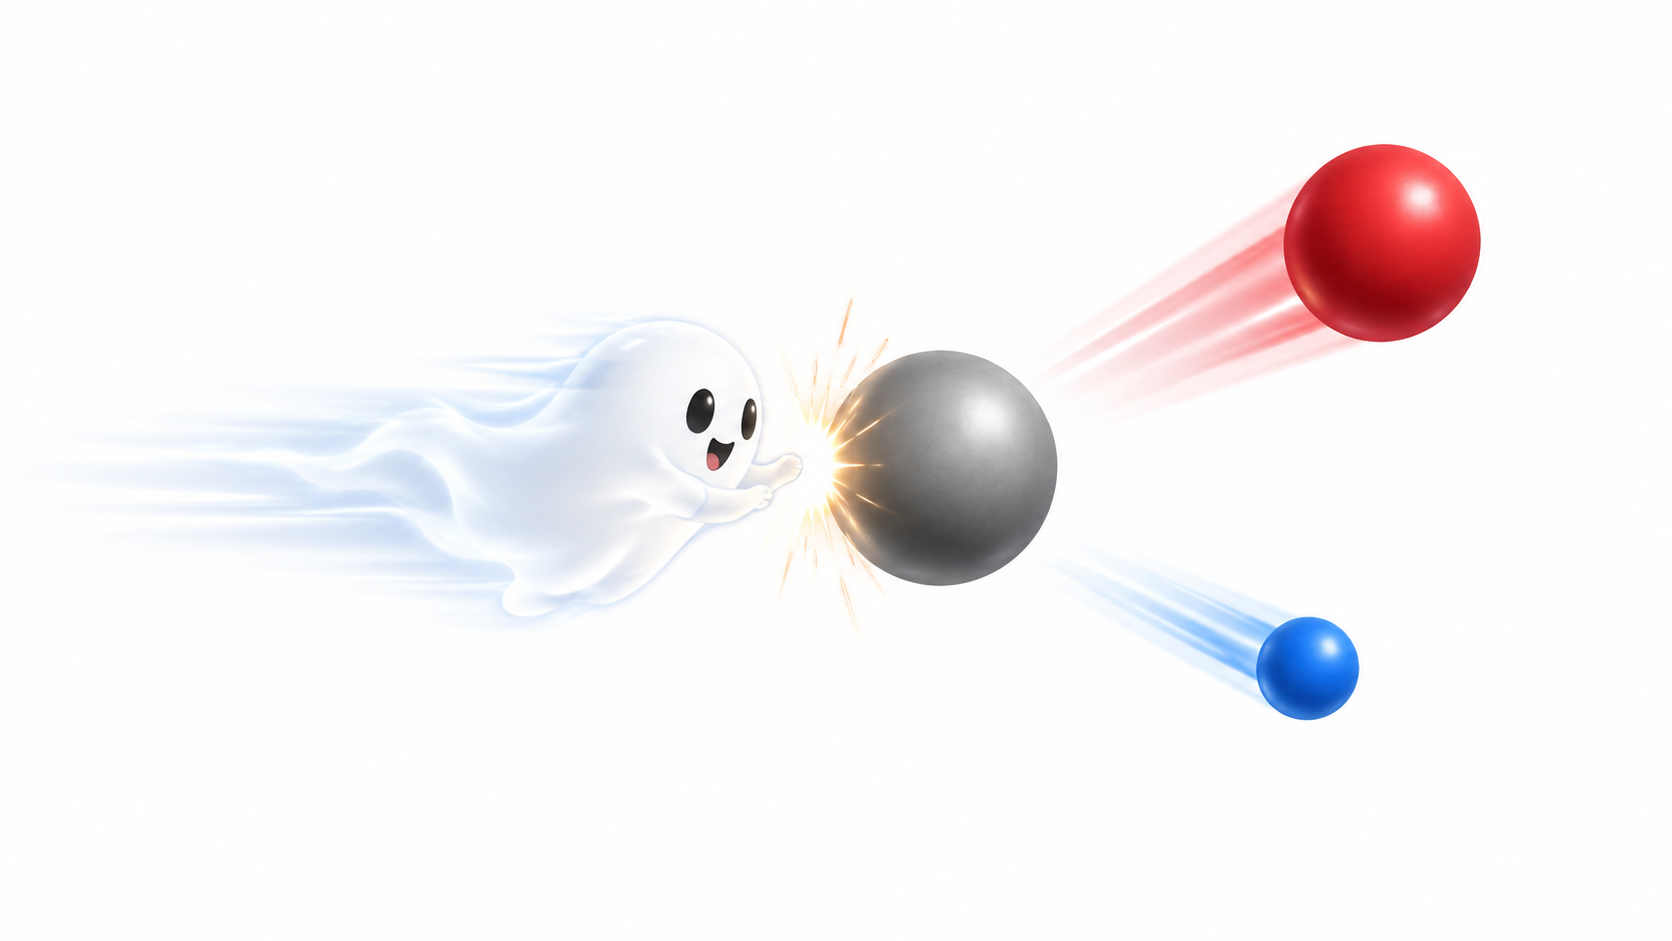
\includegraphics[width=\textwidth,height=0.50\textheight,keepaspectratio]{interaction_nue.png}
     
  \column{0.5\textwidth}
      
   $\bullet$~En 1956, Reines y Cowan jugaron a la lotería de Babilonia y ganaron, registrando <<electrones>> en su detector, producidos por neutrinos del reactor. 
   
    $\bullet$~En realidad un reactor nuclear produce antineutrinos (es decir neutrinos de antimateria) y en la reacción se emiten positrones (es decir electrones de antimateria).  
  \end{columns}
\end{frame}


\begin{frame}{Setenta años más tarde en Vandellós}
  \begin{columns}
  \column{0.5\textwidth}
    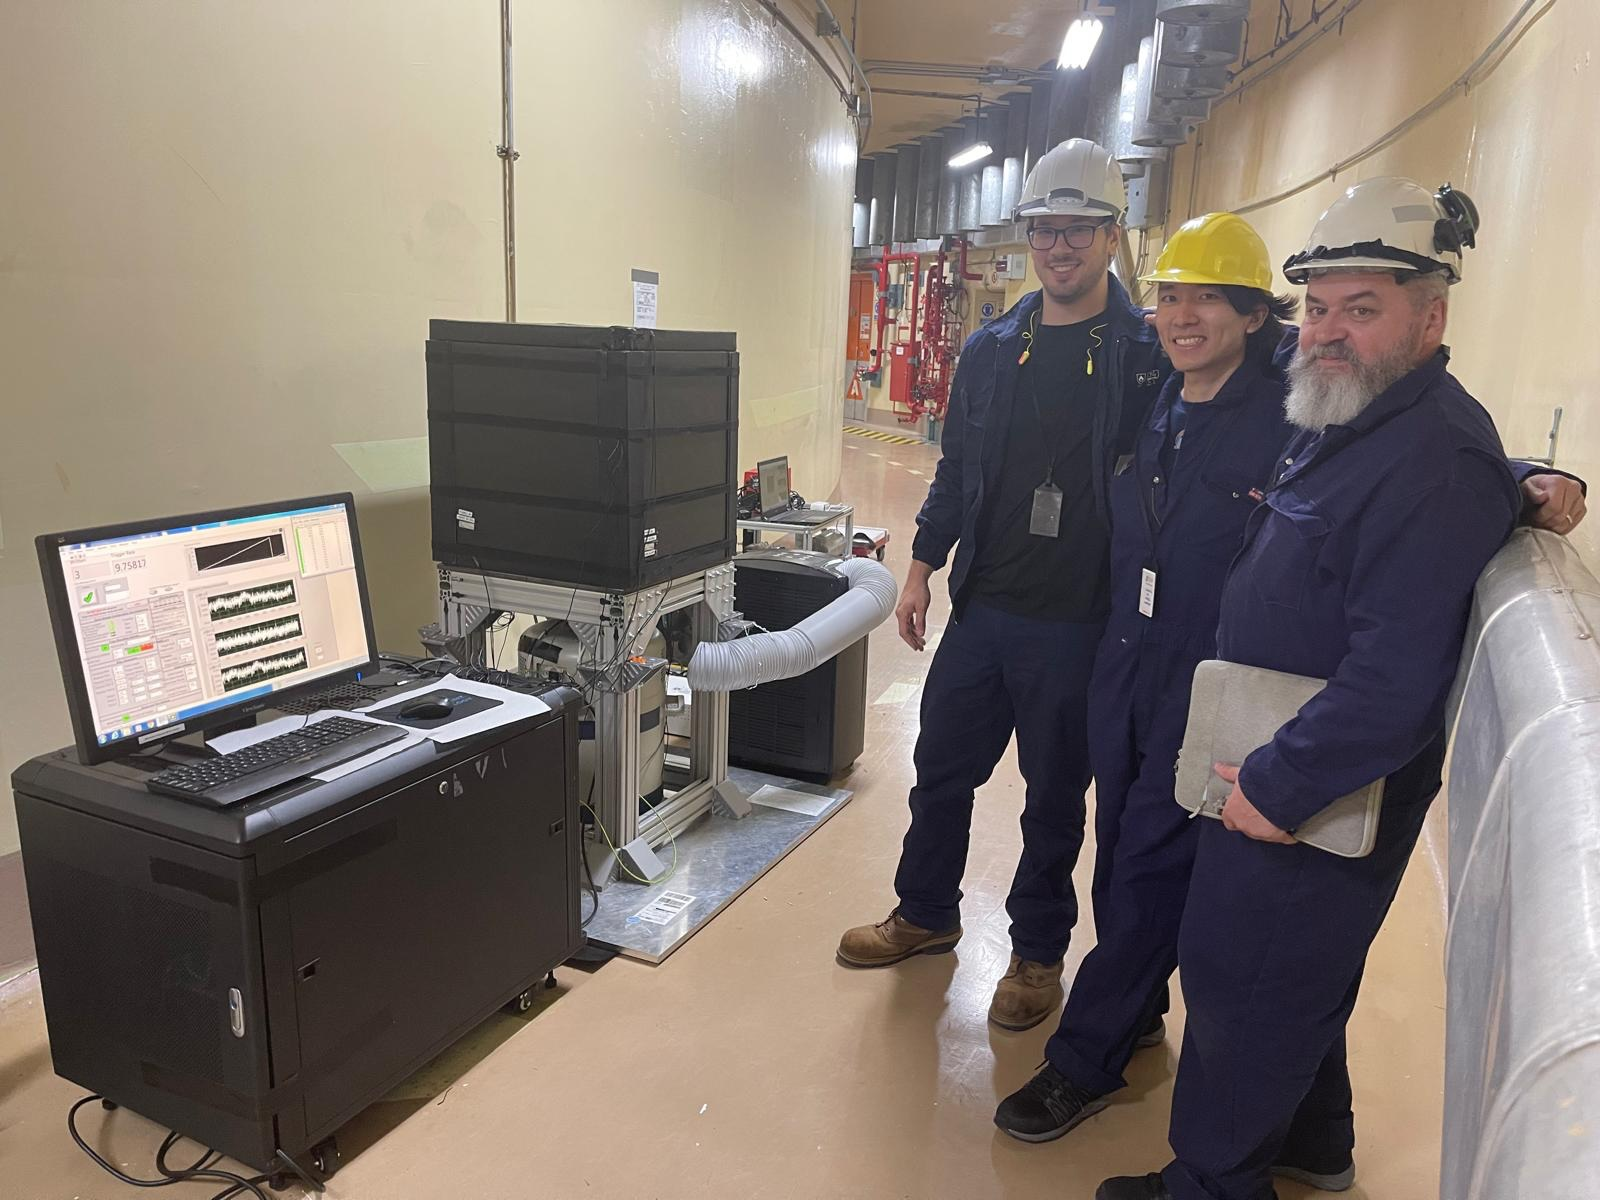
\includegraphics[width=\textwidth,height=0.70\textheight,keepaspectratio]{vandellos2.jpg}
  \column{0.5\textwidth}
      
   $\bullet$~J. Collar y los delincuentes habituales en la central nuclear de Vandellós, donde hemos medido el flujo de (anti) neutrinos durante un año, con un detector que cabe encima de una mesa (único en el mundo). 
   
 
  \end{columns}
\end{frame}

\begin{frame}{El fantasma y la proliferación nuclear}
  \begin{columns}
  \column{0.5\textwidth}
    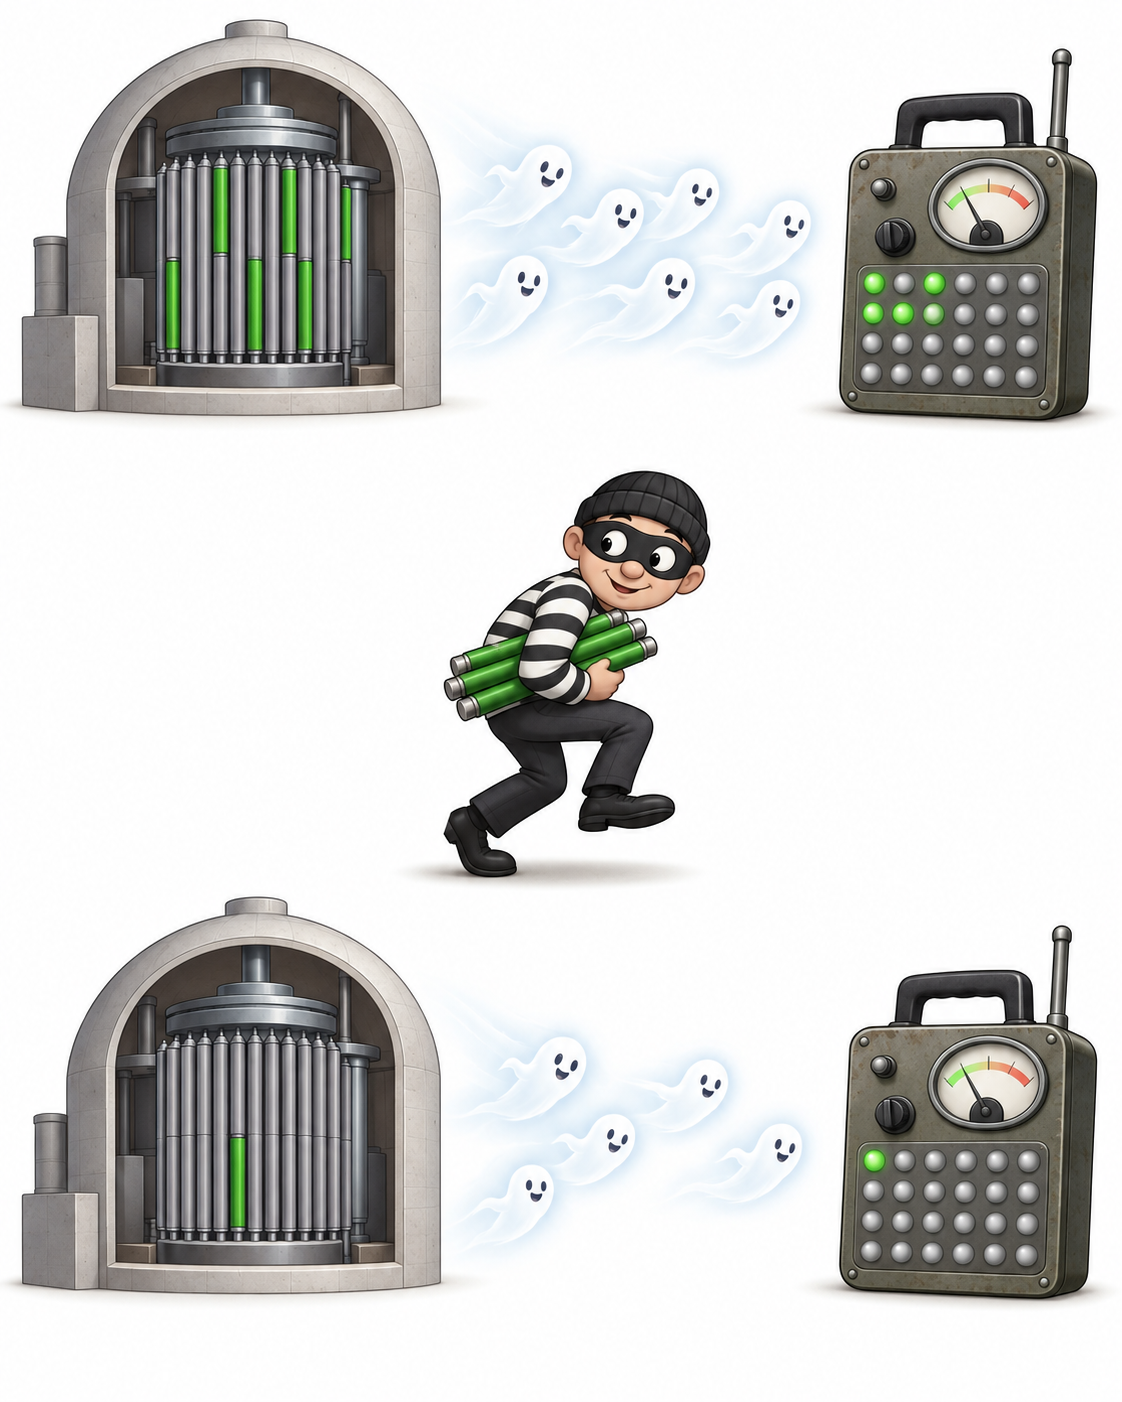
\includegraphics[width=\textwidth,height=0.70\textheight,keepaspectratio]{steelingNeutrinos.png}
  \column{0.5\textwidth}
      
   $\bullet$~En un reactor nuclear se consume uranio y se produce plutonio, un material que puede utilizarse para construir una bomba atómica (con solo unos pocos kilos). 
   
    $\bullet$~Algunos países (India, por ejemplo) se aprovecharon de un programa nuclear civil para <<robar>> el plutonio que necesitaban para fabricar bombas atómicas y convertirse en una potencia nuclear. Hay siempre el riesgo de que se repita la maniobra.
  
   $\bullet$~Pero los neutrinos miden cuánto plutonio hay en el interior del reactor y pueden detectar al ladrón. Así que detectar fantasmas (o unicornios) resulta muy útil para controlar la proliferación nuclear.   
     
  \end{columns}
\end{frame}


\begin{frame}{Neutrinos solares}
  \begin{columns}
  \column{0.4\textwidth}
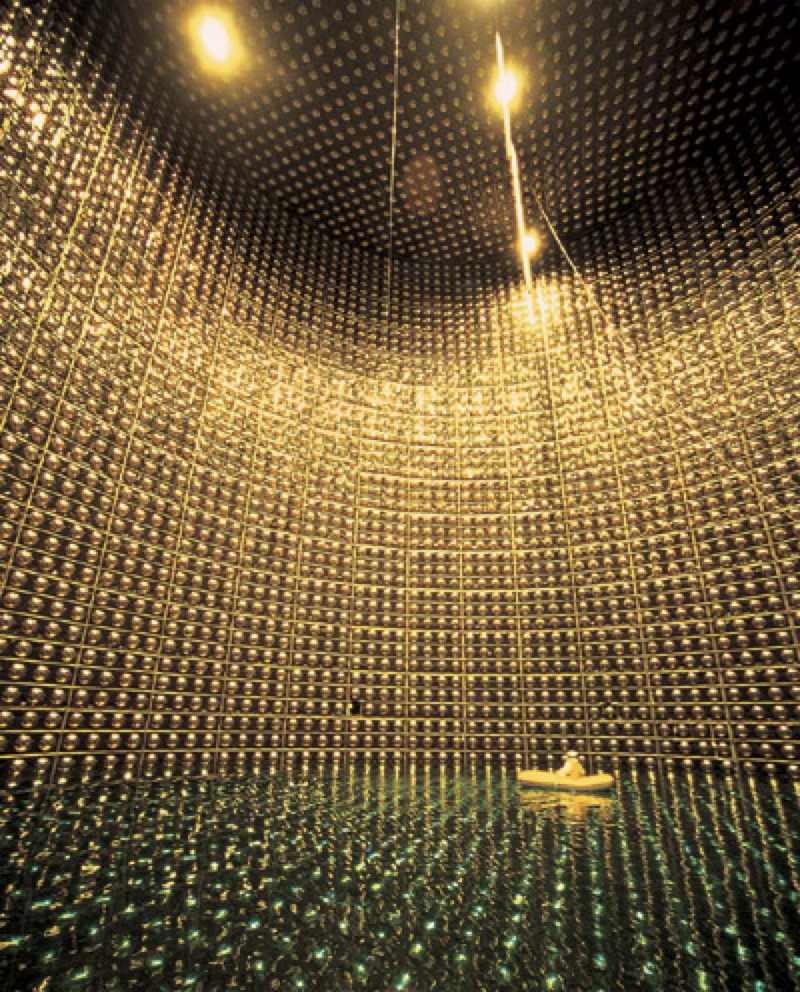
\includegraphics[width=\textwidth,height=0.9\textheight,keepaspectratio]{SK.png}

 \column{0.6\textwidth}
 
 
\includegraphics[width=\textwidth,height=0.40\textheight,keepaspectratio]{neutrinosun.png}

      
   $\bullet$~El Sol es un gigantesco reactor de fusión. A pesar de estar muy lejos de la Tierra, el flujo de neutrinos que nos atraviesa la mano cada segundo es de unos seis billones. Los físicos de neutrinos hemos construido detectores gigantes (Super-Kamiokande y pronto Hyper-Kamiokande, ambos en Japón) para medir estos neutrinos solares y hemos sido capaces de hacer <<neutrinografías>> del Sol. 
  \end{columns}
\end{frame}


\begin{frame}{Paisaje con neutrinos}
  \begin{columns}
  \column{0.5\textwidth}
   $\bullet$~ Paisaje con comanches
   
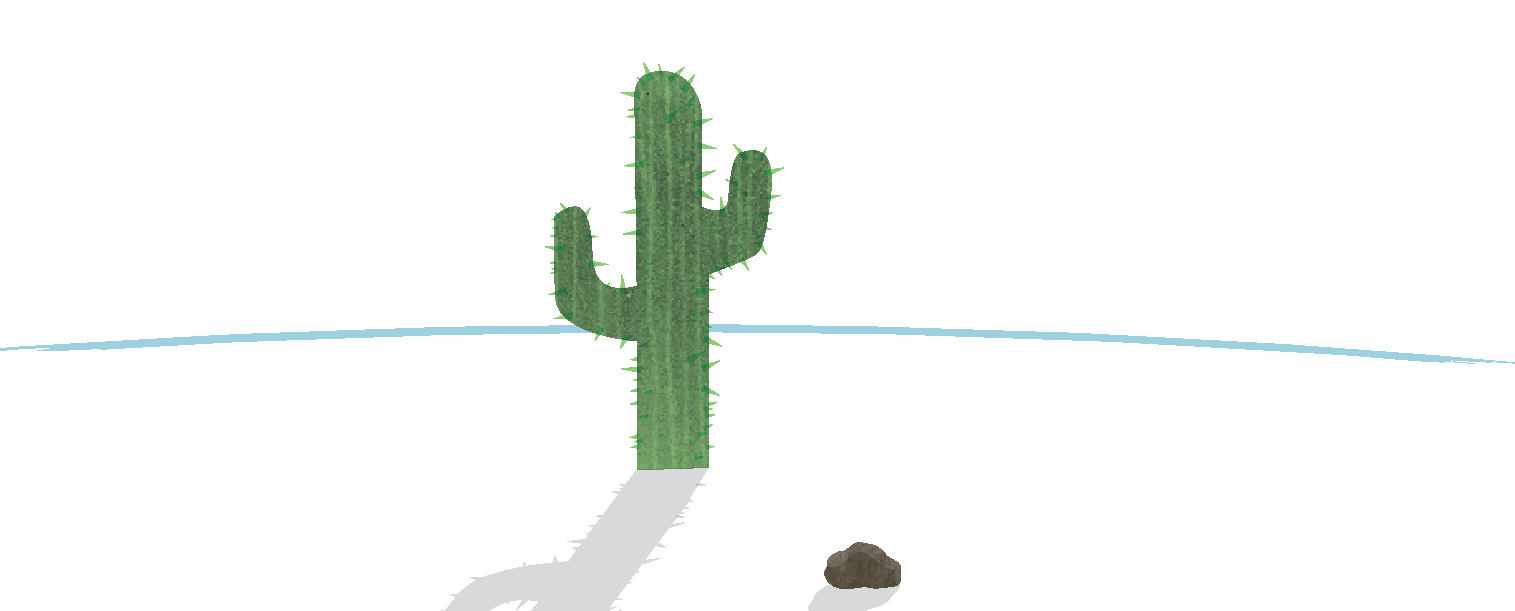
\includegraphics[width=\textwidth,height=0.70\textheight,keepaspectratio]{comanches.pdf}

 \column{0.5\textwidth}
 
  $\bullet$~ Paisaje con neutrinos
  
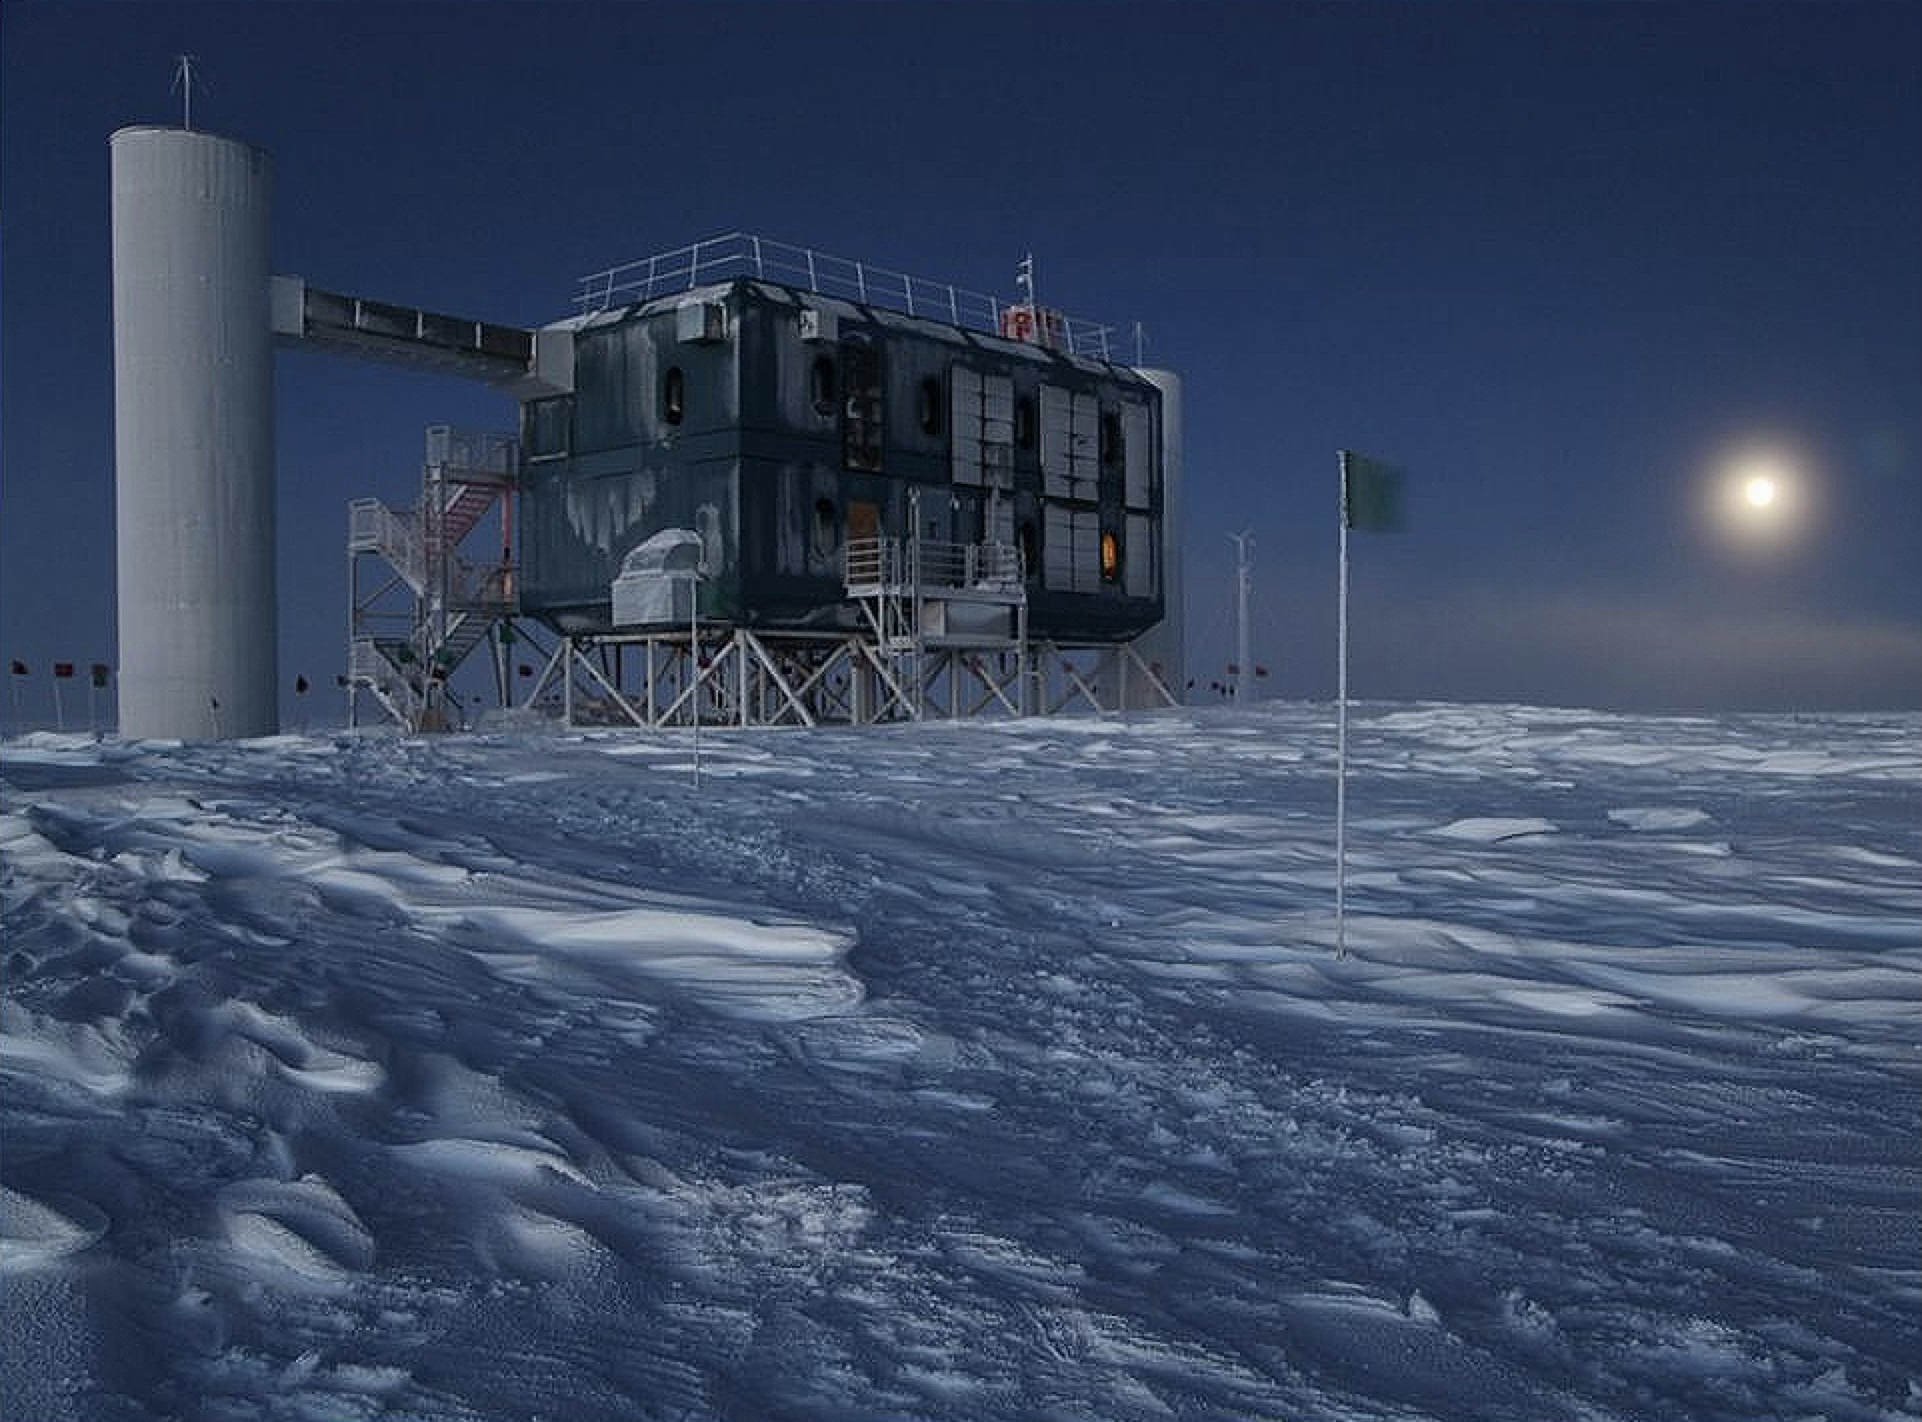
\includegraphics[width=\textwidth,height=0.70\textheight,keepaspectratio]{icecubeout.png}

  \end{columns}
\end{frame}

\begin{frame}{IceCube}
  \begin{columns}
  \column{0.5\textwidth}
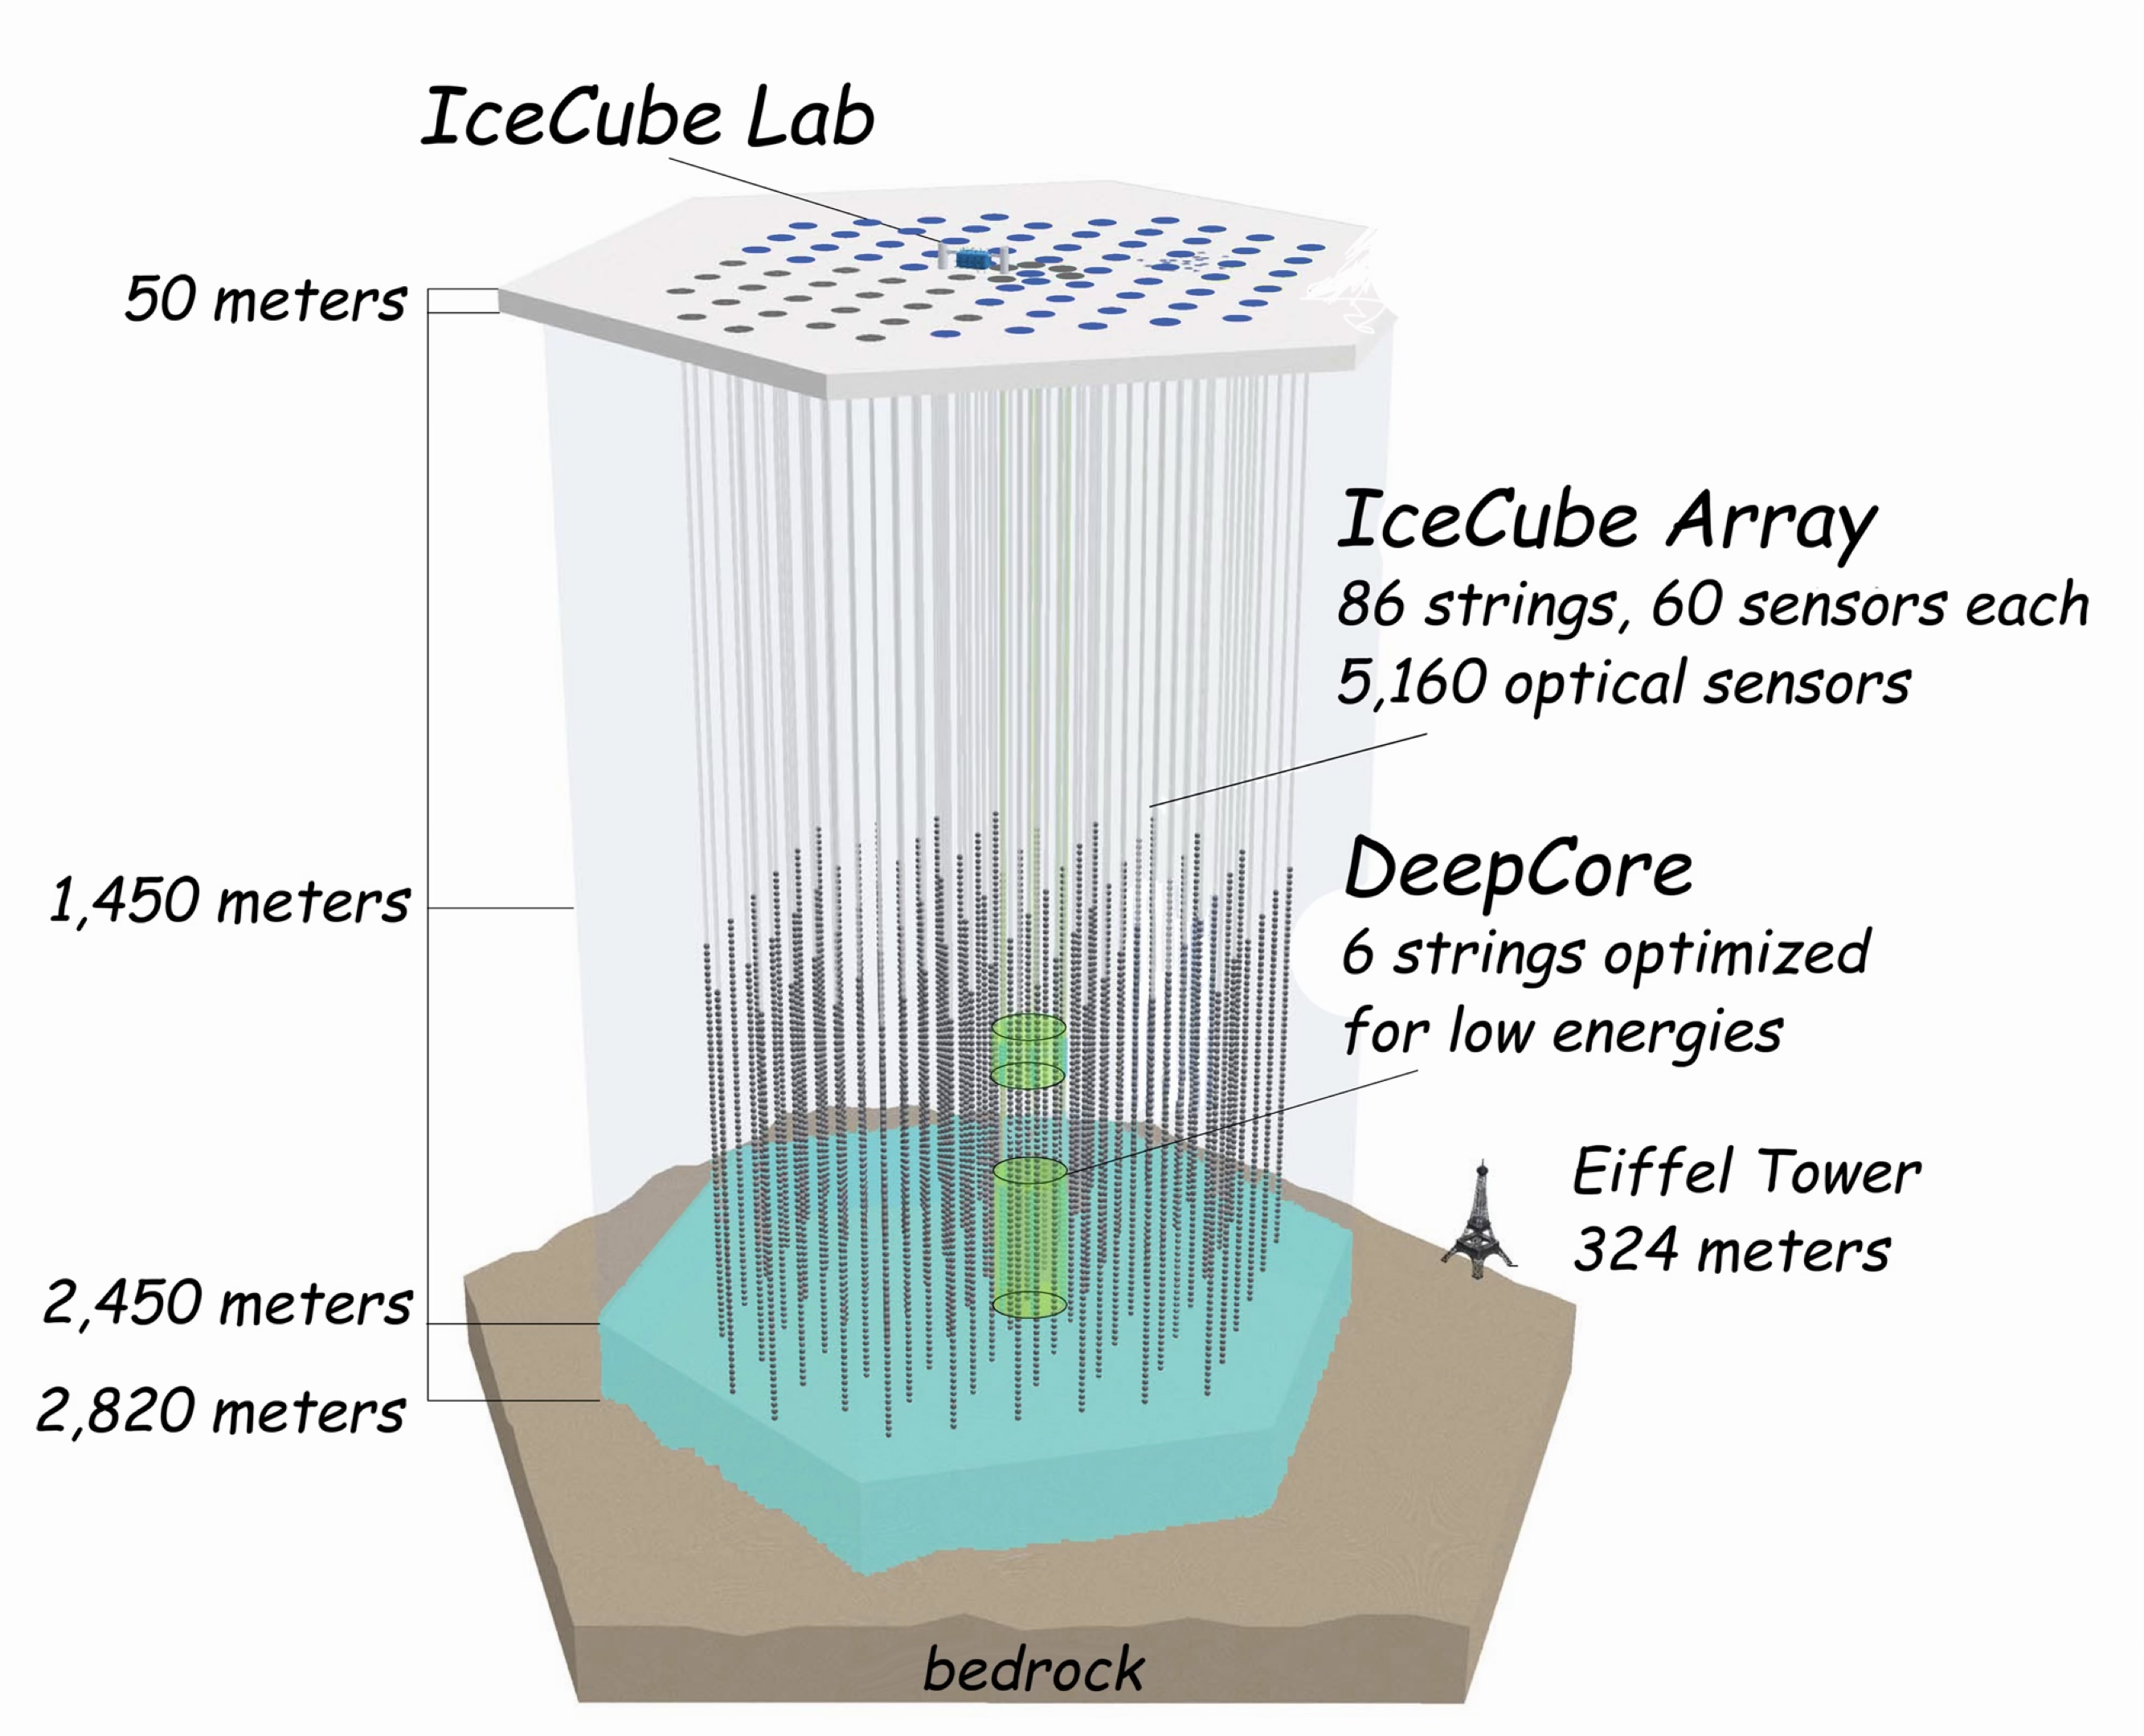
\includegraphics[width=\textwidth,height=0.70\textheight,keepaspectratio]{IceCubeInside.jpg}
 \column{0.5\textwidth}
      
   $\bullet$~El detector IceCube, bajo el hielo de la Antártida, es el aparato científico más grande construido por la humanidad. Es capaz de detectar neutrinos de energías extraordinarias.
   
   $\bullet$~La interacción de uno de esos neutrinos ilumina una superficie de sensores de IceCube equivalente a las partes viejas de Donostia y Bilbao \emph{juntas}.
  \end{columns}
\end{frame}



\begin{frame}{Neutrinos galácticos (y extragalácticos)}
  \begin{columns}
  \column{0.5\textwidth}
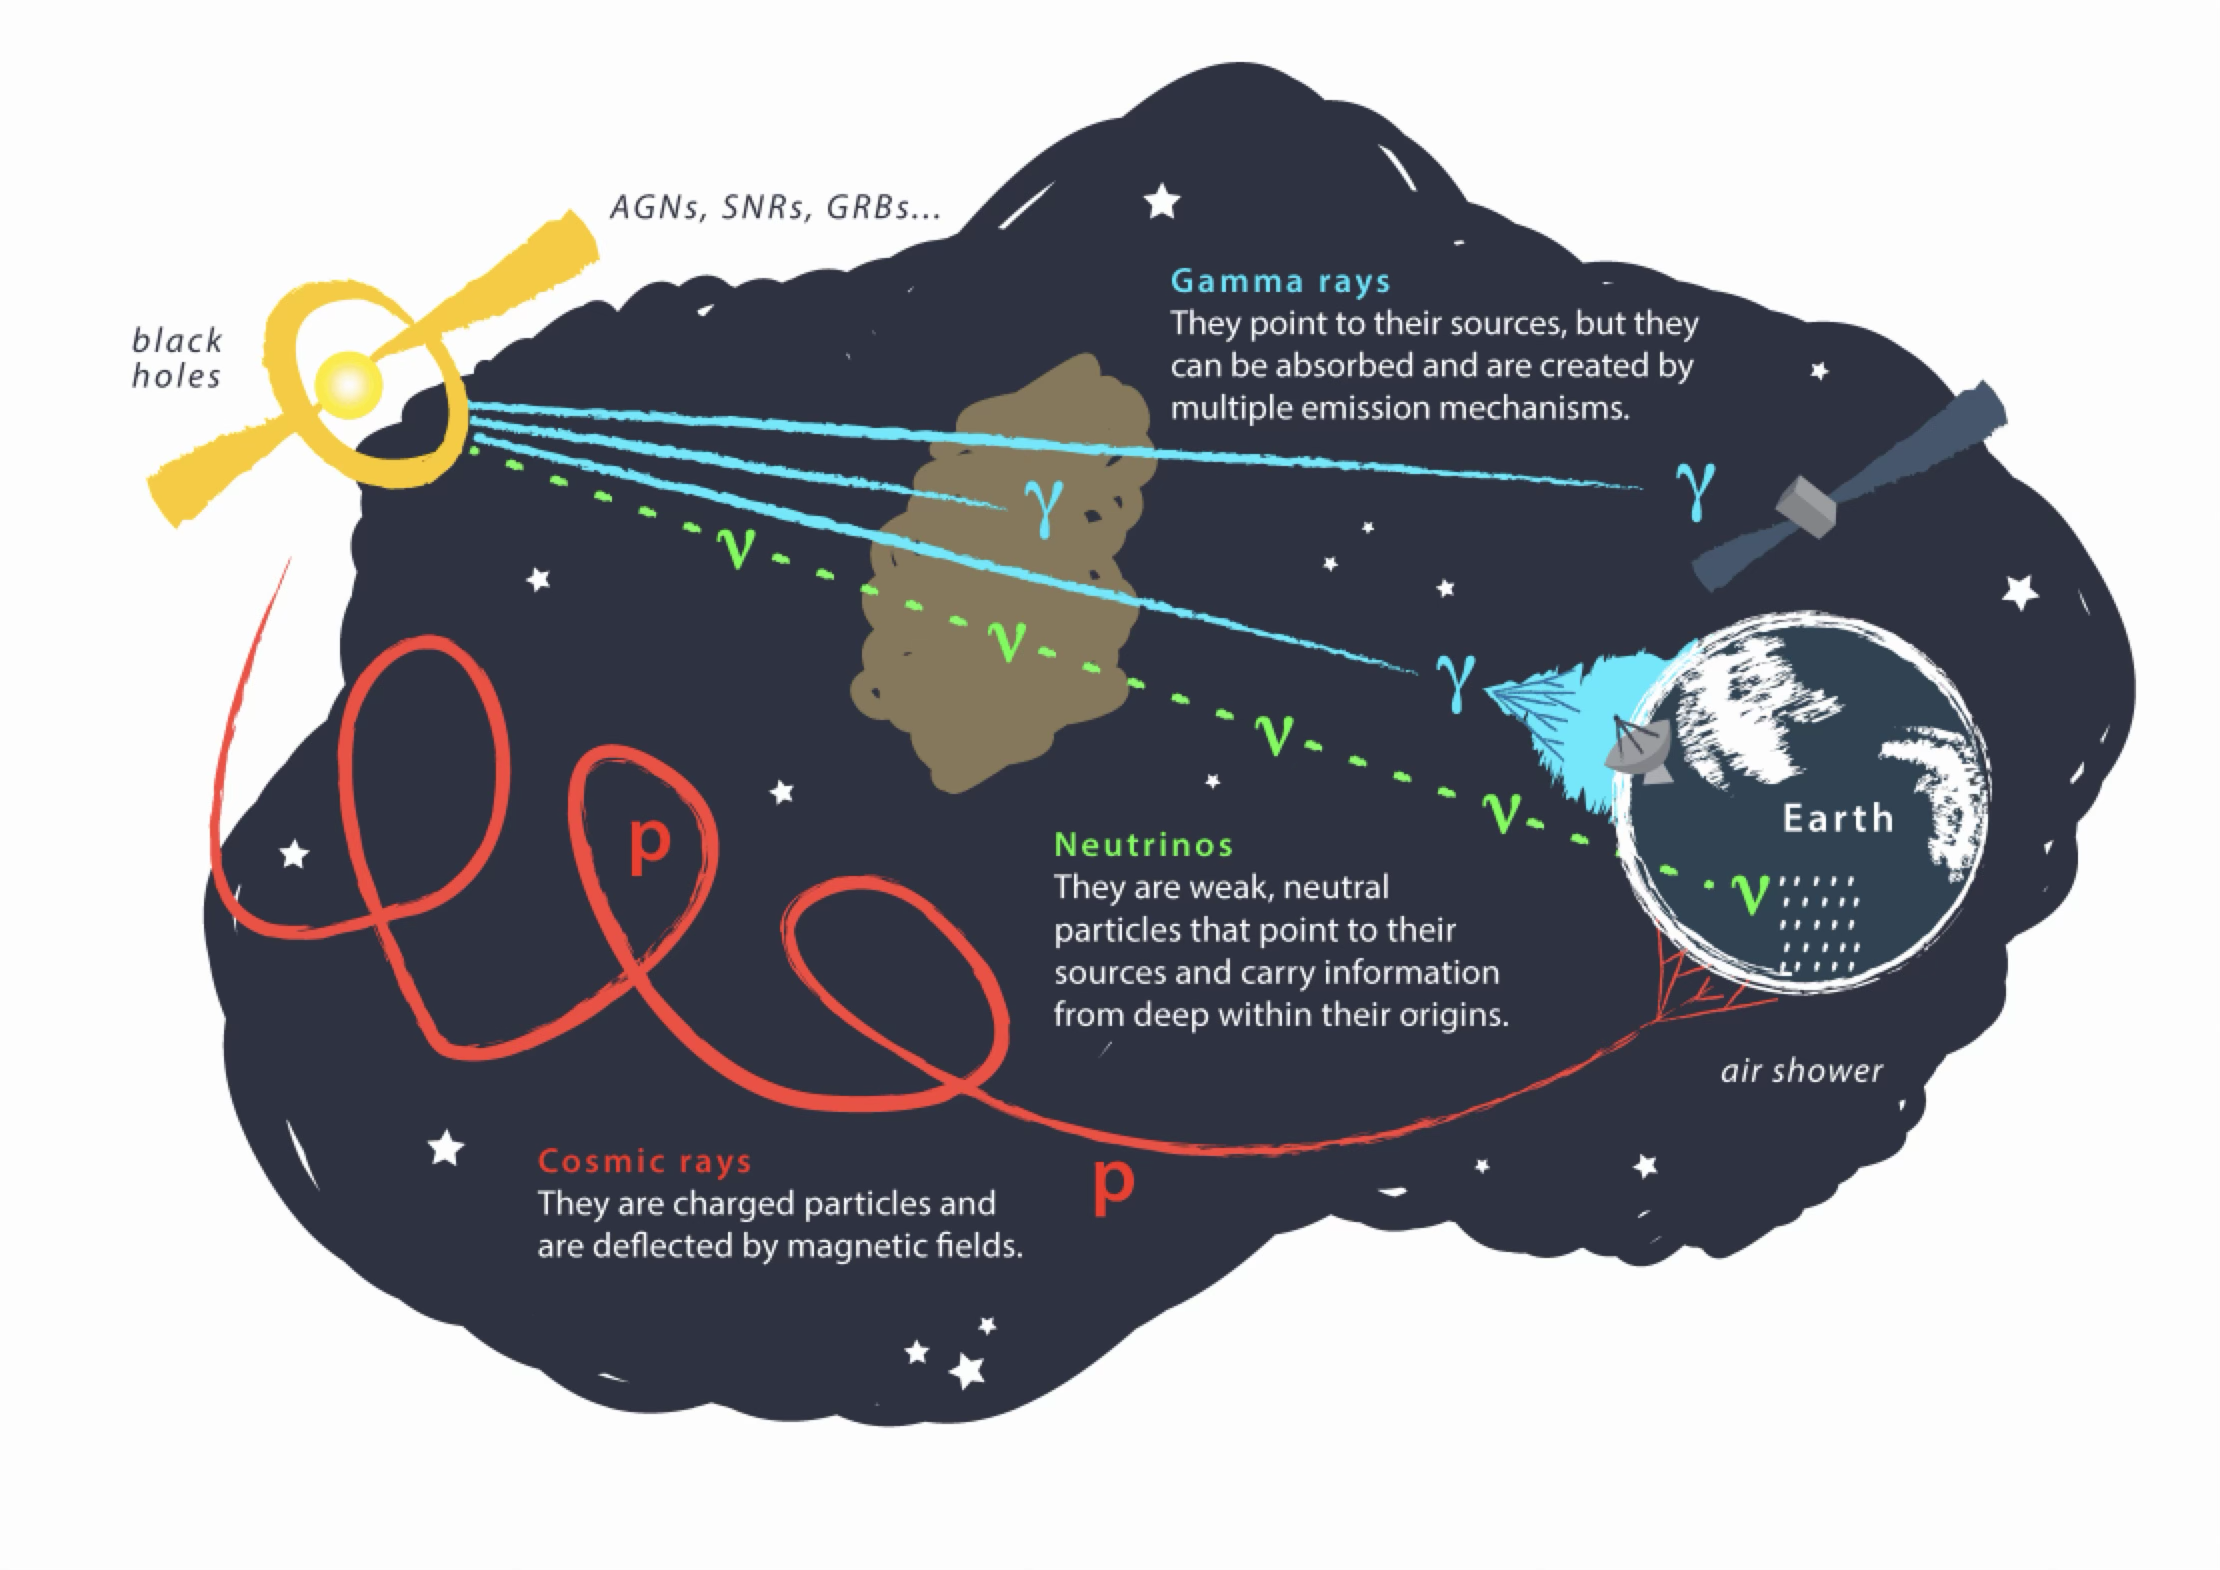
\includegraphics[width=\textwidth,height=0.70\textheight,keepaspectratio]{agn.png}
 \column{0.5\textwidth}
      
   $\bullet$~IceCube detecta neutrinos producidos en eventos extremadamente violentos en la galaxia (y fuera de ella), tales como <<aceleradores cósmicos>>.  
   
   $\bullet$~Eso nos permite entender el Universo mejor, utilizando la <<banda de radio de neutrinos>>.
  \end{columns}
\end{frame}


\begin{frame}{Sir Arthur, quizás tendrás que creer}
  \begin{columns}
  \column{0.5\textwidth}
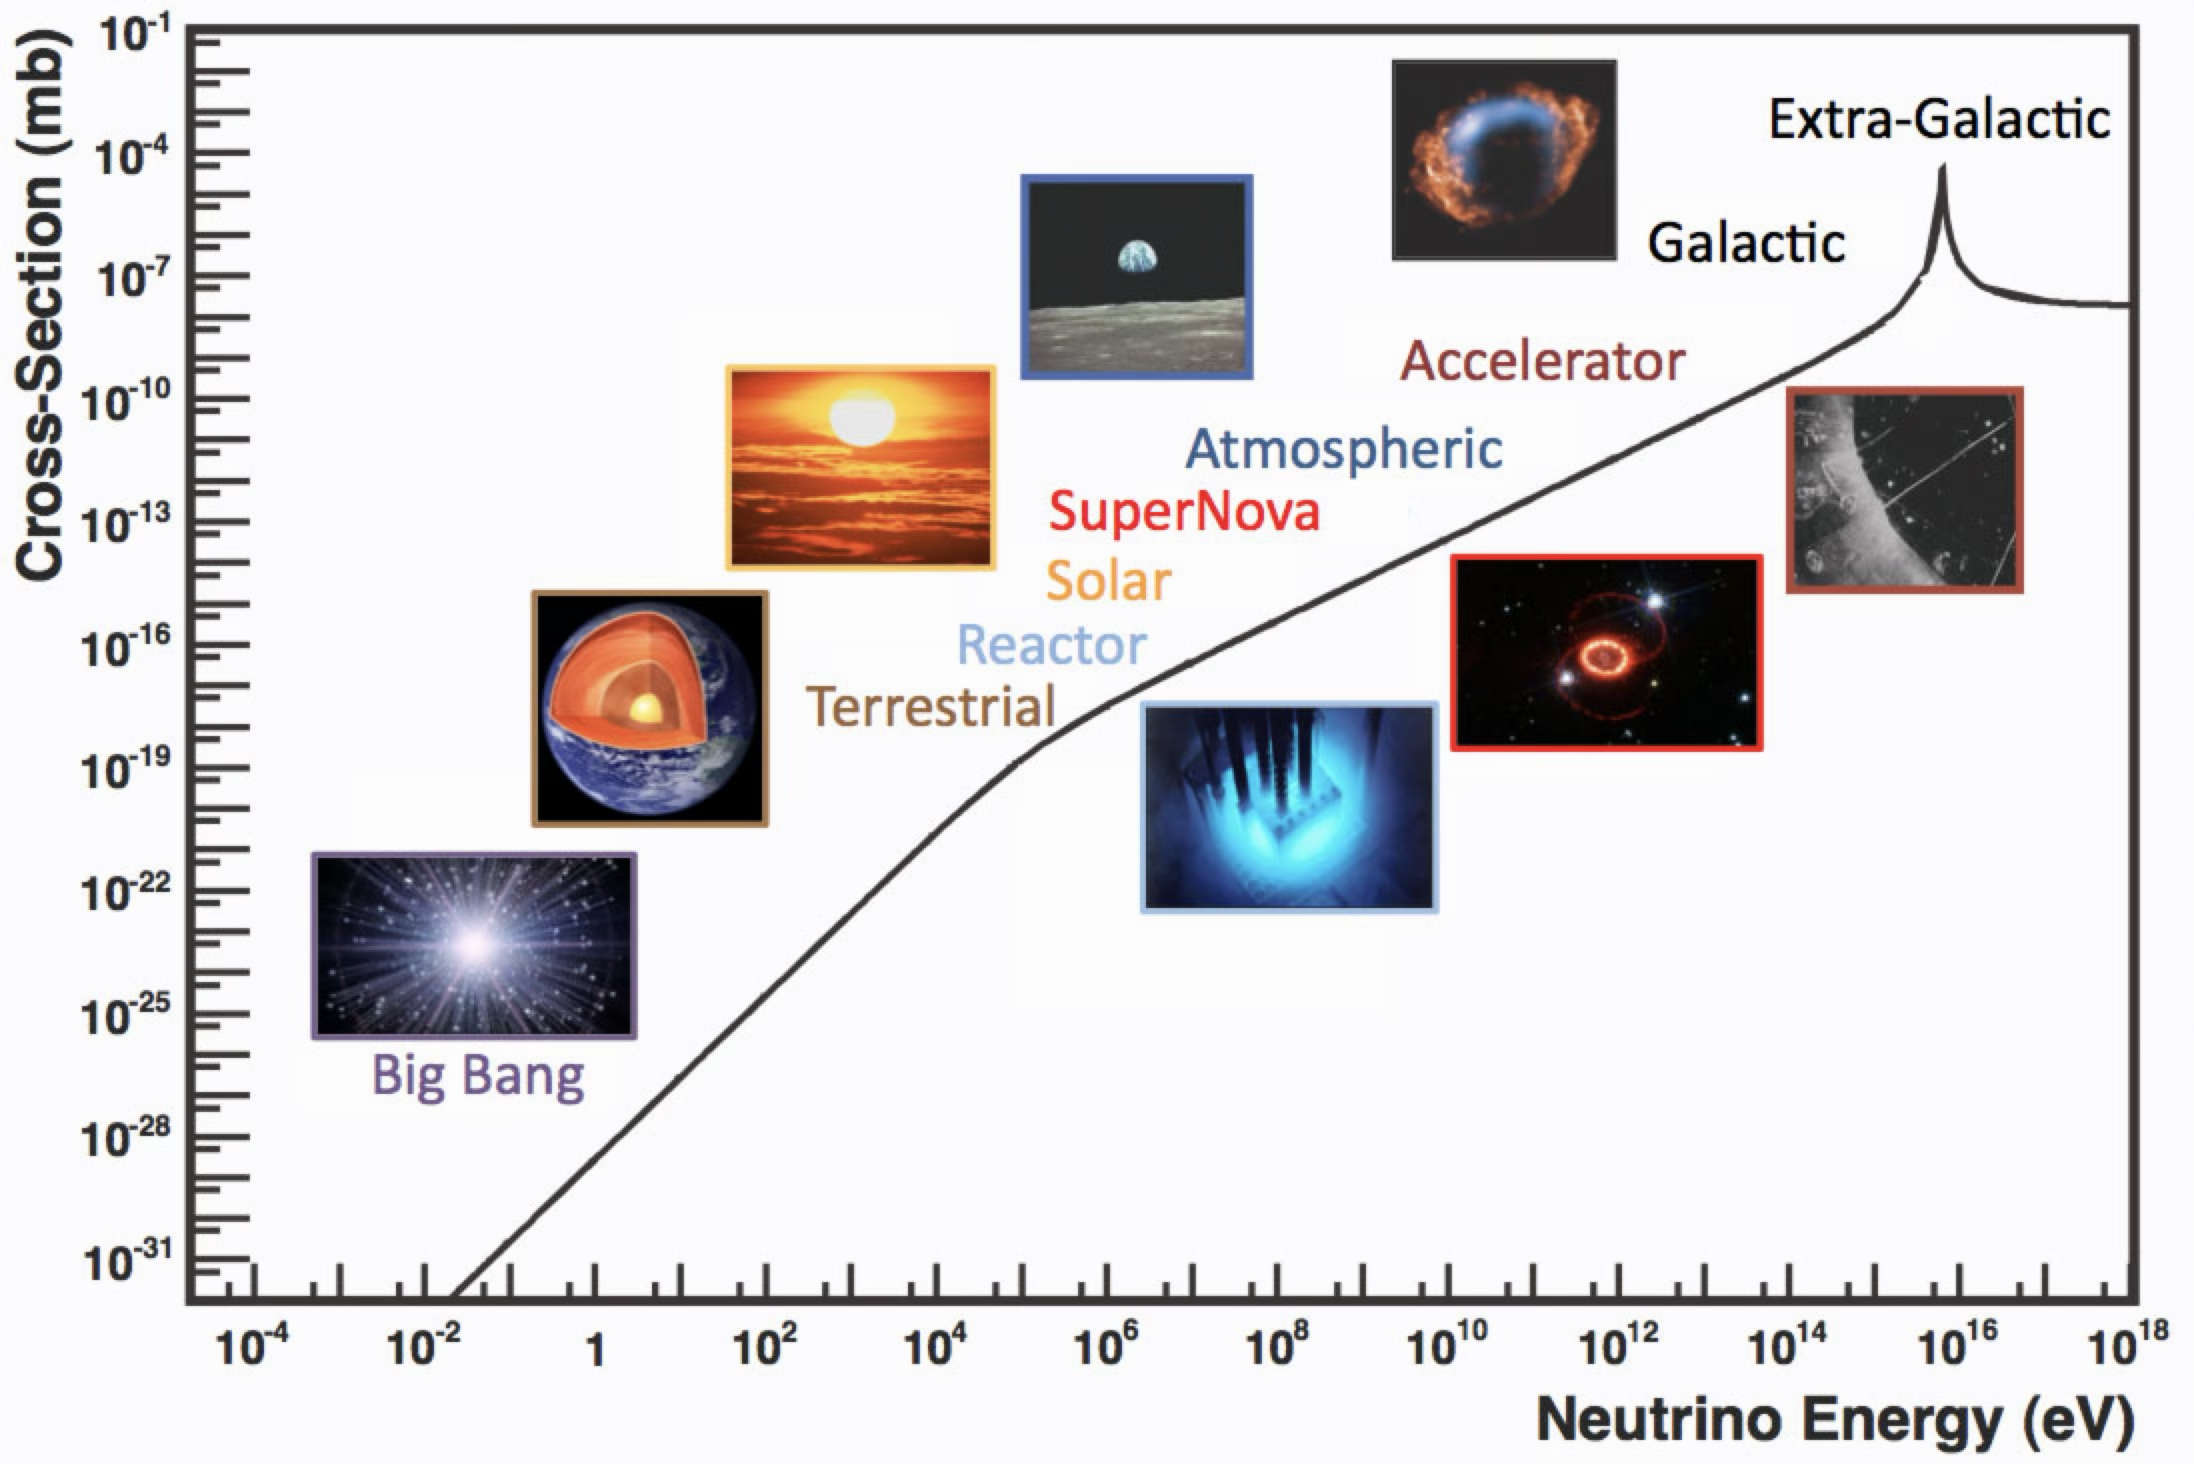
\includegraphics[width=\textwidth,height=0.70\textheight,keepaspectratio]{nusources.png}
 \column{0.5\textwidth}
      
   $\bullet$~En 2026 los físicos han tenido el ingenio de detectar neutrinos procedentes del Sol, de la atmósfera, del centro de la Tierra, de una supernova y neutrinos de alta energía producidos en aceleradores cósmicos.  
   
   $\bullet$~¿Qué opinas, sir Arthur?
  \end{columns}
\end{frame}



\begin{frame}{¿Sirven para algo los neutrinos?}
   \frase{¿Sirven para algo los unicornios?}
\end{frame}


% =====================================================================
% 2. UNICORNIO 2: EL POSITRÓN Y LA ANTIMATERIA
% =====================================================================
%\begin{frame}{Y dijo Dirac: Hágase el positrón}
%  \begin{columns}
%  \column{0.4\textwidth}
%    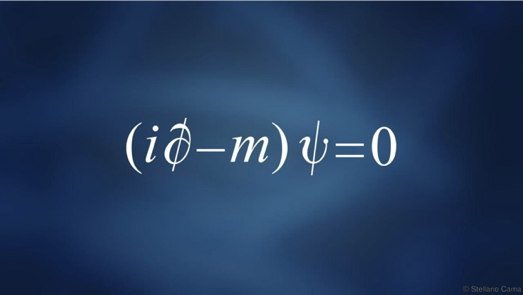
\includegraphics[width=\textwidth,height=0.30\textheight,keepaspectratio]{dirac-eq.png}
%    
%    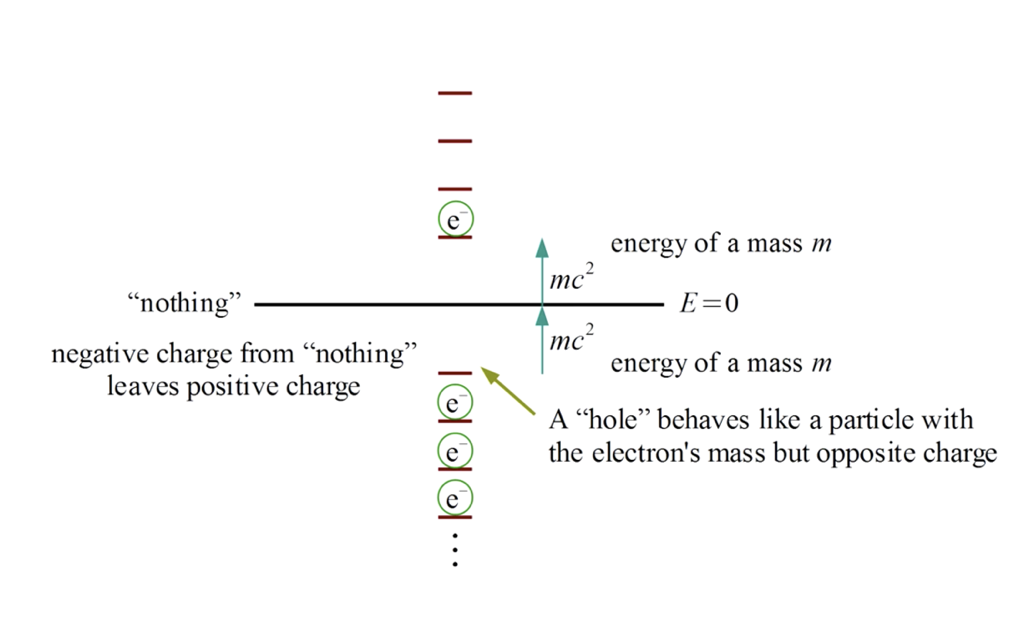
\includegraphics[width=\textwidth,height=0.70\textheight,keepaspectratio]{negativeSea.png}
%  \column{0.58\textwidth}
%%    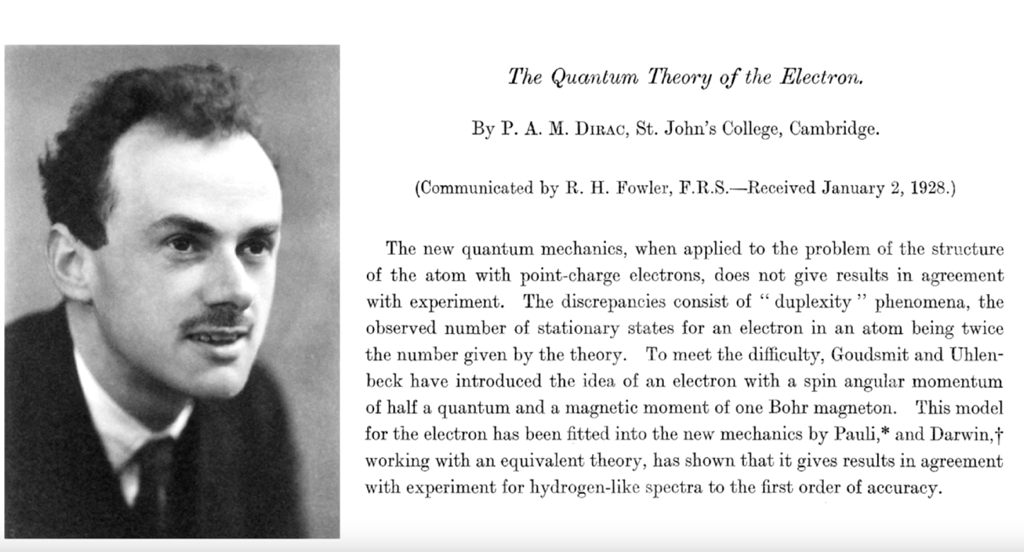
\includegraphics[width=\textwidth]{dirac-eq-paper.png}\\[1ex]
%$\bullet$~En 1928, P.A.M. Dirac dio con una ecuación que describía el comportamiento de los electrones relativistas, conjuntando la mecánica cuántica y la relatividad (por la época ambas teorías eran nuevas y revolucionarias).   %    relatividad.
%
%$\bullet$~La ecuación predice tantas soluciones de energía negativa como positiva. Dirac reinterpreta las soluciones de energía negativa como electrones de carga positiva, inventando otro unicornio. La antimateria. 
%  \end{columns}
%\end{frame}

%\begin{frame}{Soluciones de más}
%  \begin{columns}
%  \column{0.55\textwidth}
%    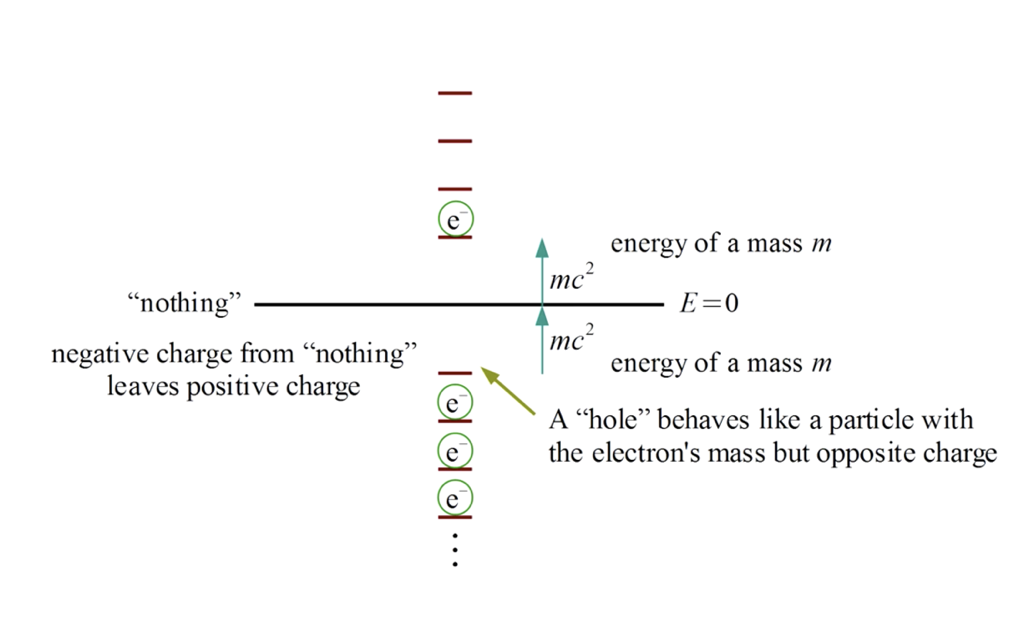
\includegraphics[width=\textwidth]{negativeSea.png}
%  \column{0.45\textwidth}
%    La ecuación tiene tantas soluciones de energía negativa como positiva.\\[1ex]
%    Dirac no las tira. Imagina un mar infinito de electrones invisibles, y
%    ``agujeros'' en ese mar.\\[1ex]
%    Primero intenta que los agujeros sean protones (1929). No funciona.
%  \end{columns}
%\end{frame}
%
%\begin{frame}{Heisenberg contra Dirac}
%  \begin{columns}
%  \column{0.55\textwidth}
%    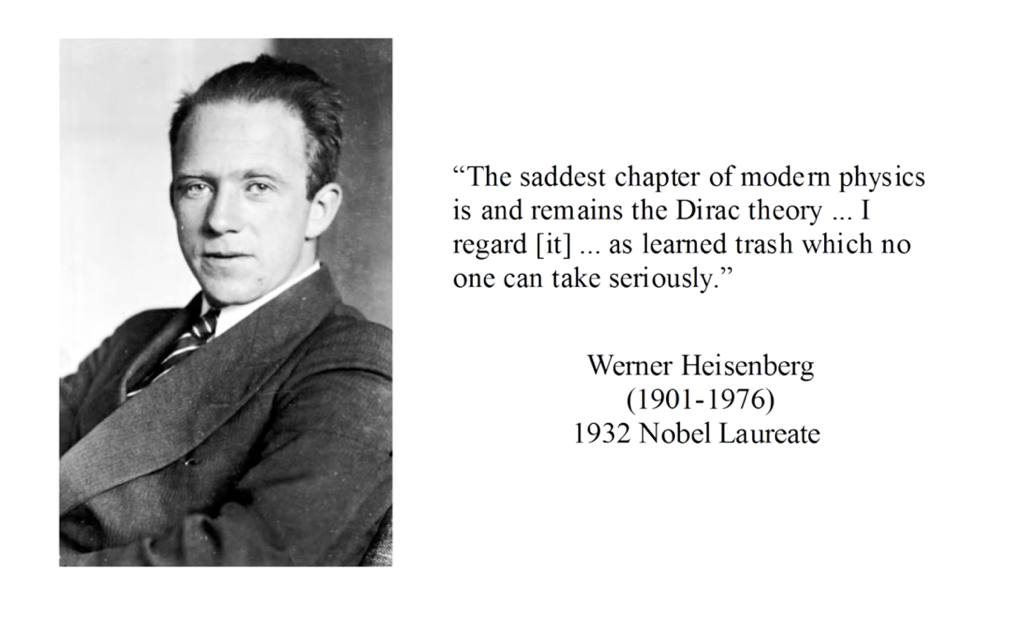
\includegraphics[width=\textwidth]{HeisembergOpinionDirac.png}
%  \column{0.45\textwidth}
%    \begin{cita}
%    El capítulo más triste de la física moderna es y sigue siendo la teoría
%    de Dirac\dots\ La considero basura erudita que nadie puede tomarse en
%    serio.
%    \end{cita}
%    \hfill Werner Heisenberg
%  \end{columns}
%\end{frame}
%
%\begin{frame}{1931: el anti-electrón}
%  \begin{columns}
%  \column{0.6\textwidth}
%    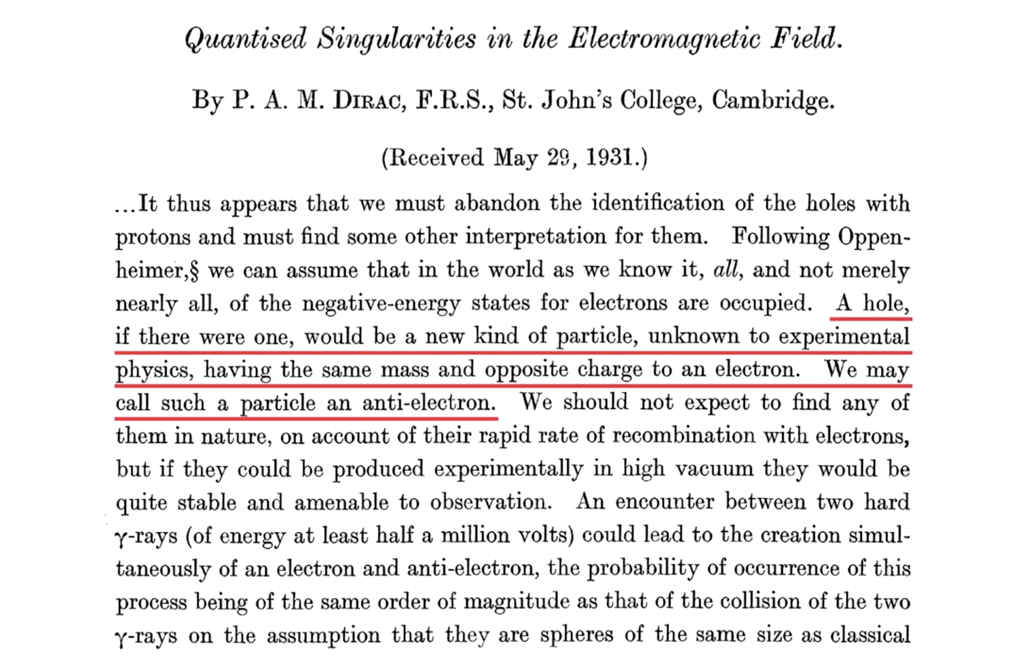
\includegraphics[width=\textwidth]{diracPositrons.png}
%  \column{0.4\textwidth}
%    \begin{cita}
%    Un agujero, si existiera, sería una nueva clase de partícula, desconocida
%    para la física experimental, con la misma masa y carga opuesta a la del
%    electrón. Podemos llamarla anti-electrón.
%    \end{cita}
%    \hfill P.A.M. Dirac
%  \end{columns}
%\end{frame}

\begin{frame}{Antimateria}
 % \begin{columns}
  %\column{0.45\textwidth}
  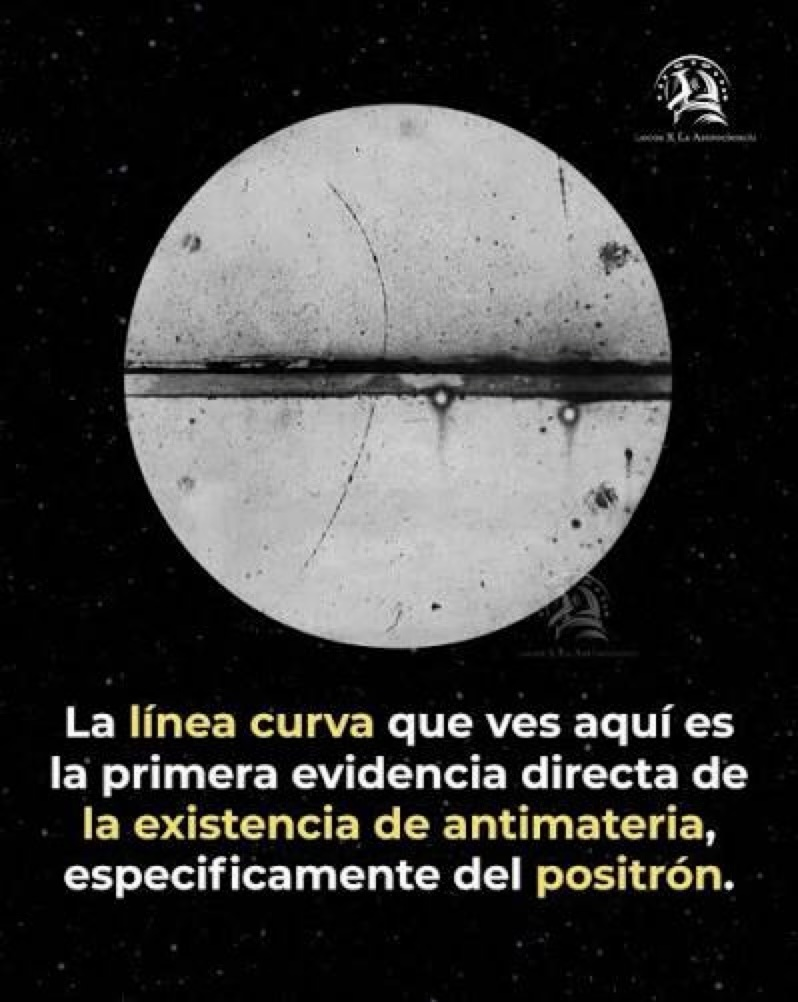
\includegraphics[width=\textwidth,height=0.50\textheight,keepaspectratio]{positronBubble.jpg}    
    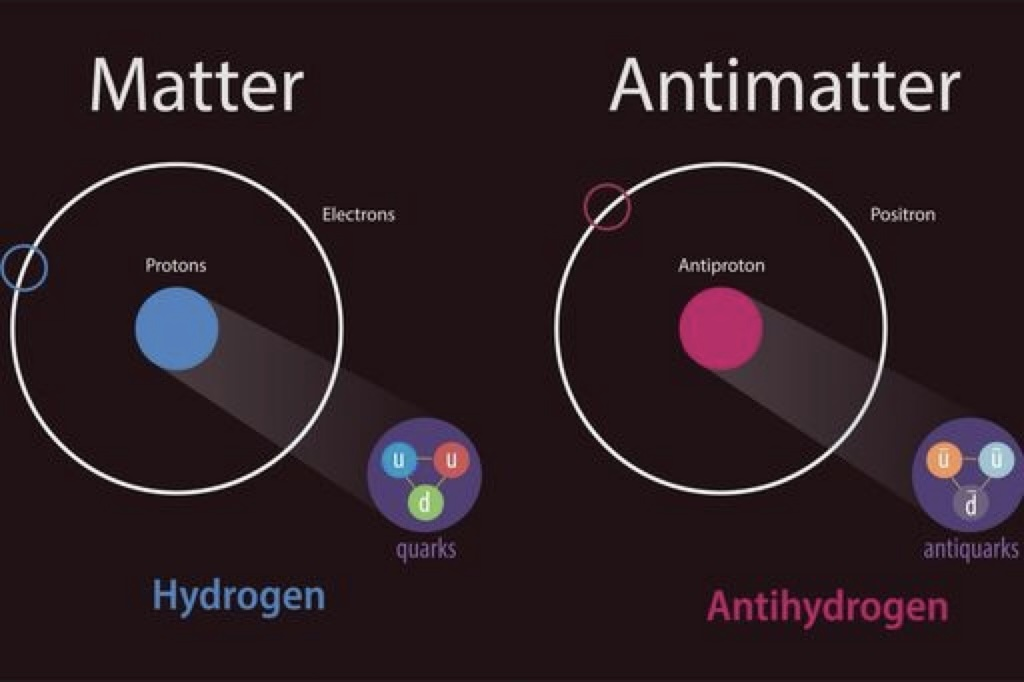
\includegraphics[width=\textwidth,height=0.50\textheight,keepaspectratio]{antimatter.jpg}
    
      {\footnotesize\color{gray}Detección del positrón. Anderson, 1932.}

    
%  \column{0.55\textwidth}
   $\bullet$~Las partículas de antimateria son idénticas a las de materia, con todas las cargas invertidas. 
   
      
%  \end{columns}
\end{frame}


\begin{frame}{La materia y la antimateria se aniquilan}
 \begin{columns}
  \column{0.50\textwidth}
  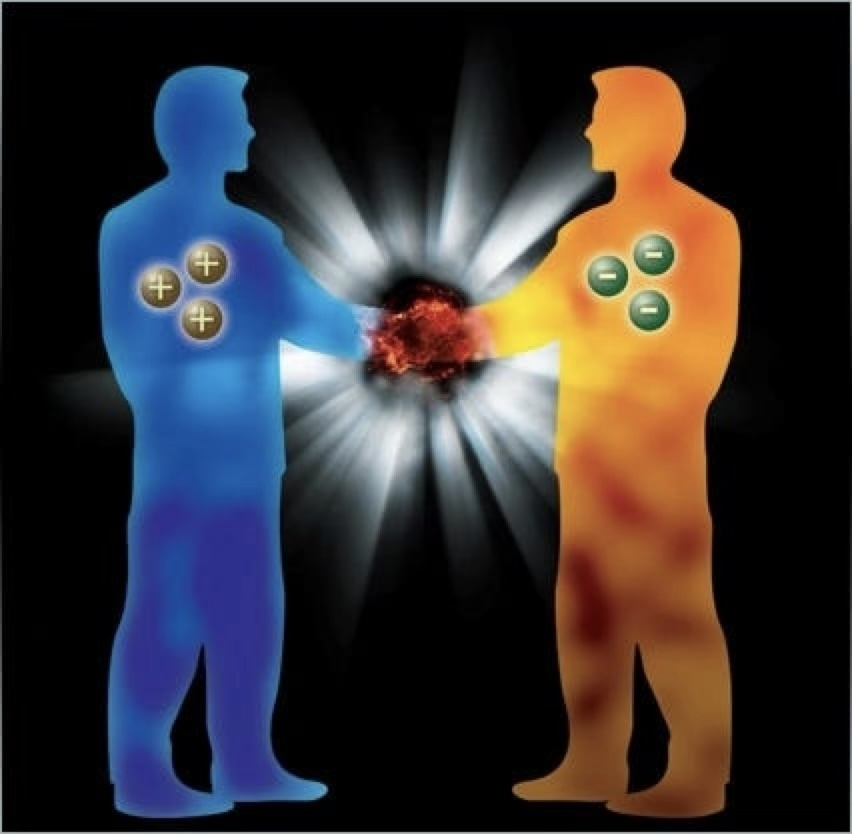
\includegraphics[width=\textwidth,height=0.80\textheight,keepaspectratio]{shakeMatterAntimatter.jpg}    
    
    
 \column{0.50\textwidth}
   $\bullet$~Materia y antimateria se aniquilan, produciendo energía en forma de rayos gamma. 
   
   $\bullet$~Si existieran galaxias de antimateria, algunas de ellas colisionarían con galaxias de materia y el resultado sería una emisión de energía extraordinaria, que nuestros aparatos no han detectado. Por otra parte, en la Tierra y en nuestro sistema solar, nuestros aparatos miden que apenas hay antimateria. 
      
 \end{columns}
\end{frame}

%\begin{frame}{Anderson, 1932}
%  \begin{columns}
%  \column{0.6\textwidth}
%    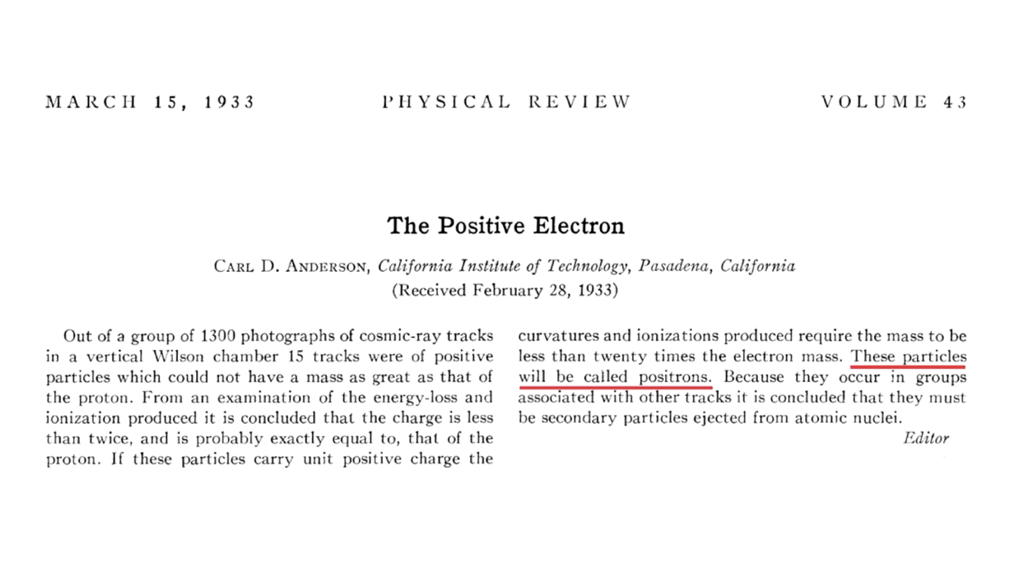
\includegraphics[width=\textwidth]{AndersonPaper.png}
%  \column{0.4\textwidth}
%    \pendiente[0.35\textheight]{Foto original de la traza del positrón en la cámara de niebla de Anderson.}
%    Lo encuentra en los rayos cósmicos y lo bautiza \textbf{positrón}.\\[1ex]
%    Dirac esperó un año. Pauli esperaría 26.
%  \end{columns}
%\end{frame}

\begin{frame}{¿Por qué existe el Universo?}
  \begin{columns}
  \column{0.5\textwidth}
 
    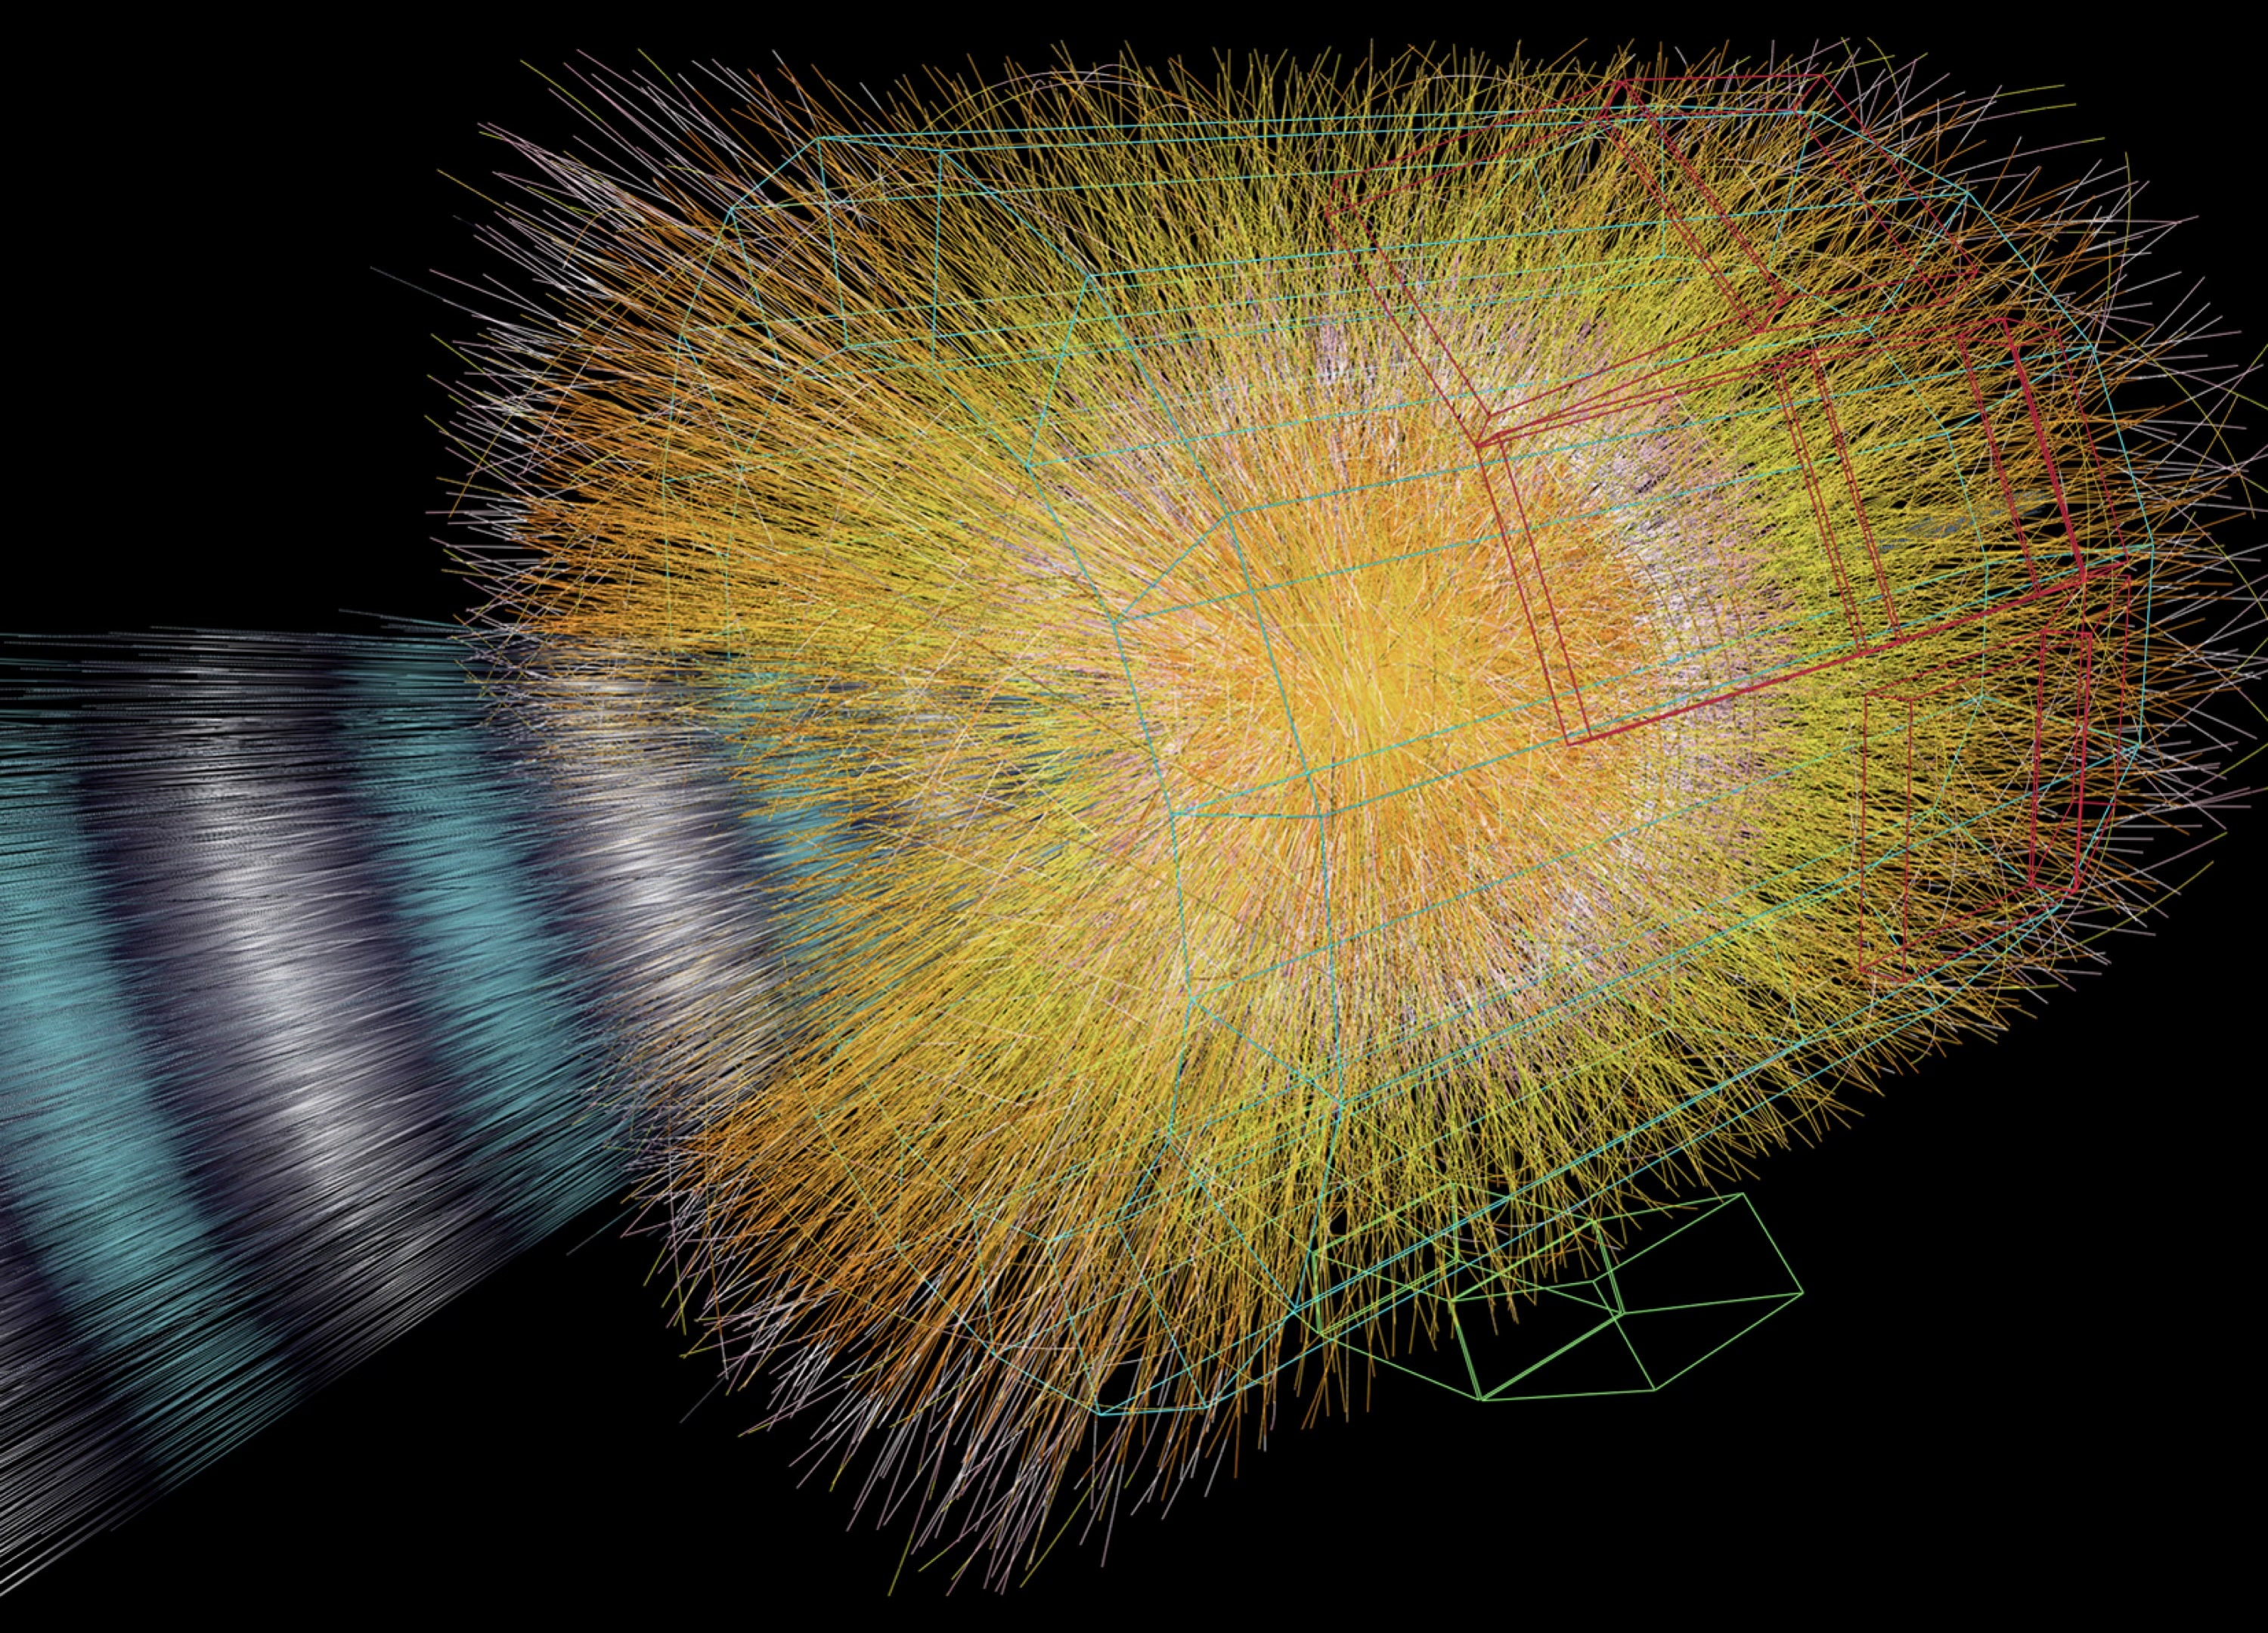
\includegraphics[width=\textwidth,height=0.70\textheight,keepaspectratio]{lhcCollision.jpg}
     {\footnotesize\color{gray} Un <<mini Big Bang>> producido en el LHC del CERN}
  \column{0.5\textwidth}
    
    $\bullet$~Todos los experimentos indican que la materia y la antimateria se producen siempre de manera simétrica, es decir, por pares partícula-antipartícula. 
    
    $\bullet$~En el Big Bang debería haberse producido la misma cantidad de materia que de antimateria. 
    
    $\bullet$~Pero la materia y la antimateria se aniquilan al encontrarse. Justo después del Big Bang, la densidad de partículas y antipartículas era tan grande que la aniquilación era inevitable y por tanto el Universo debería haber <<explotado en luz>> inmediatamente después de formarse.
    
  \end{columns}
\end{frame}

%\begin{frame}{El Big Bang debió crear tanta materia como antimateria}
%  \begin{columns}
%  \column{0.55\textwidth}
%    
\includegraphics[width=\textwidth]{MissingUniverse.png}
%  \column{0.45\textwidth}
%    Un Universo simétrico se aniquila a sí mismo.\\[1ex]
%    Solo quedaría luz. Ni galaxias, ni estrellas, ni nosotros.
%  \end{columns}
%\end{frame}
%
%\begin{frame}
%  \frase{Y sin embargo hay Universo.\\[1ex] ¿Dónde fue la antimateria?}
%\end{frame}
%
%% =====================================================================
%% 3. ¿PARA QUÉ SIRVEN LOS NEUTRINOS?
%% =====================================================================
%\begin{frame}{Reines y Cowan, 1956}
%  \begin{columns}
%  \column{0.5\textwidth}
%    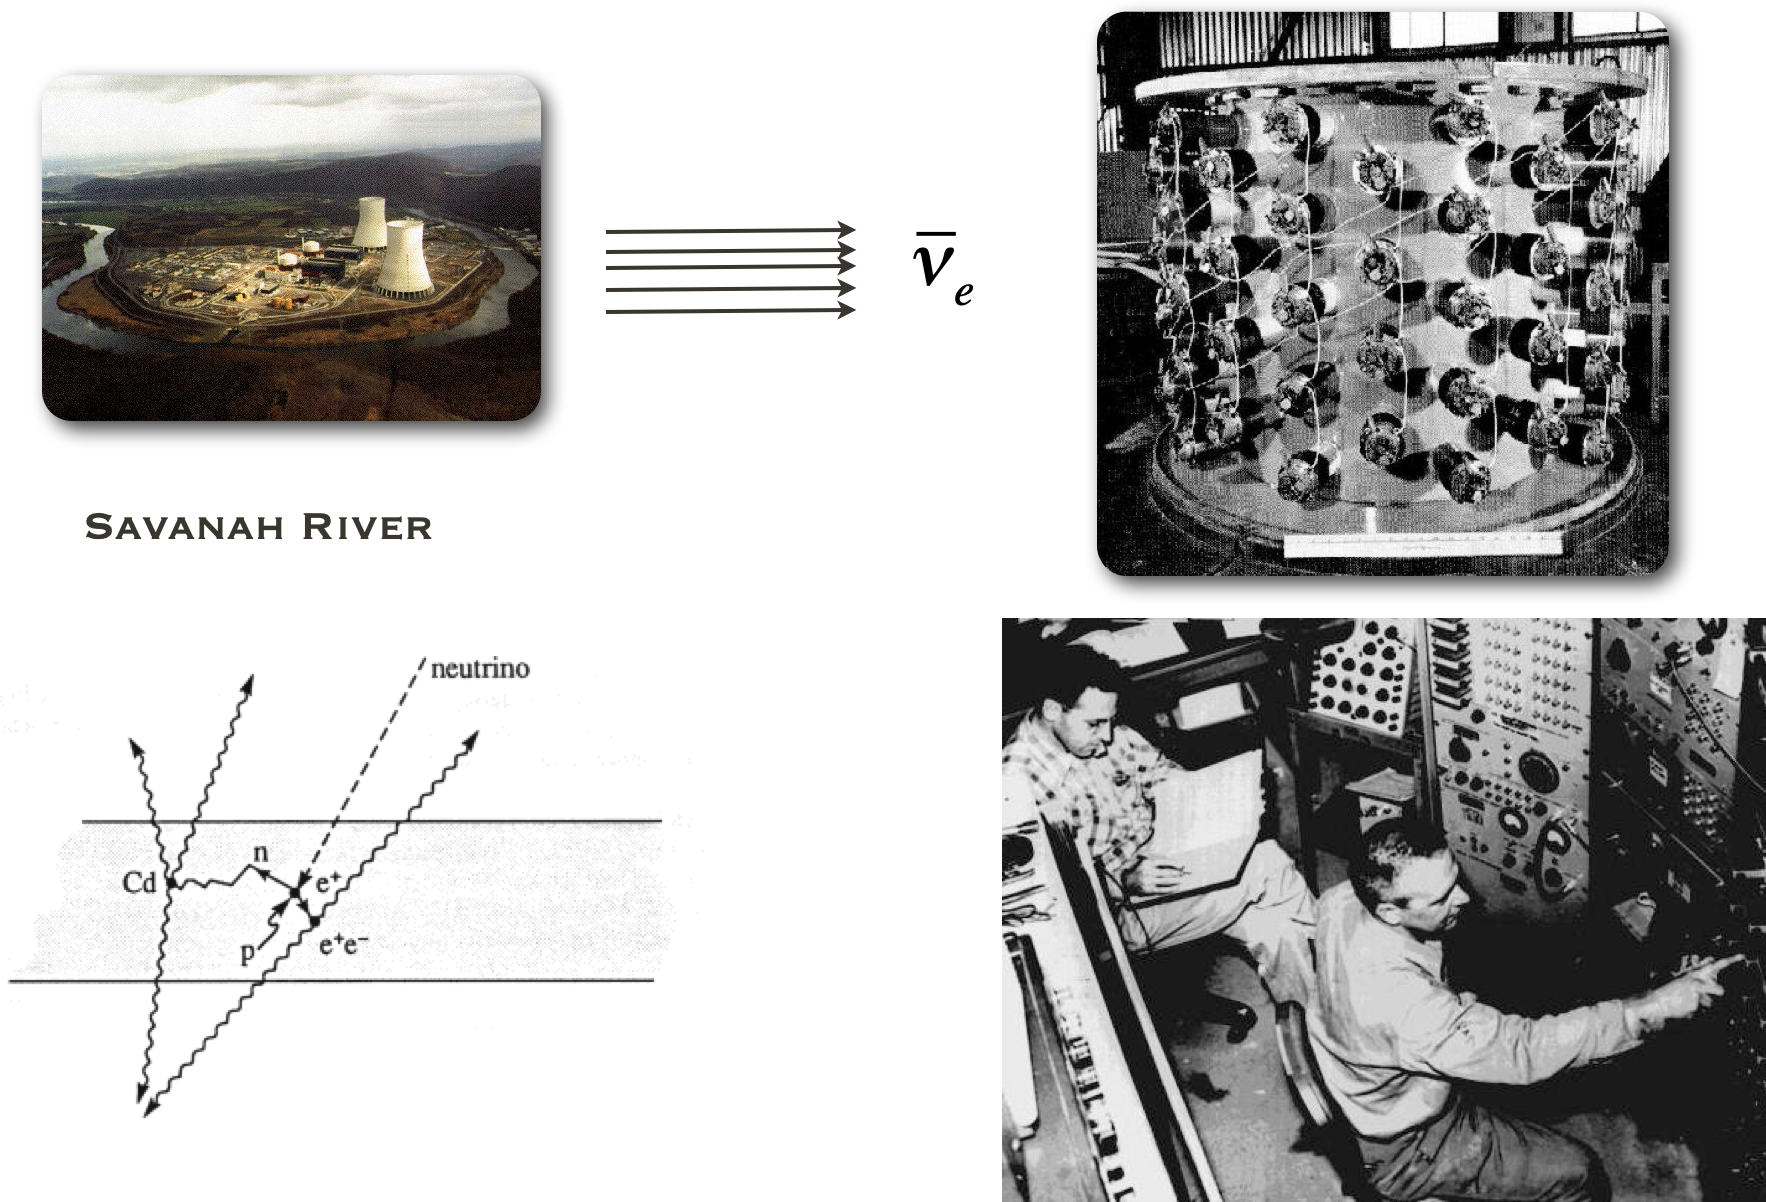
\includegraphics[width=\textwidth]{reinesCowan.png}
%  \column{0.5\textwidth}
%    Un reactor nuclear emite \textbf{cien trillones} de antineutrinos por
%    segundo.\\[1ex]
%    Con tantos, alguno tiene que chocar.\\[1ex]
%    Detector: un tanque de agua junto al reactor de Savannah River.
%  \end{columns}
%\end{frame}
%
%\begin{frame}{Los dos unicornios juntos}
%  \begin{columns}
%  \column{0.55\textwidth}
%    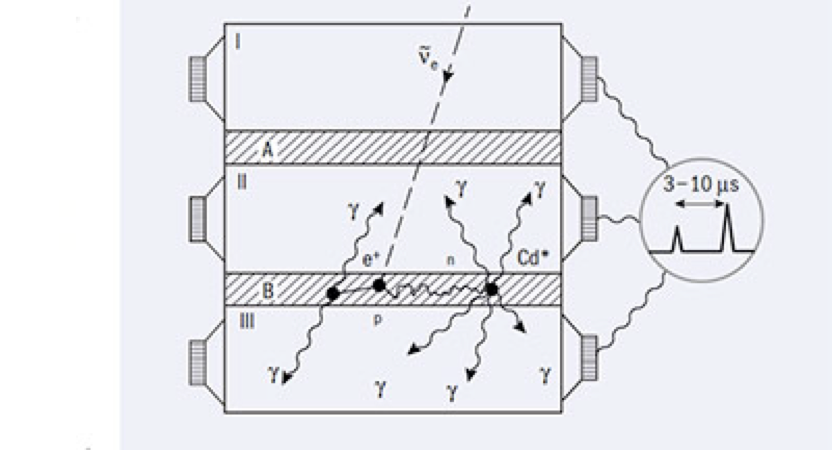
\includegraphics[width=\textwidth]{doubleCoincidence.png}
%  \column{0.45\textwidth}
%    El antineutrino choca con un protón y produce \textbf{un positrón} y un
%    neutrón.\\[1ex]
%    El positrón se aniquila: dos fotones.\\
%    Microsegundos después, el neutrón es capturado: más fotones.\\[1ex]
%    La \textbf{coincidencia retardada}: una firma inconfundible.\\[1ex]
%    Arthur, tendrás que creer.
%  \end{columns}
%\end{frame}

\begin{frame}{¿Sirven para algo los neutrinos?}
   \frase{Sirven (posiblemente) para crear universos}
\end{frame}

\begin{frame}{El neutrino de Majorana}
  \begin{columns}
  \column{0.4\textwidth}
    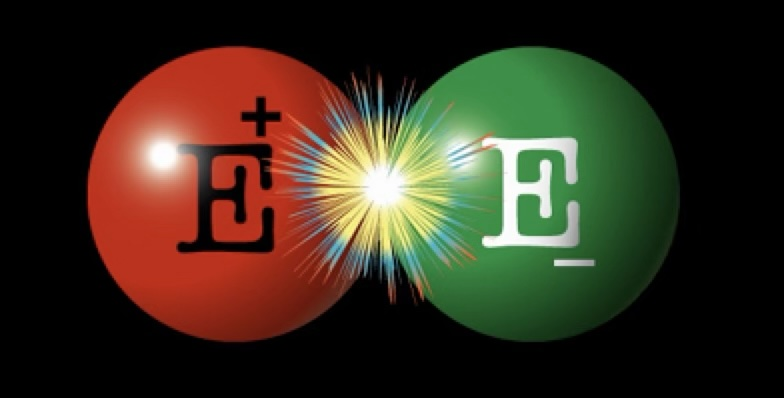
\includegraphics[width=\textwidth,height=0.25\textheight,keepaspectratio]{eplueminus.jpg}
    
     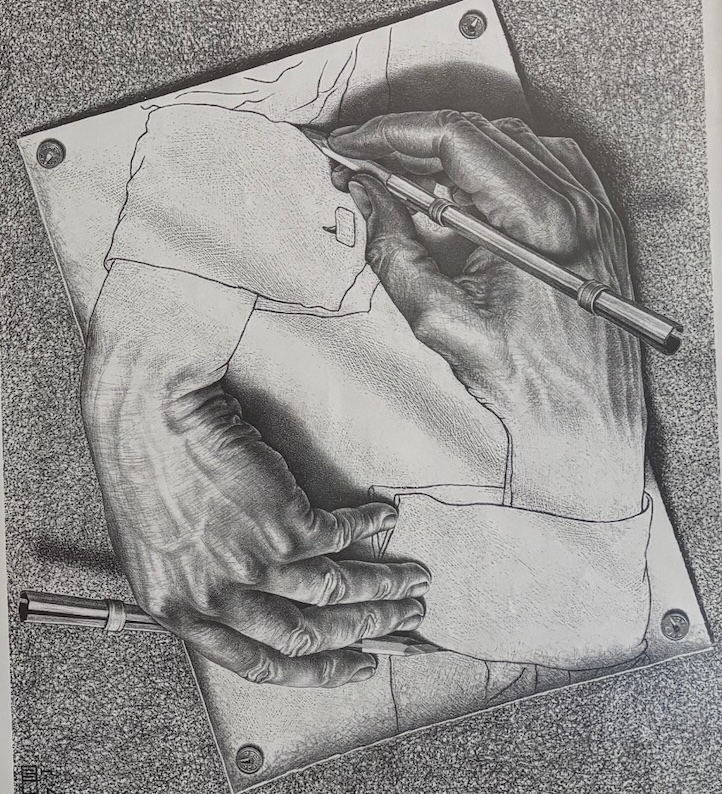
\includegraphics[width=\textwidth,height=0.55\textheight,keepaspectratio]{echerHands.jpg}
    
   
  \column{0.6\textwidth}
     
    $\bullet$~A diferencia de los electrones (y el resto de las partículas elementales), el neutrino no tiene carga eléctrica y por tanto la conjugación de carga al pasar de materia a antimateria ($e^- \rightarrow e^+$) no le afecta ($\nu \rightarrow \nu$). De ahí que sea posible, matemáticamente, describir al neutrino como su propia antipartícula $\nu = \bar{\nu}$ (Ettore Majorana, 1937). 
    
  \end{columns}
\end{frame}


\begin{frame}{Un agente doble}

\begin{columns}
\column{0.5\textwidth}

\includegraphics[width=\textwidth,height=0.30\textheight,keepaspectratio]{sumo_electron.png}
     
\includegraphics[width=\textwidth,height=0.30\textheight,keepaspectratio]{sumo_positron.png}
    
$\bullet$~Como $N$ es una partícula de materia, puede desintegrarse a un electrón ($e^-$), pero al ser también antimateria puede desintegrarse a un positrón ($e^+$). 


\column{0.45\textwidth}

$\bullet$~Imaginemos que en el Universo primitivo (justo después del Big Bang), además de $e^+$ y $e^-$ (materia y antimateria), se producen neutrinos pesados $N$ (antepasados de los actuales neutrinos), que son <<agentes dobles>>, por tanto, materia y antimateria a la vez. 


$\bullet$~Todos los agentes dobles favorecen, al final, a un bando más que a otro. Si $N$ favorecía ligeramente a la materia en sus desintegraciones, habría introducido una ligera asimetría. 
    
\end{columns}

\end{frame}

\begin{frame}{Nuestro Universo son los restos de un naufragio}
  \begin{columns}
  \column{0.4\textwidth}
    
\includegraphics[width=\textwidth]{MissingUniverse.png}
  \column{0.6\textwidth}
    
    $\bullet$~En el Universo temprano, la materia y antimateria originales (creadas en proporciones 50/50) se aniquilan entre sí. Solo sobrevive el pequeño exceso de materia introducido por $N$.
    
    $\bullet$~Esto explica por qué en nuestro Universo no hay (casi) antimateria. 
  \end{columns}
\end{frame}

\begin{frame}{La fórmula del Universo}

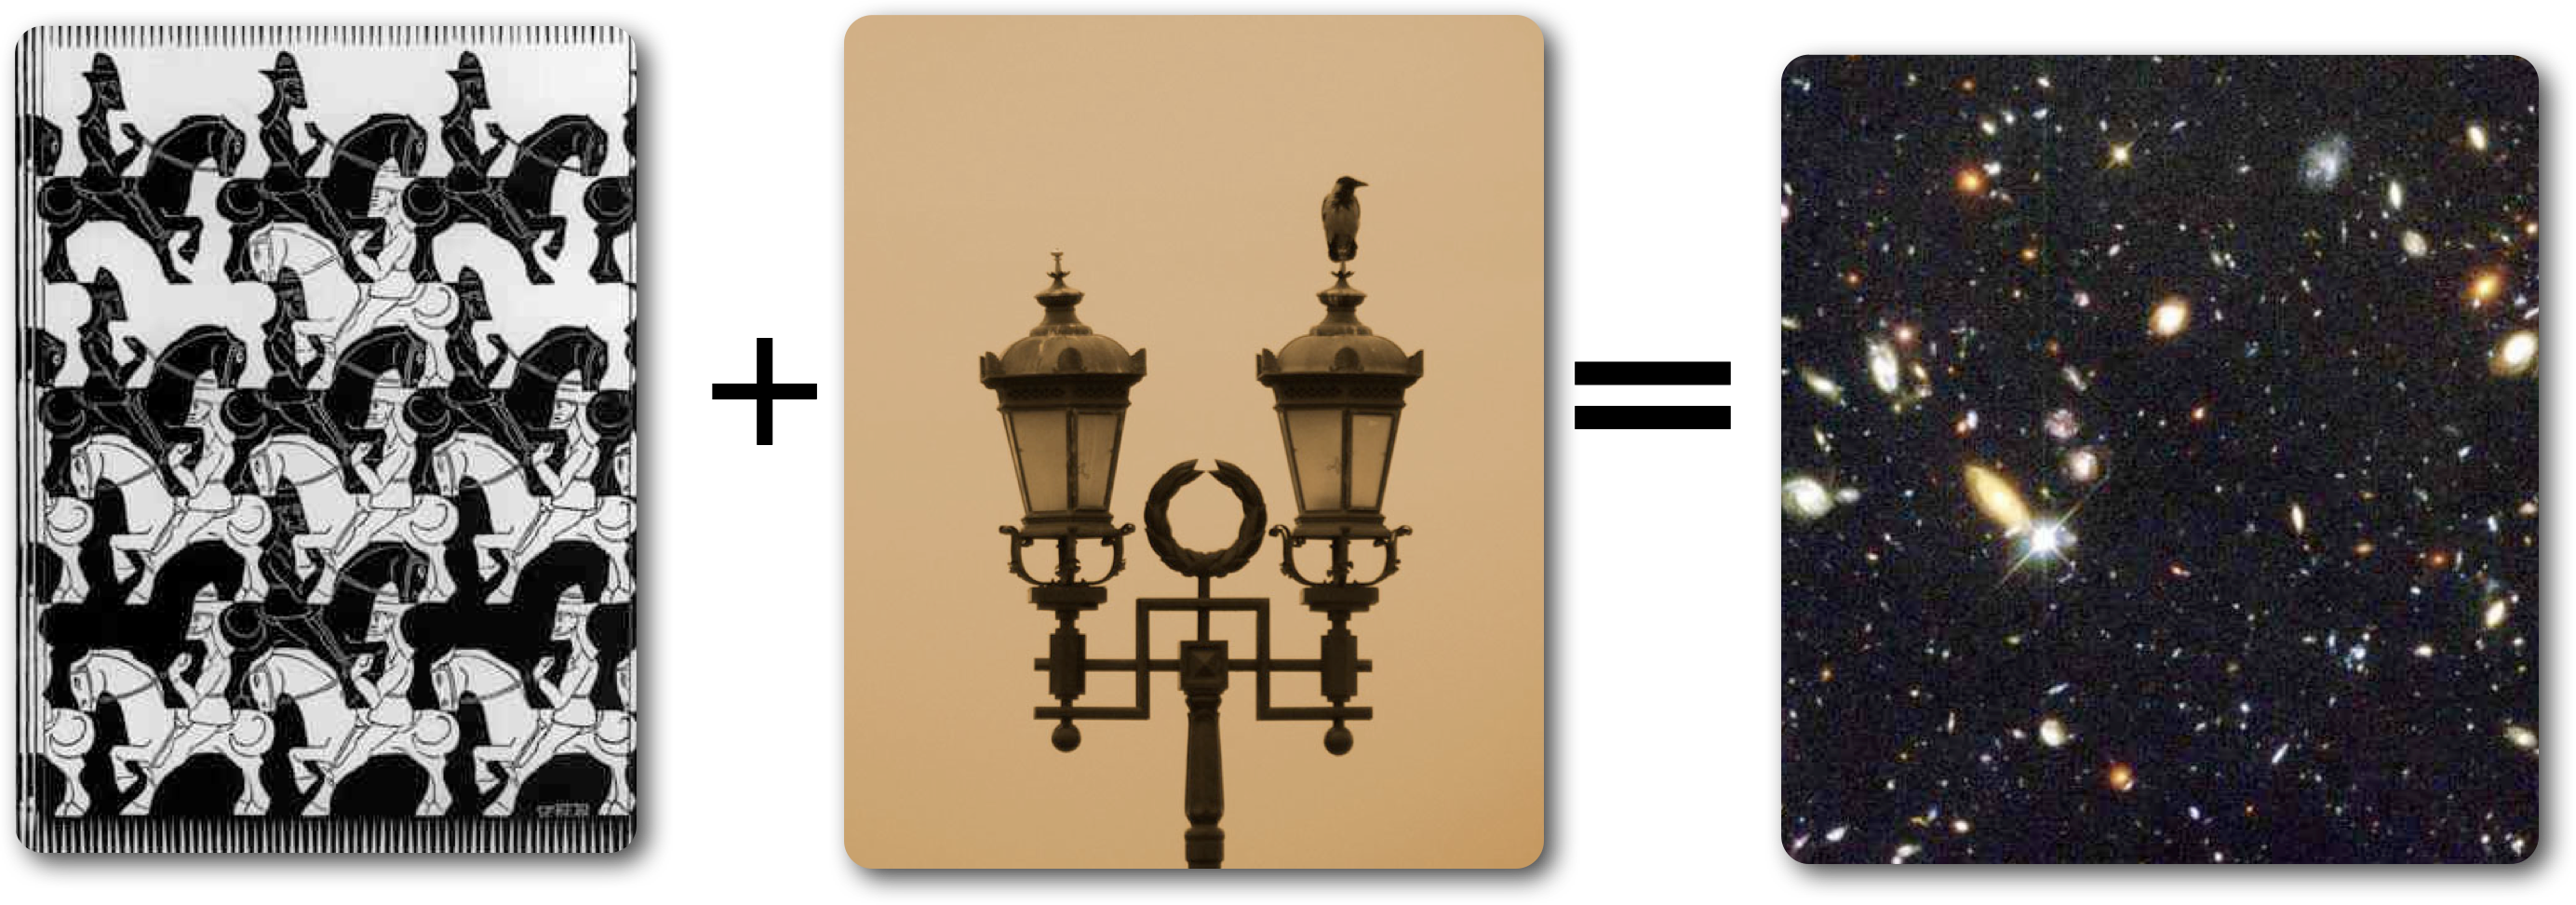
\includegraphics[scale=0.31]{formulaU.png}

\end{frame}


\begin{frame}{Doble o nada}

\begin{columns}
\column{0.5\textwidth}

\includegraphics[width=\textwidth,height=0.45\textheight,keepaspectratio]{doubleOrNothing.png}


\column{0.5\textwidth}


$\bullet$~¿Pero es realmente el neutrino su propia antipartícula?  

$\bullet$~Para demostrarlo, algunos físicos jugamos al juego de <<doble o nada>> en un casino subterráneo. 
 \end{columns}

\end{frame}

%%%%%

\begin{frame}{Desintegración doble beta sin neutrinos}

\begin{columns}
\column{0.5\textwidth}
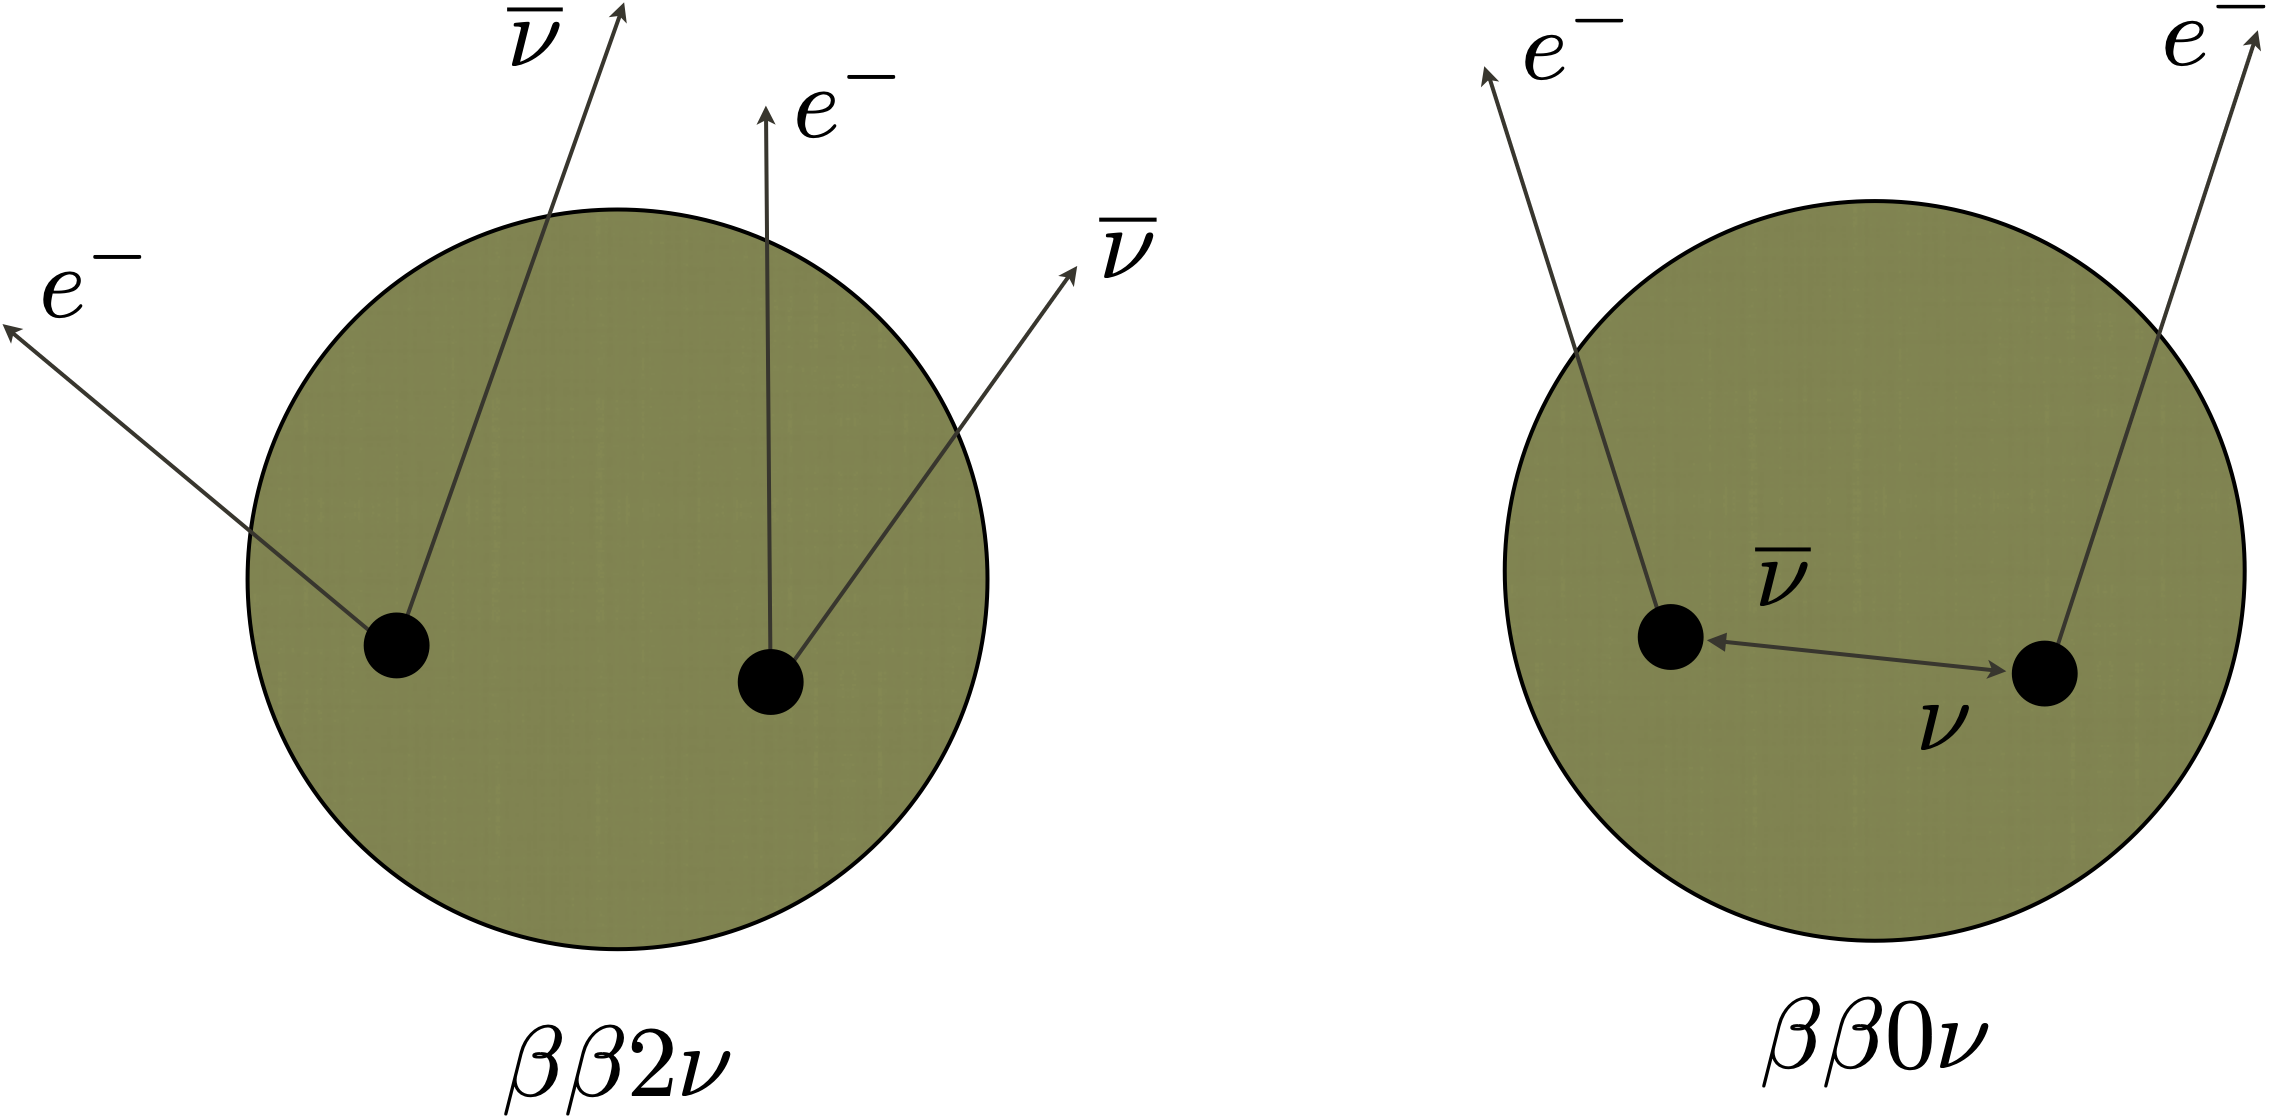
\includegraphics[width=\textwidth,height=0.45\textheight,keepaspectratio]{doubleBetaDecay.png}

\column{0.5\textwidth}


$\bullet$~La desintegración doble beta es una reacción muy rara, <<dos desintegraciones beta en cascada>>, pero conocida (y medida) por los físicos.   

$\bullet$~La desintegración doble beta \emph{sin neutrinos}, ($\beta\beta0\nu$) solo puede ocurrir si el neutrino es su propia antipartícula. Por lo tanto, detectarla demostraría que el neutrino es de Majorana y reforzaría mucho nuestra teoría sobre el origen del Universo. 


 \end{columns}

\end{frame}

%%%%%

\begin{frame}{Mucho más difícil que buscar una aguja en un pajar}

\begin{columns}
\column{0.5\textwidth}
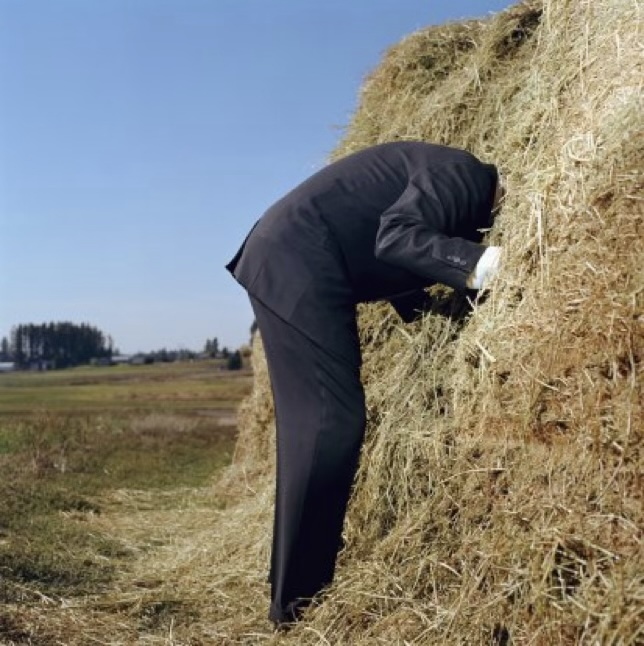
\includegraphics[width=\textwidth,height=0.35\textheight,keepaspectratio]{pajar.jpg}


\includegraphics[width=\textwidth,height=0.35\textheight,keepaspectratio]{beach.jpg}

\column{0.5\textwidth}


$\bullet$~La desintegración $\beta\beta0\nu$, si existe, es tan rara, que el ruido de fondo debido a la radioactividad natural de la Tierra hace que detectarla sea \emph{mucho más difícil} que encontrar una aguja en un pajar. De hecho, viene a ser como encontrar un grano de arena de color azul en la playa de La Concha\dots\ ¡si La Concha llegara hasta Bilbao!  

 \end{columns}

\end{frame}



%%%%
%\begin{frame}{Toda Odisea empieza con una idea estupenda}
%
%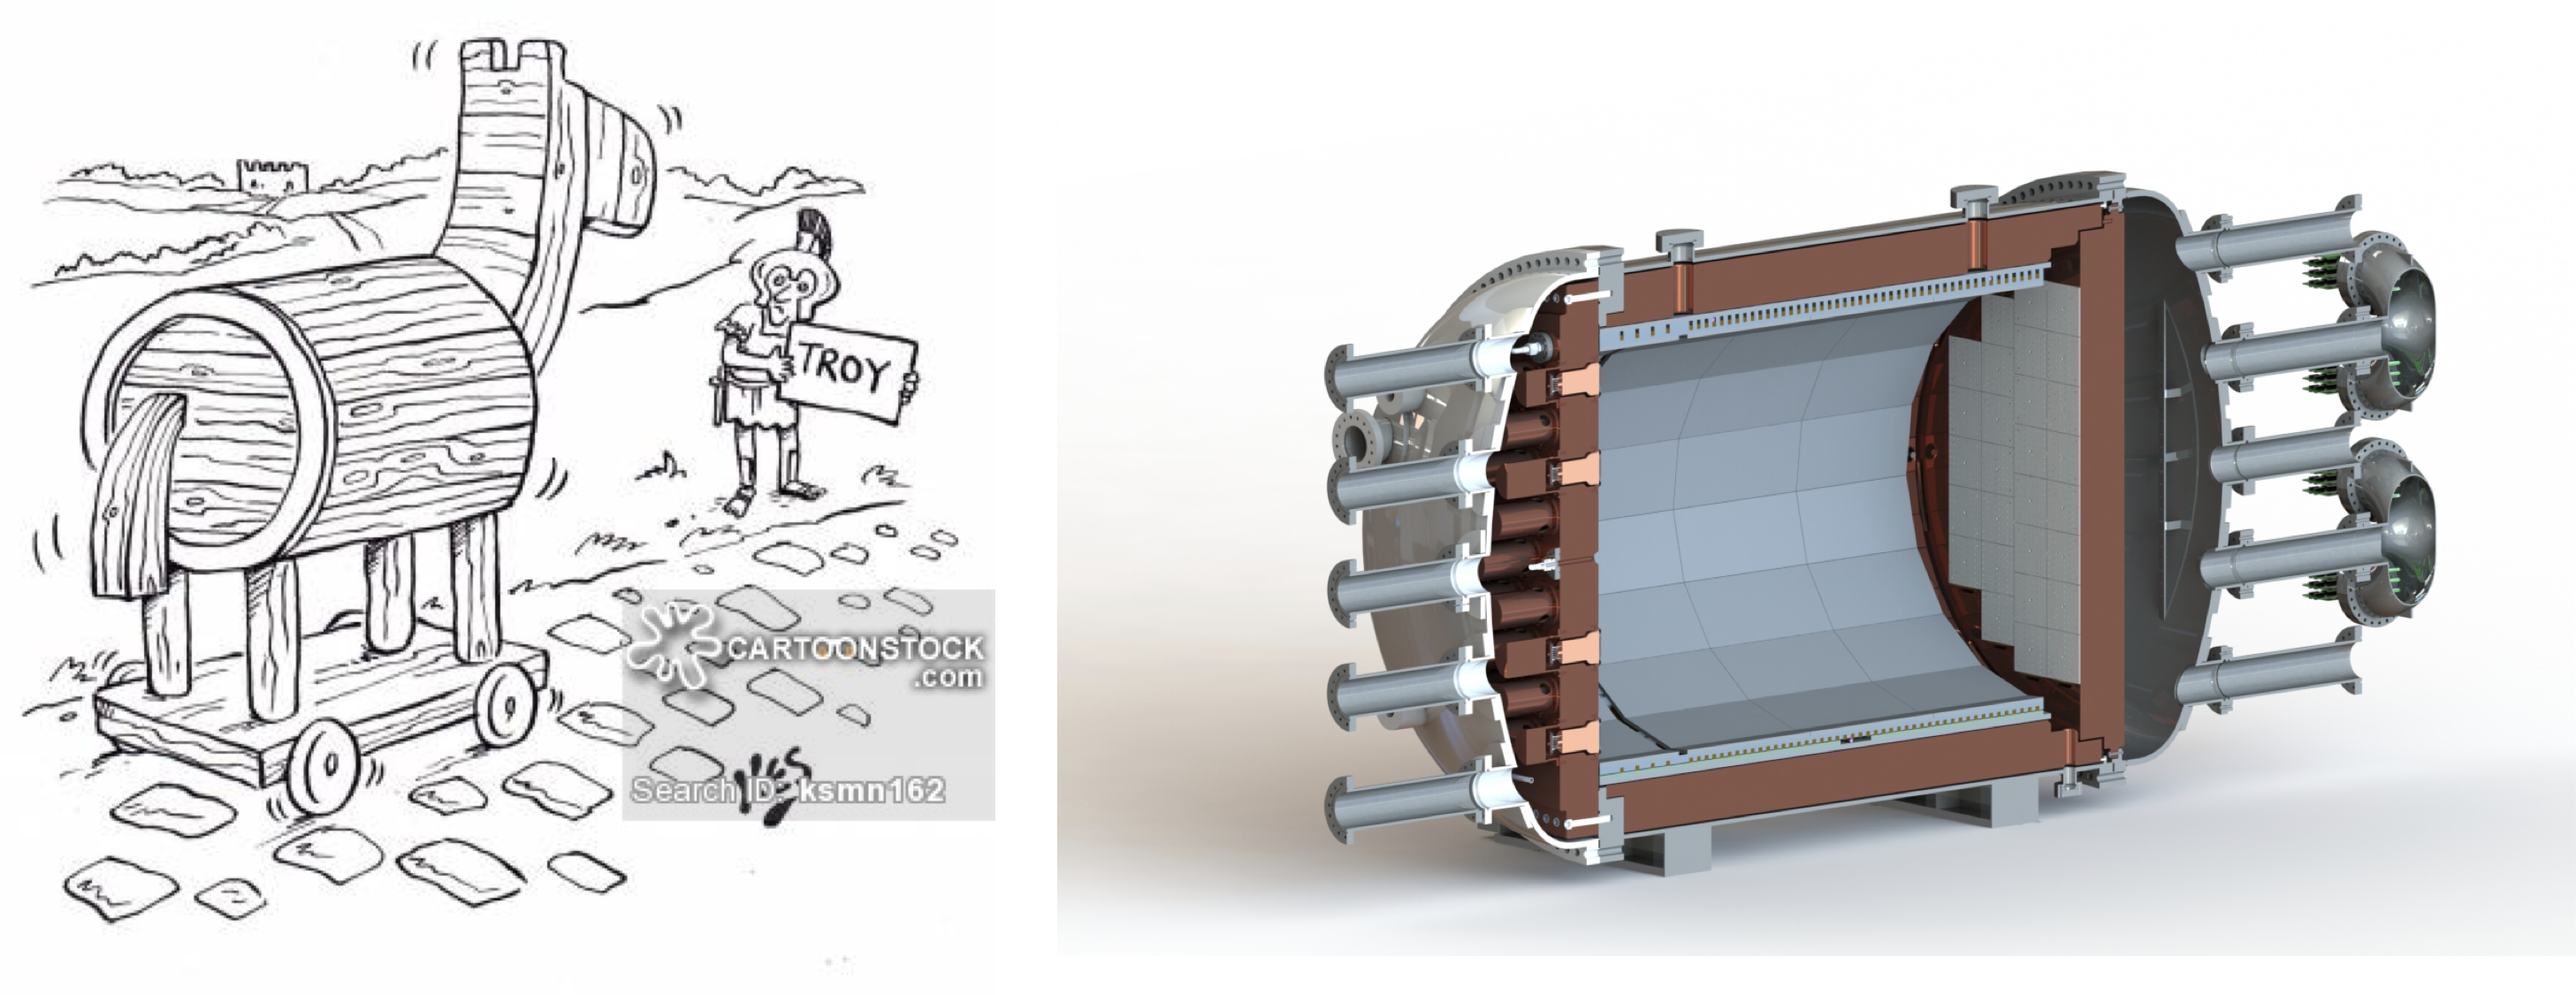
\includegraphics[scale=0.26]{odysseystart.png}
%
%\begin{columns}
%\column{0.50\textwidth}
%
%$\bullet$~Un nuevo artefacto para conquistar Troya.  
%
%\column{0.50\textwidth}
%$\bullet$~Un nuevo aparato para descubrir  $\beta\beta0\nu$.
%
%\end{columns}
%
%\end{frame}
%
%%%%
%\begin{frame}{Y total ignorancia de las complicaciones}
%
%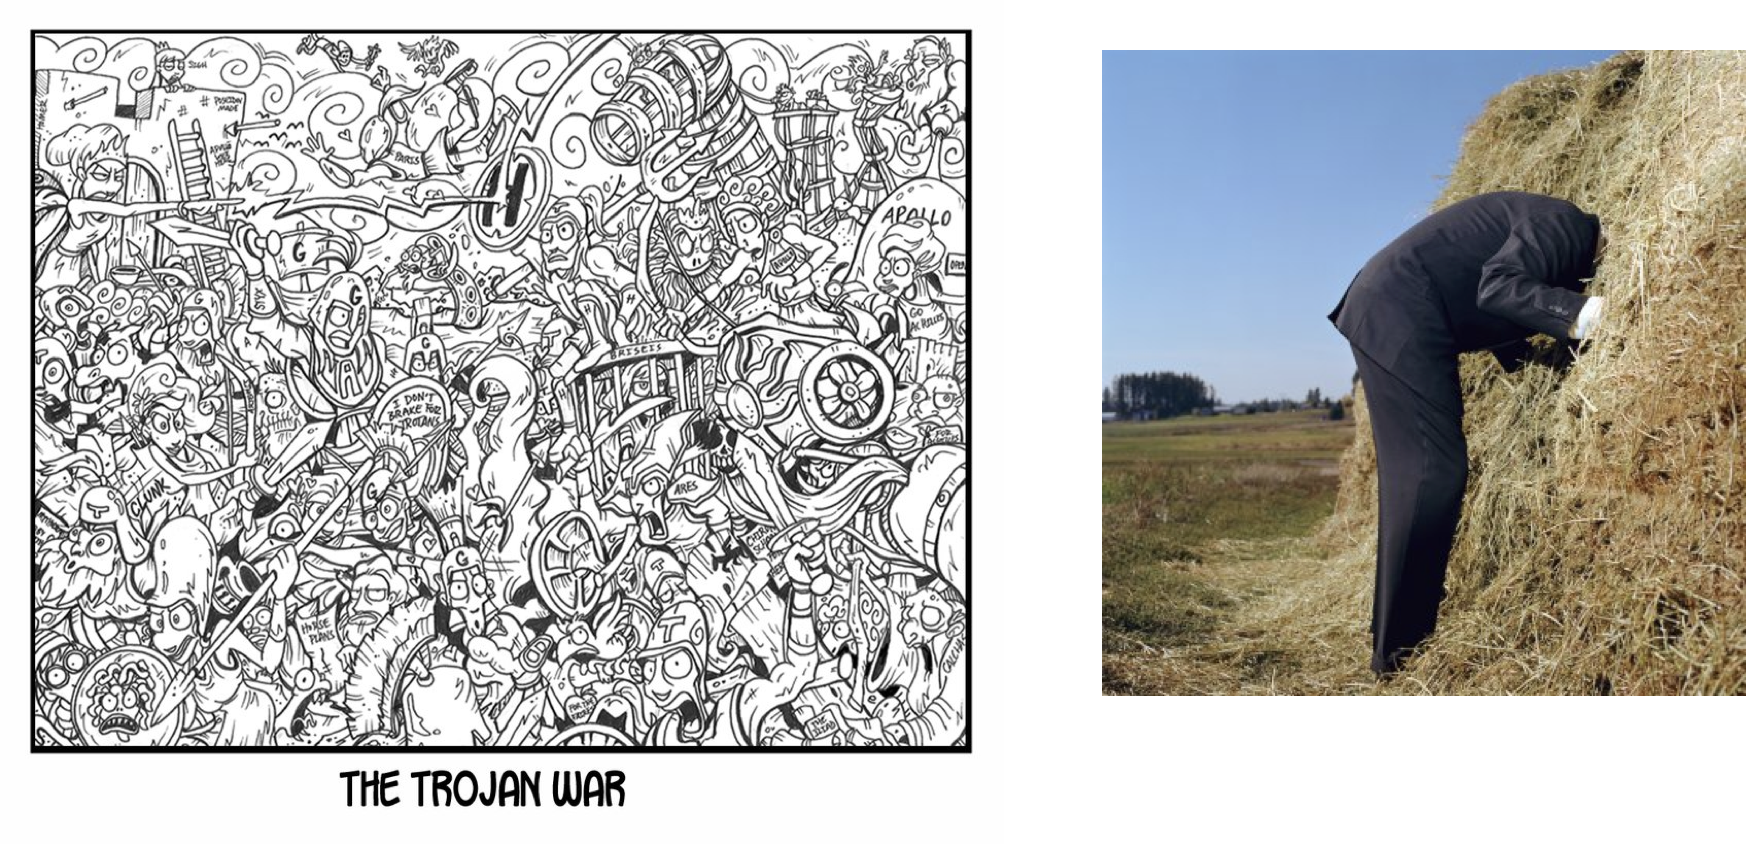
\includegraphics[scale=0.45]{complications.png}
%
%\end{frame}

\begin{frame}{NEXT (Neutrino Experiment with a Xenon TPC)}

\begin{columns}
\column{0.50\textwidth}
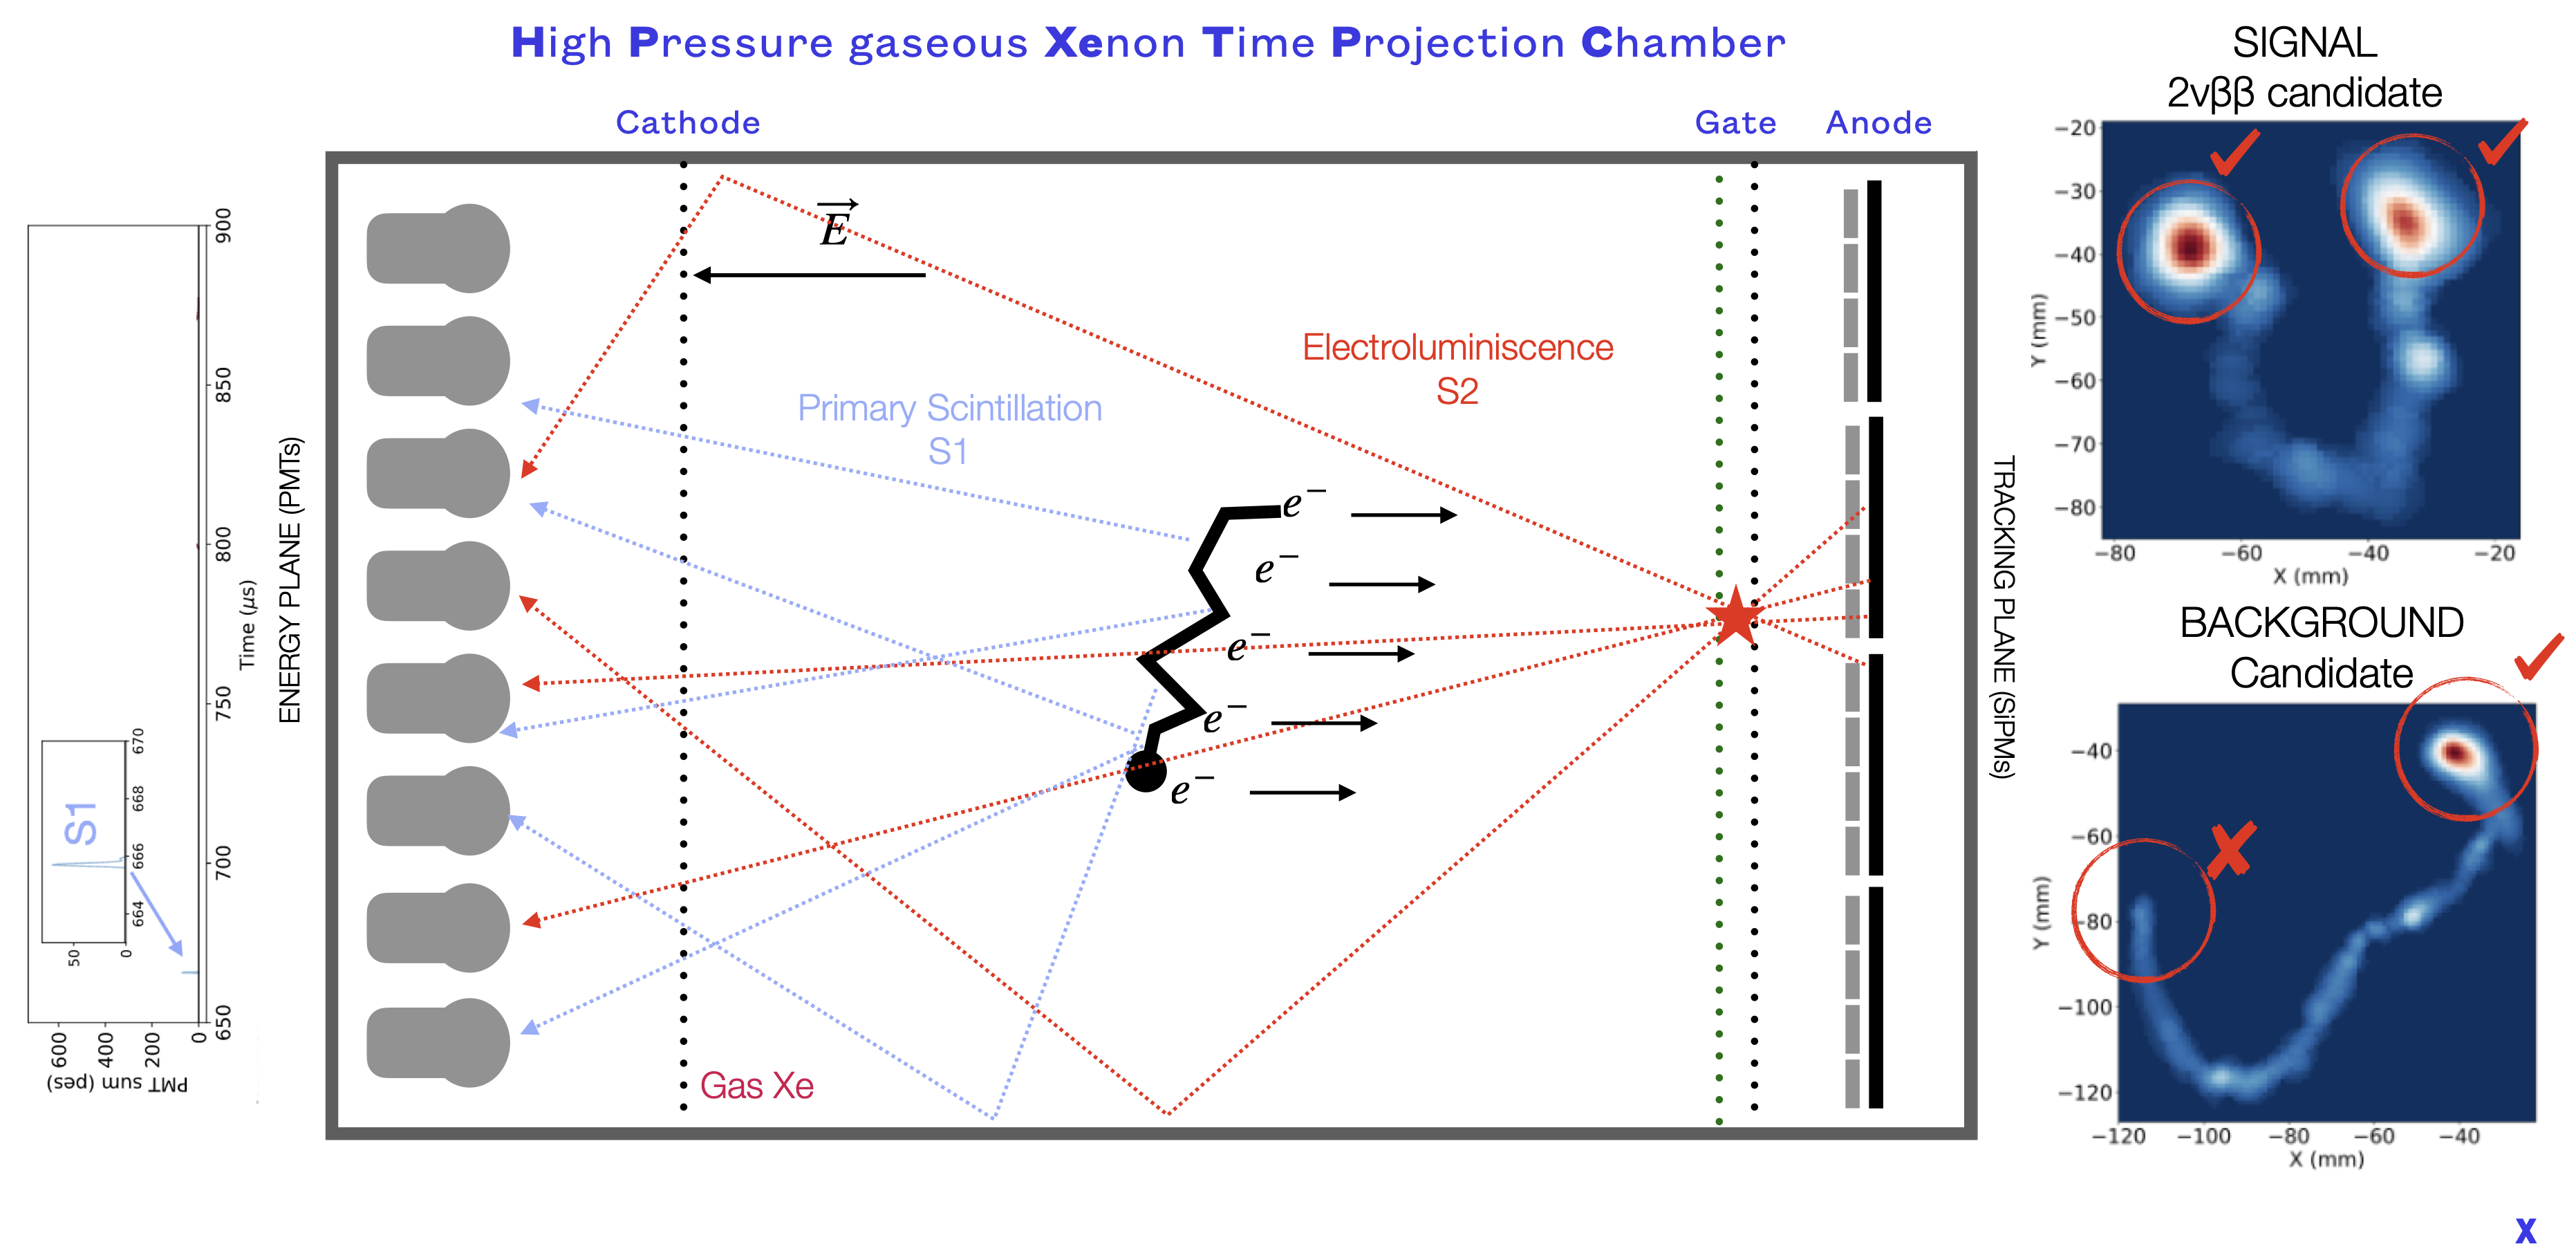
\includegraphics[width=\textwidth,height=0.45\textheight,keepaspectratio]{nexttraum.png}


 \column{0.50\textwidth}
$\bullet$~NEXT es una cámara llena de xenón a alta presión, equipada con sensores muy precisos y muy radiopuros. El isótopo ${}^{136}$Xe puede desintegrarse vía $\beta\beta0\nu$ emitiendo dos electrones.

$\bullet$~NEXT mide con gran fidelidad la señal de esos electrones. Eso permite separar la escasa señal (un suceso cada diez años con el detector actual; uno al año con diez veces más masa) del gigantesco ruido de fondo (millones de sucesos al año).


\end{columns}
\end{frame}

\begin{frame}{Primeros prototipos}

\begin{columns}
\column{0.60\textwidth}
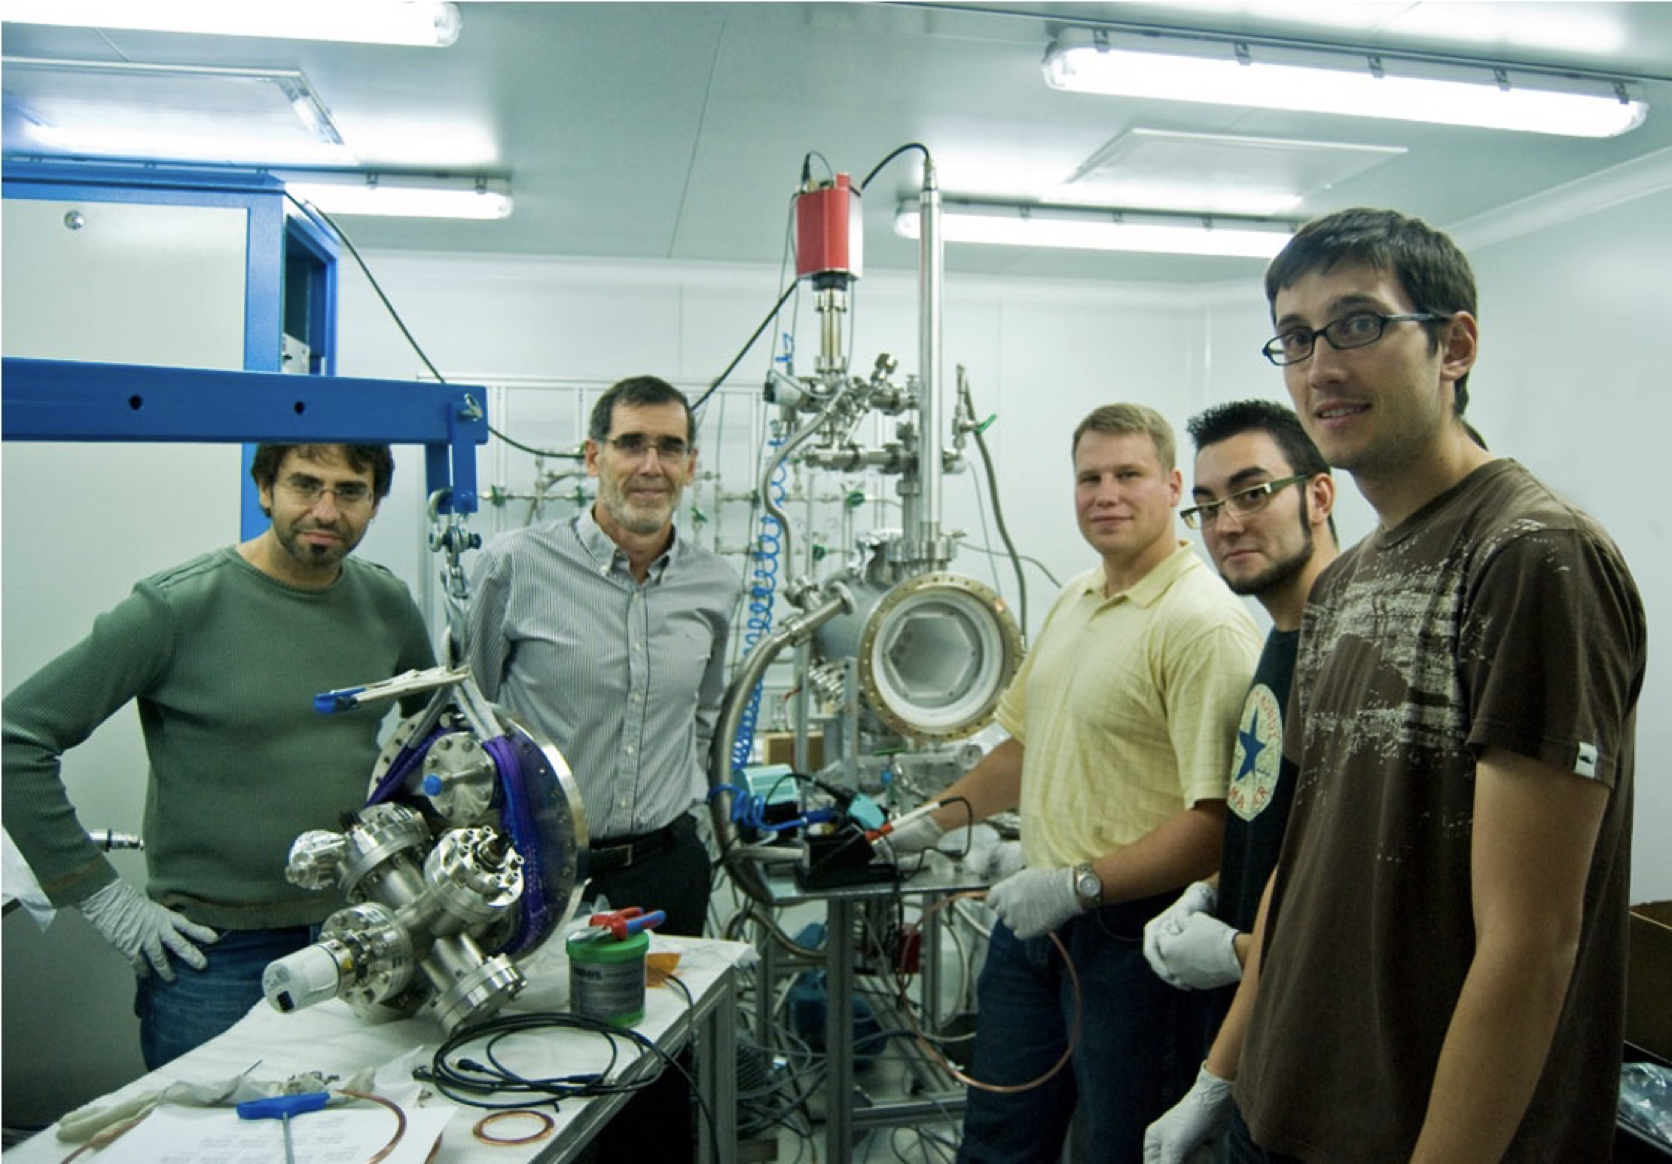
\includegraphics[scale=0.28]{next-demo.png}


 \column{0.40\textwidth}
$\bullet$~Entre 2009 y 2015 operamos dos prototipos: NEXT-DBDM en Berkeley y NEXT-DEMO en Valencia. El \emph{Traum} (sueño) se hizo \emph{Wirklichkeit} (realidad).

\end{columns}
\end{frame}


\begin{frame}{NEXT-White}

\begin{columns}
\column{0.60\textwidth}
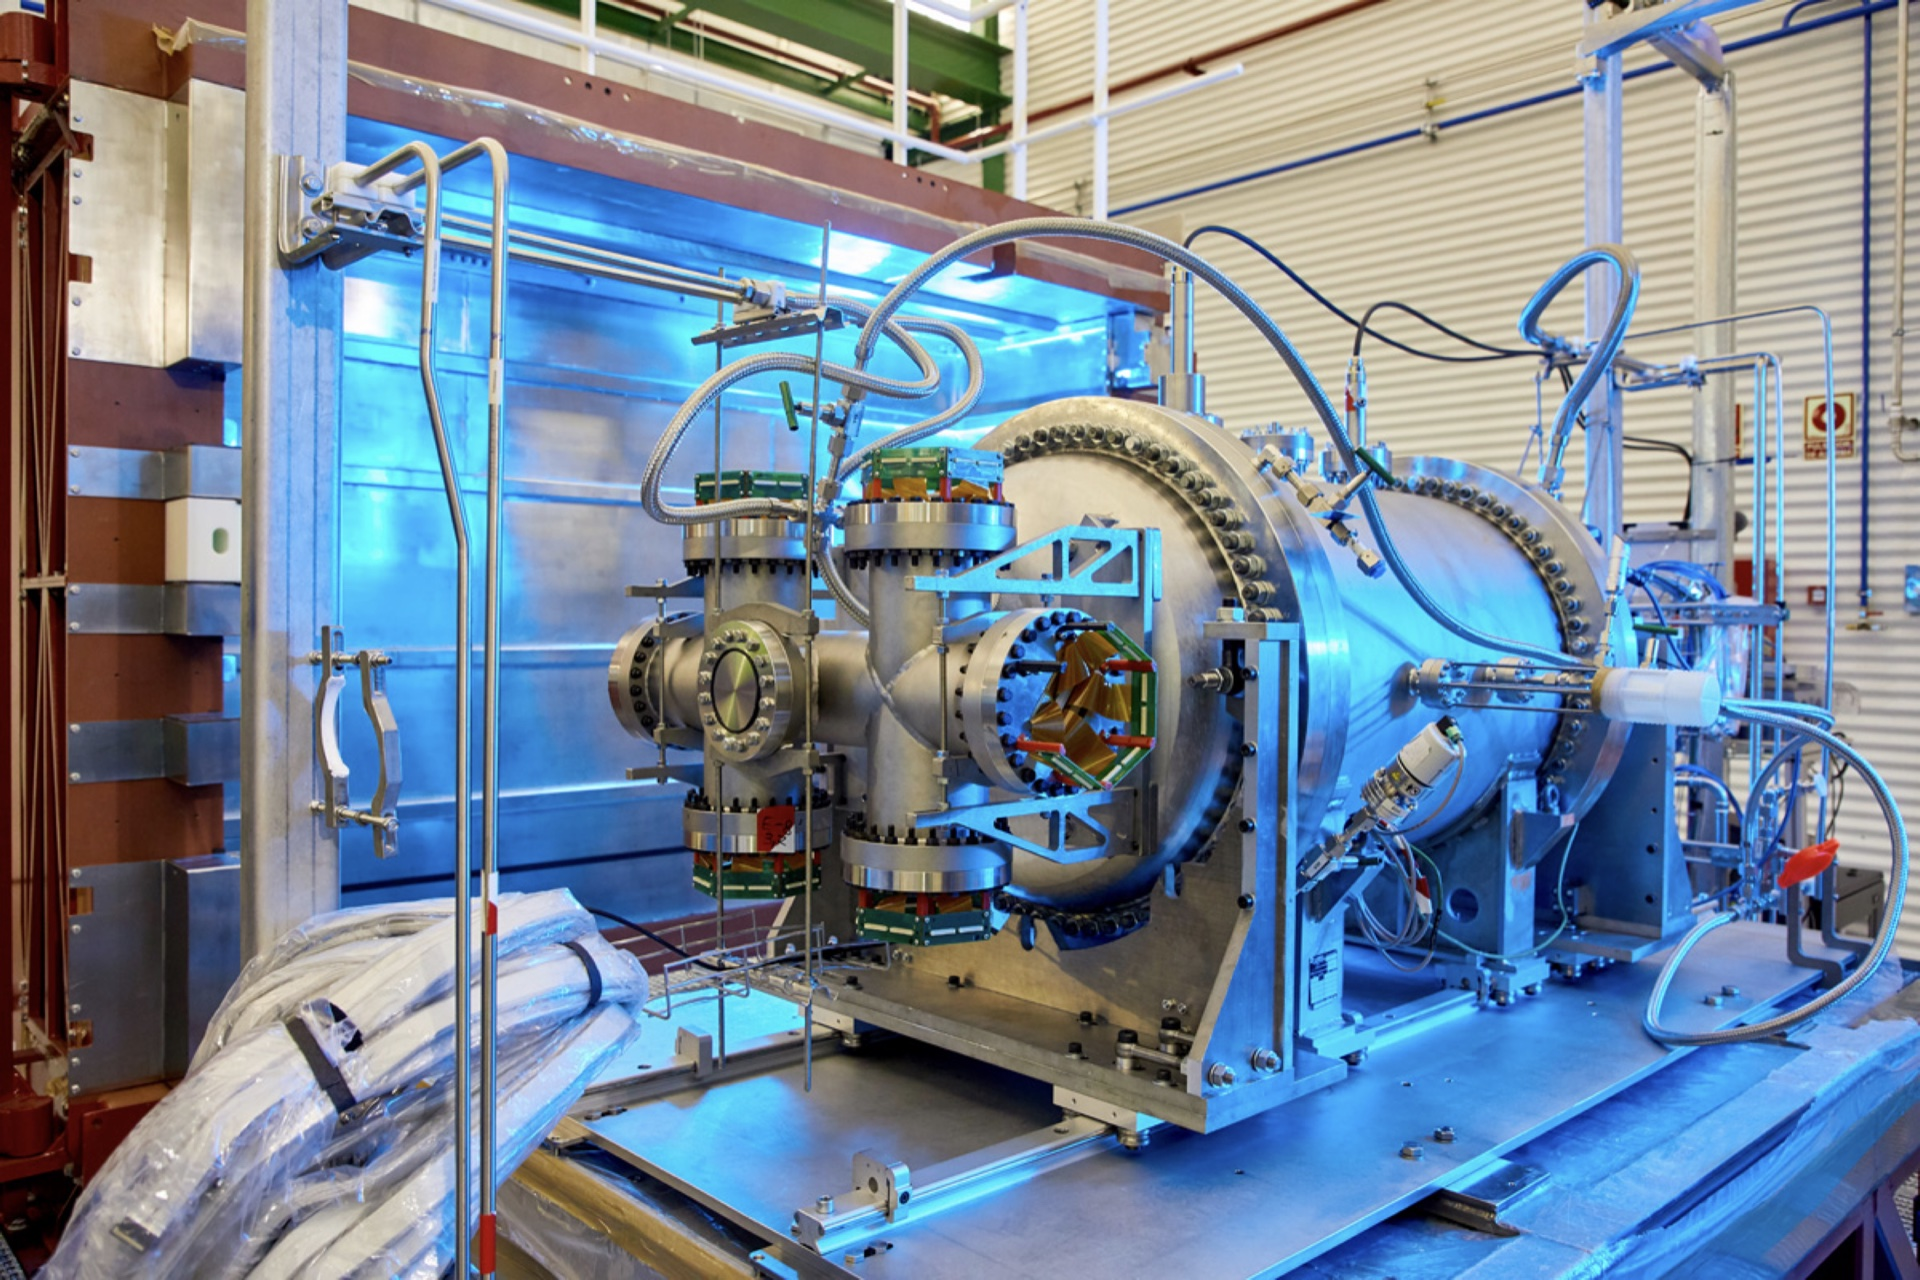
\includegraphics[width=\textwidth,height=0.75\textheight,keepaspectratio]{white.jpg}

 \column{0.40\textwidth}
$\bullet$~NEXT-White, bautizado en memoria de James White, fue el primer detector radiopuro de NEXT. Operó en el Laboratorio Subterráneo de Canfranc de 2016 a 2022.

\end{columns}
\end{frame}

\begin{frame}{El castillo de plomo}

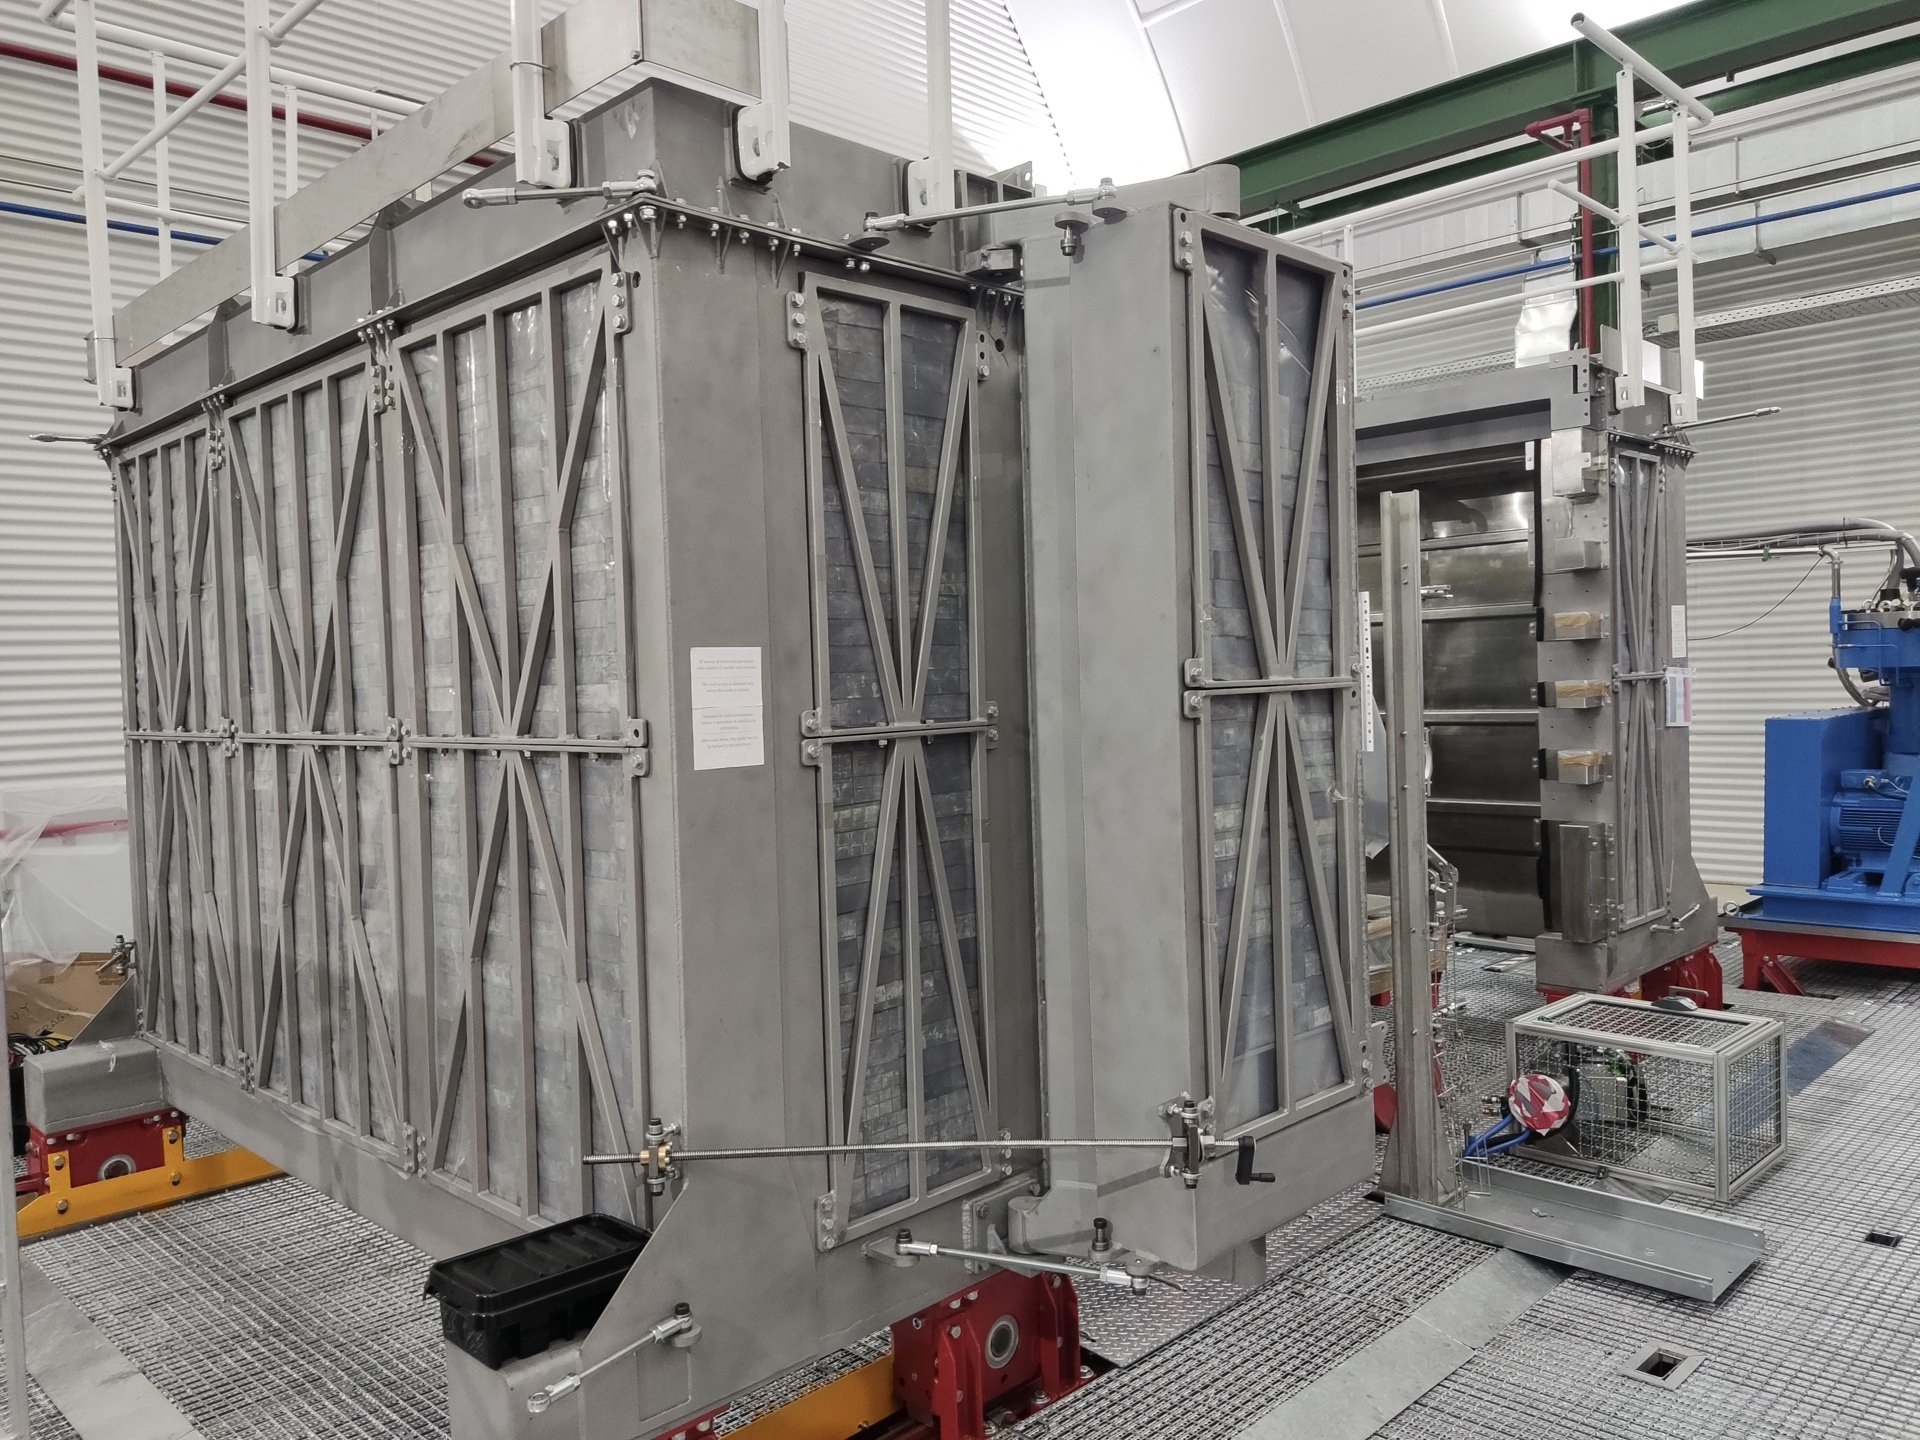
\includegraphics[width=\textwidth,height=0.78\textheight,keepaspectratio]{leadCastle.jpg}

\end{frame}


\begin{frame}{Vasija a presión y blindaje interno de cobre}
\begin{columns}
\column{0.50\textwidth}
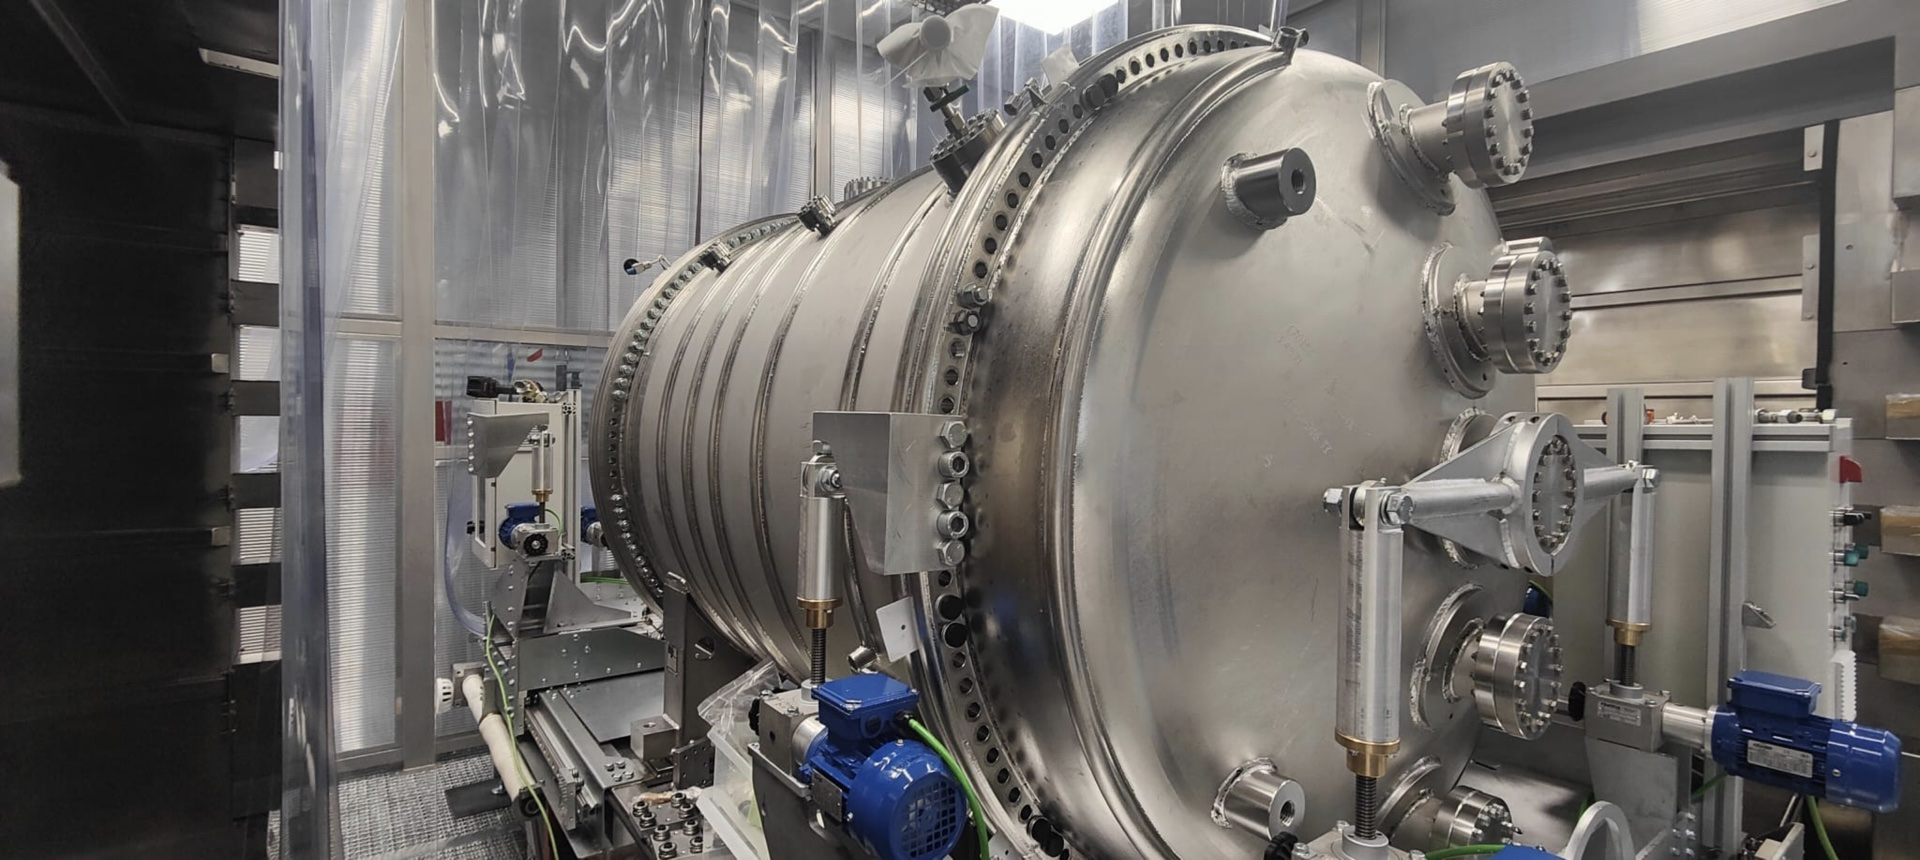
\includegraphics[width=\textwidth,height=0.75\textheight,keepaspectratio]{next100pv.jpg}

\column{0.50\textwidth}
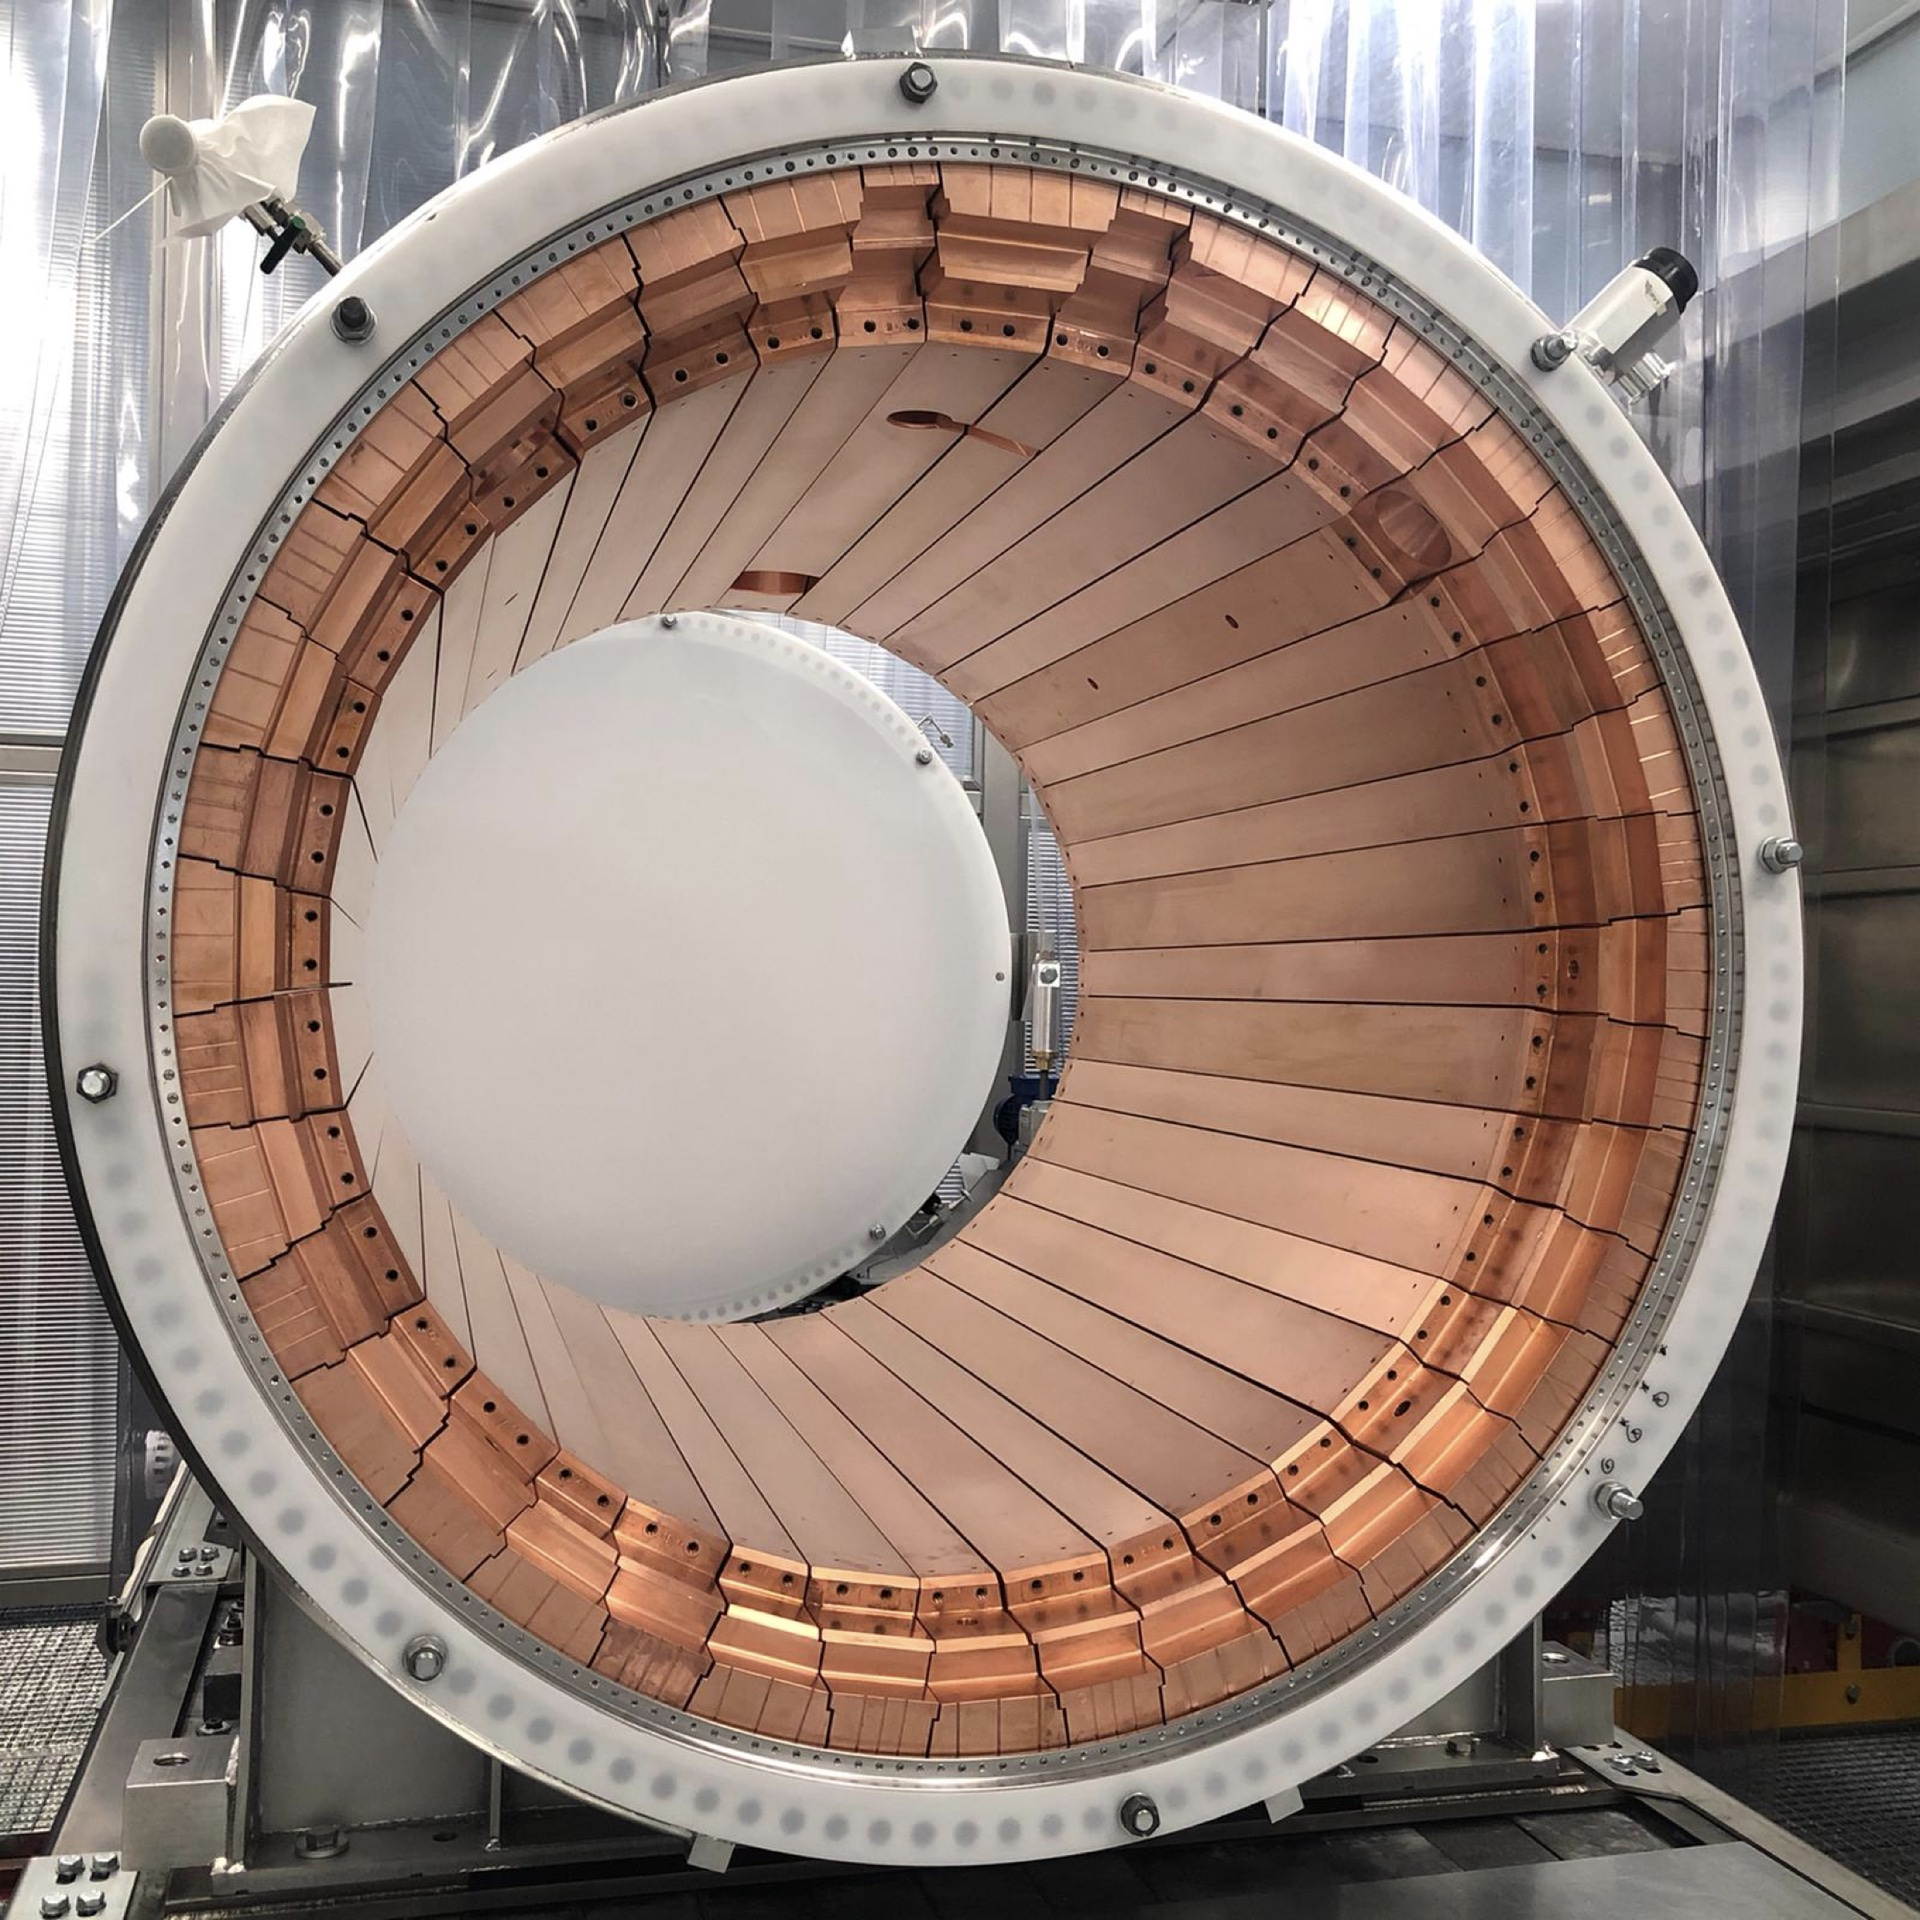
\includegraphics[width=\textwidth,height=0.75\textheight,keepaspectratio]{innercopper.jpg}

\end{columns}

\end{frame}

%\begin{frame}{PMTs \& SiPMs}
%
%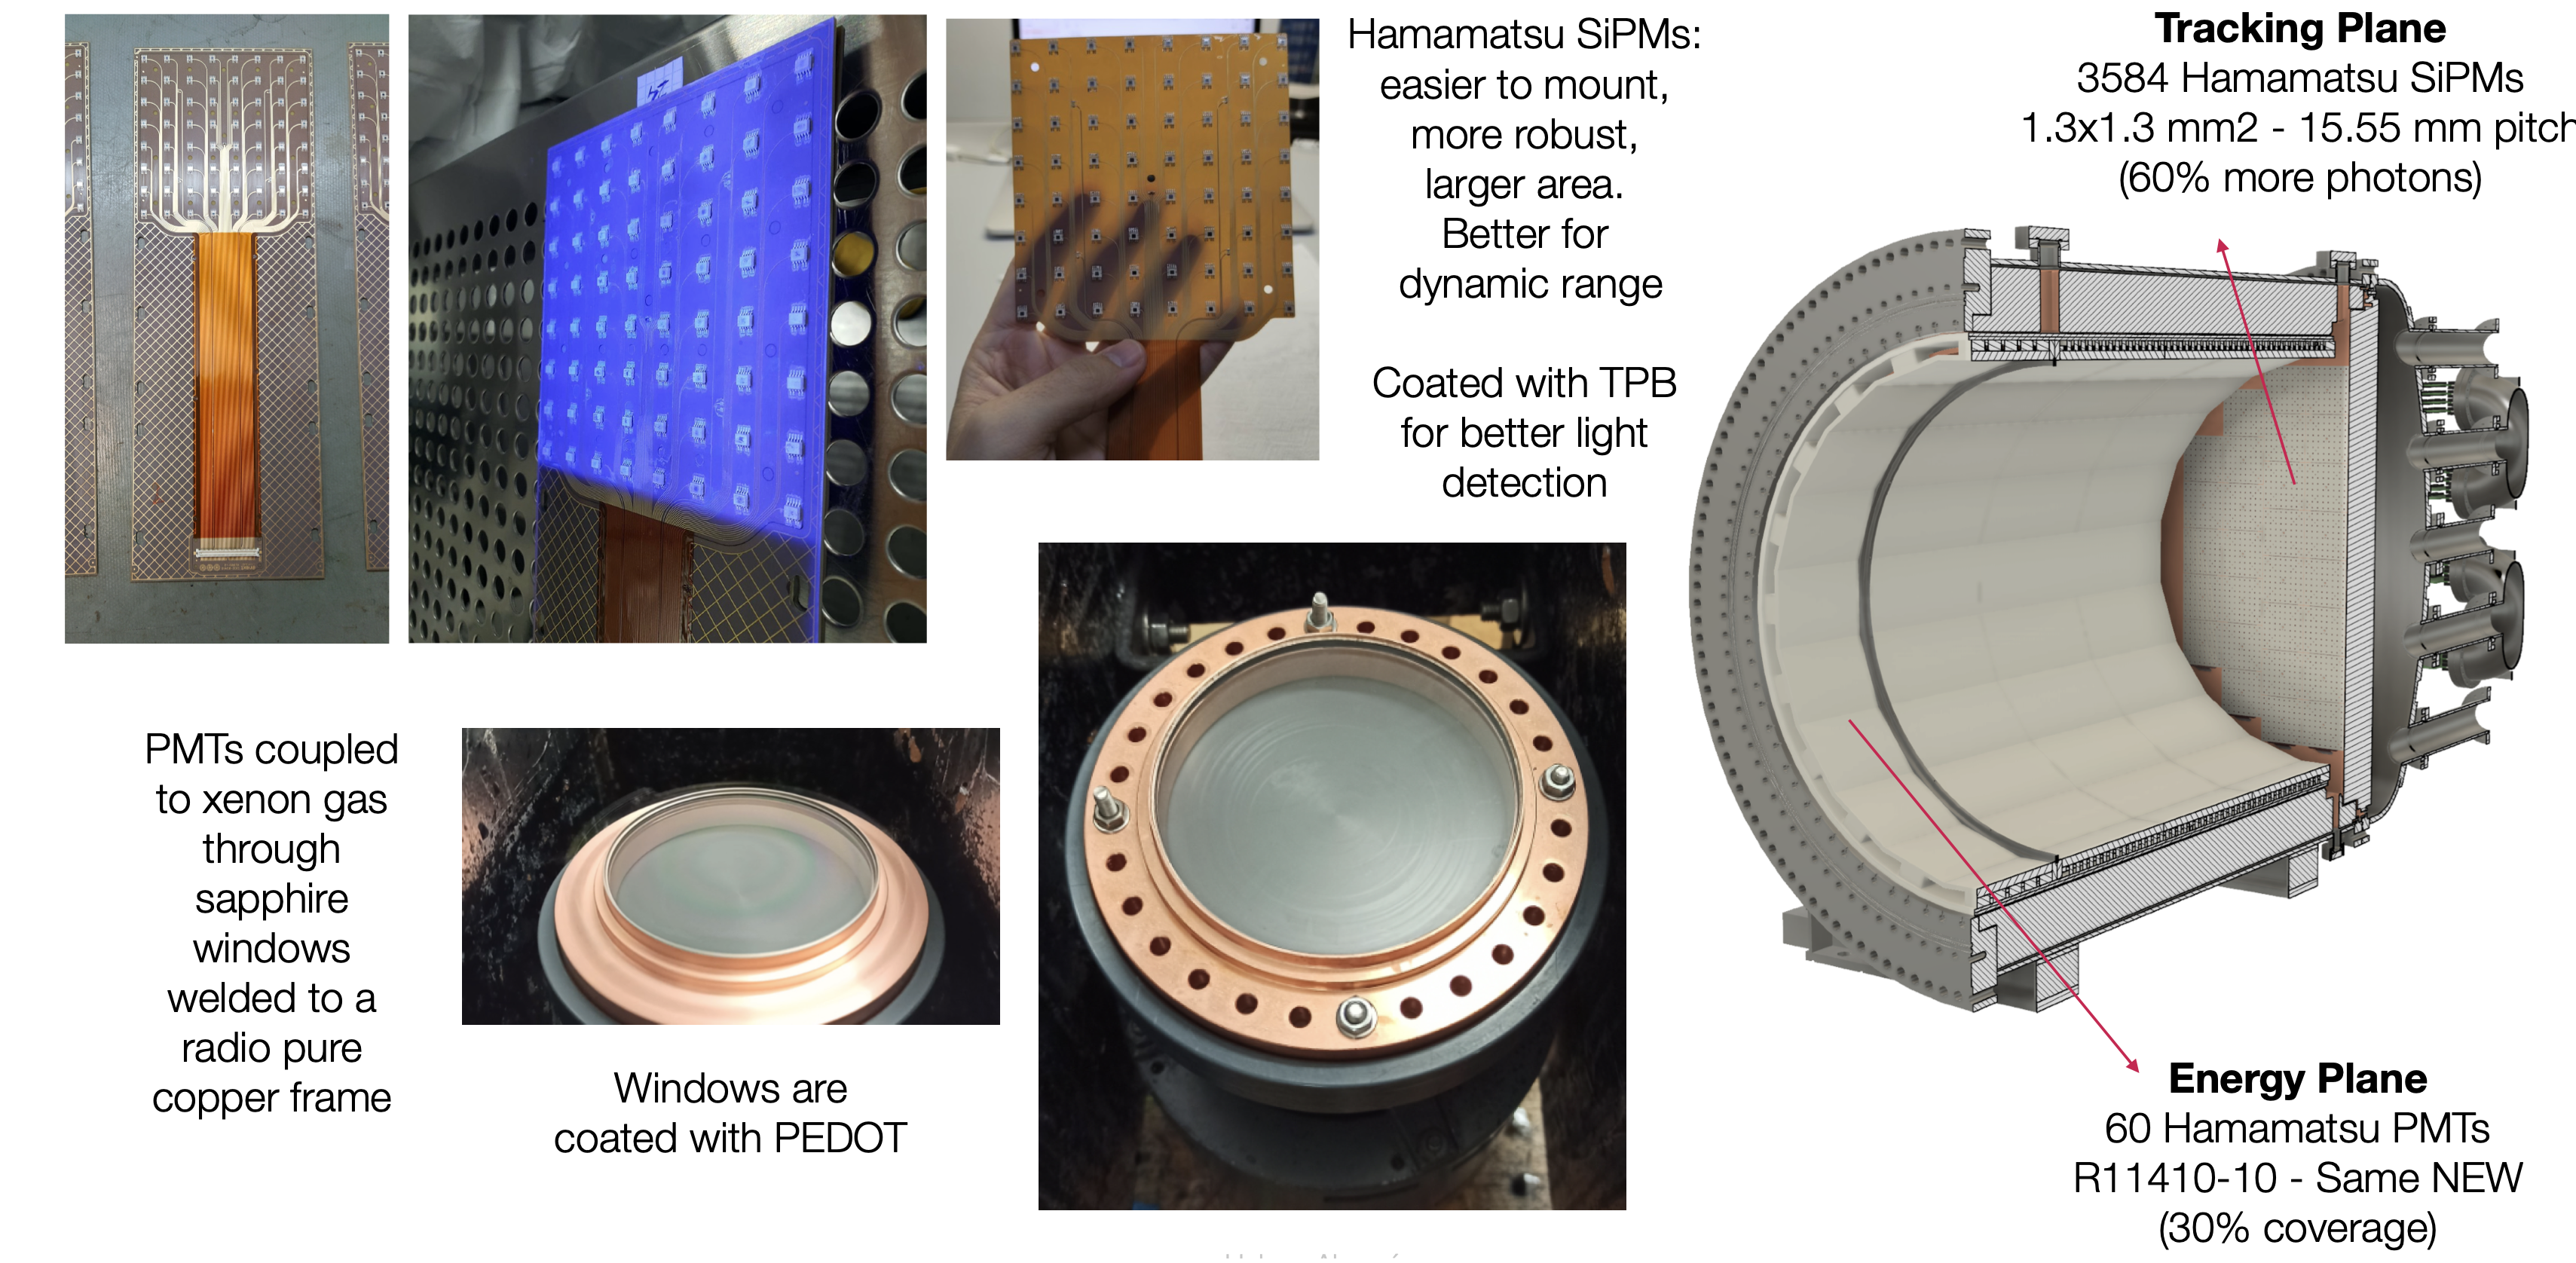
\includegraphics[scale=0.23]{sipmandpmts.png}
%
%\end{frame}

%%%%

\begin{frame}{Plano de energía y plano de trazas}

\begin{columns}
\column{0.50\textwidth}
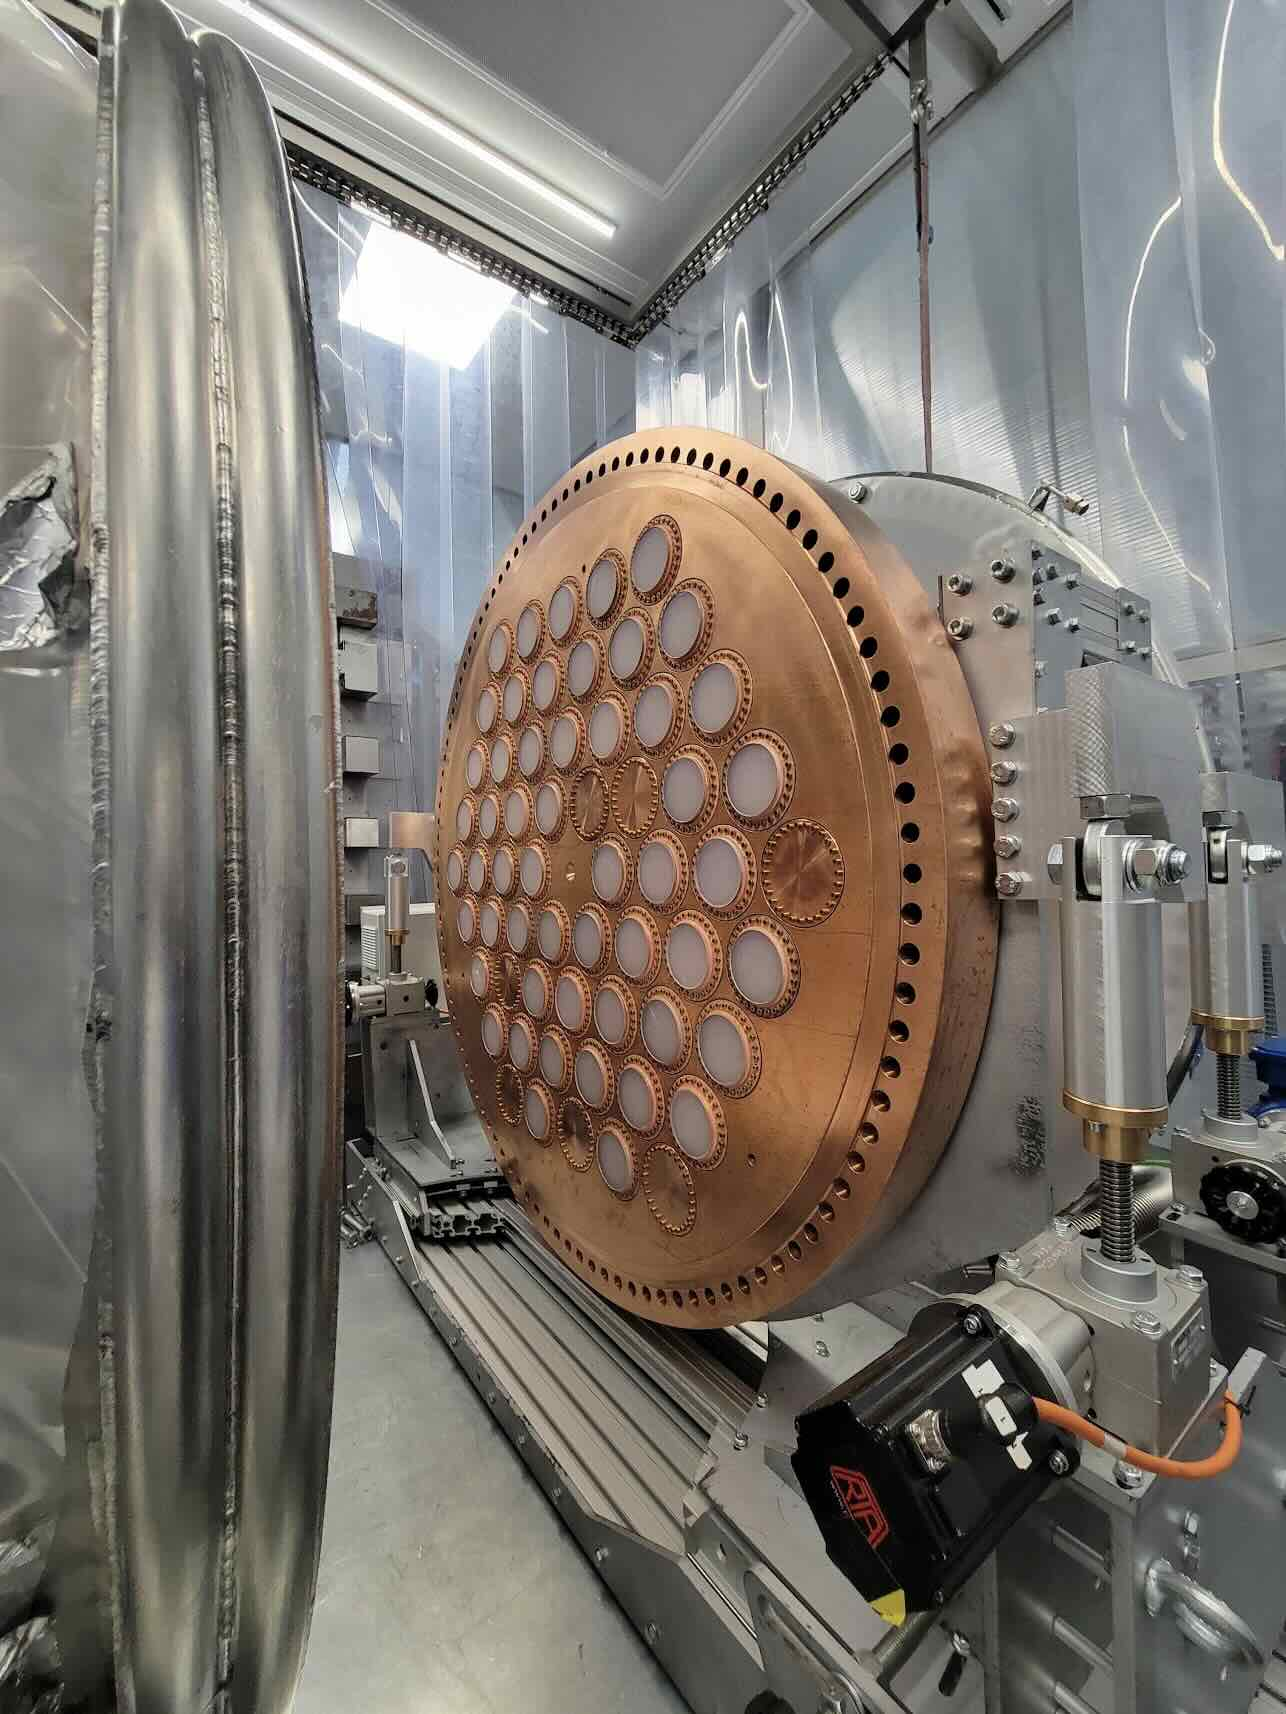
\includegraphics[scale=0.12]{n100-pmt.jpeg}
\column{0.50\textwidth}
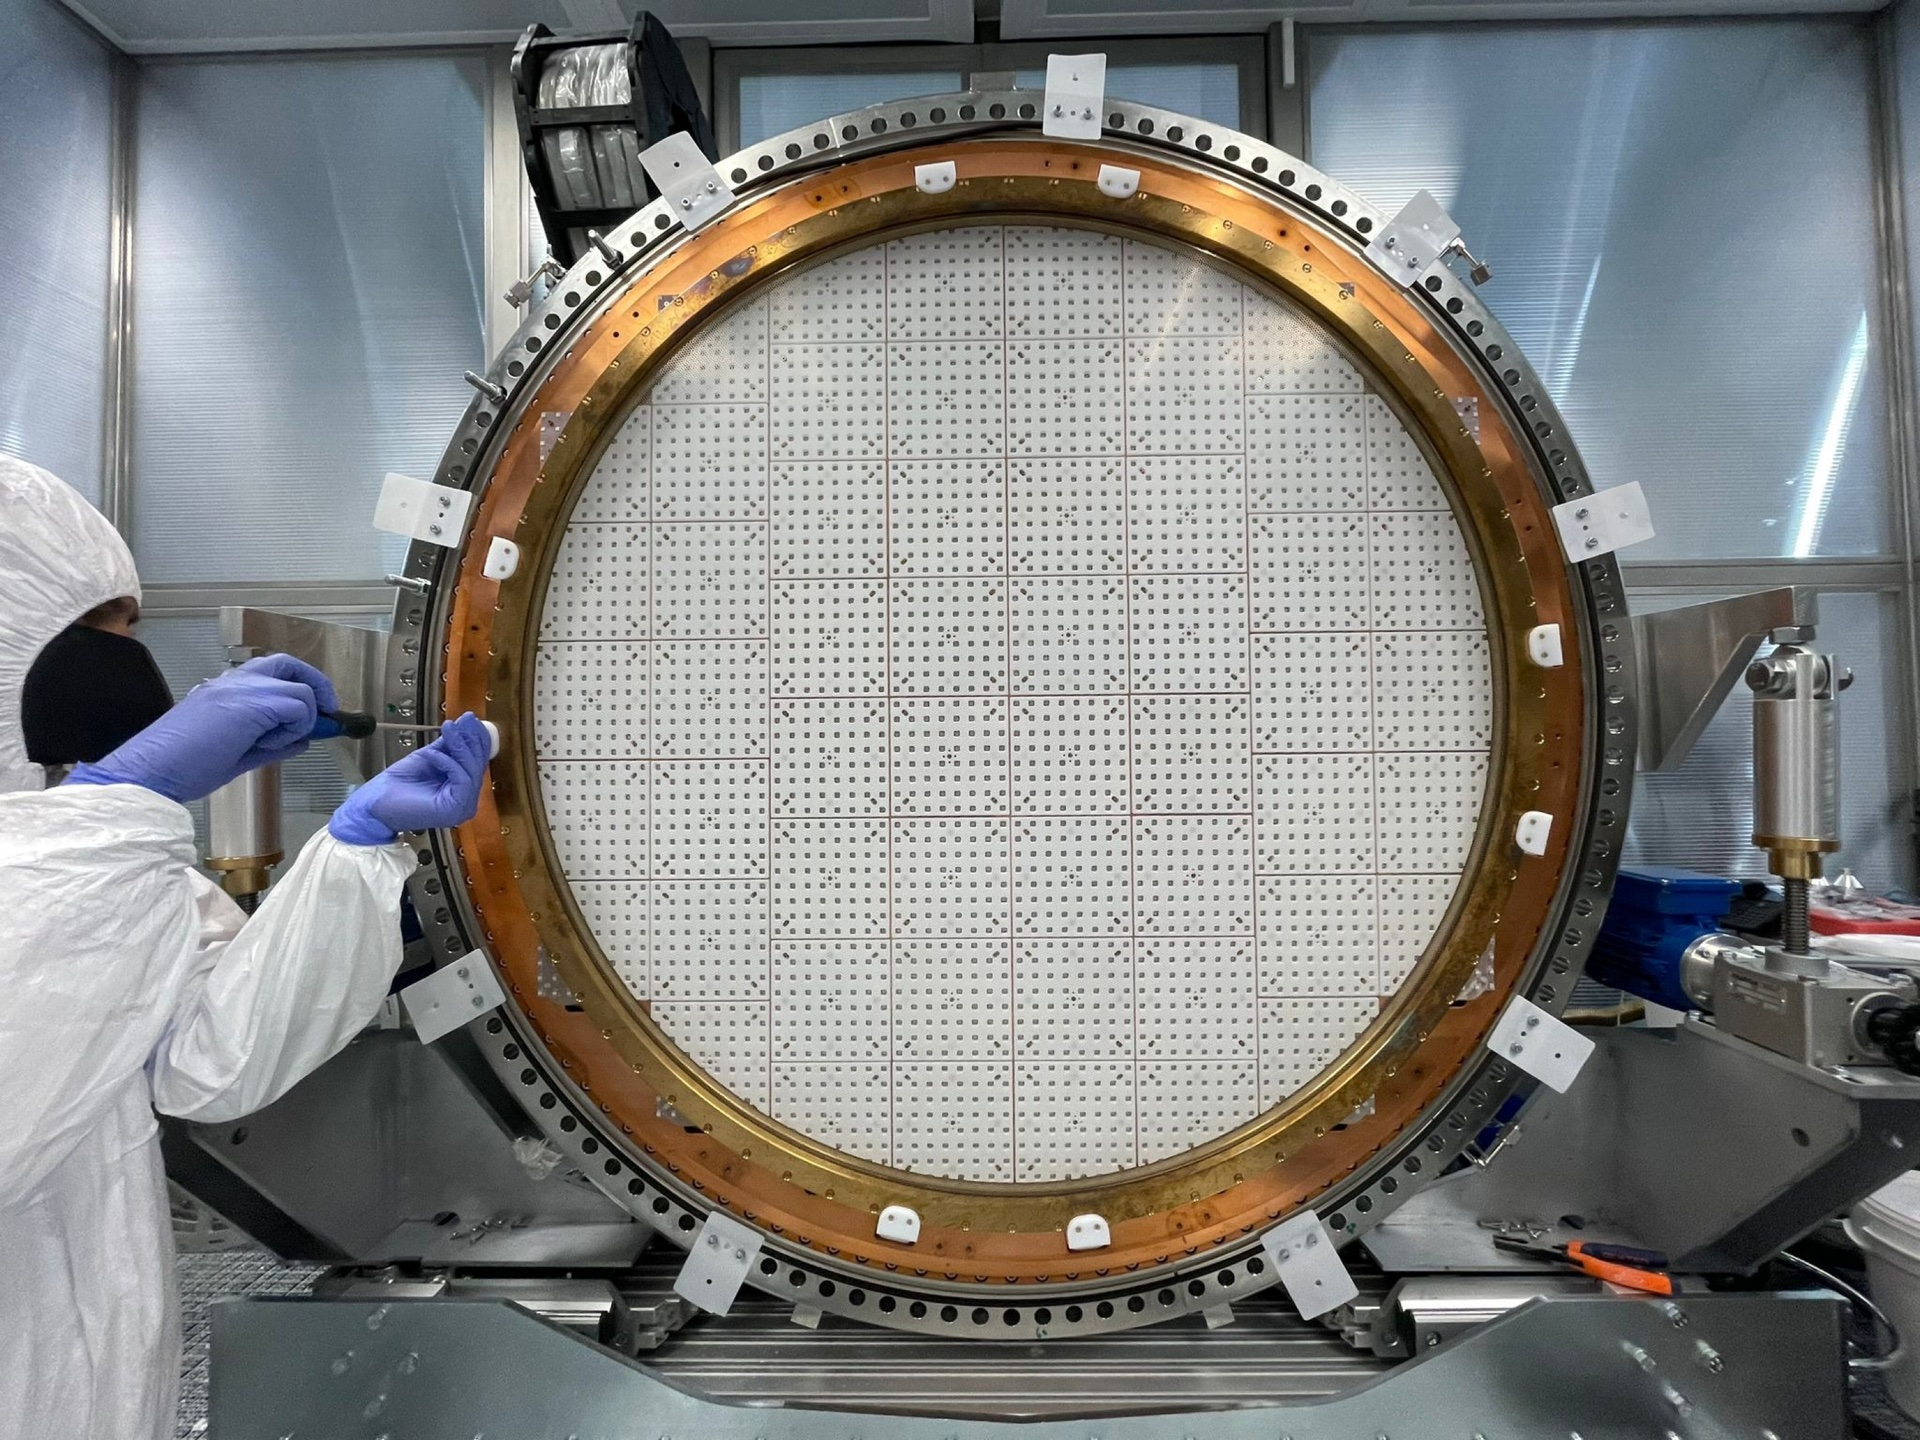
\includegraphics[width=\textwidth,height=0.70\textheight,keepaspectratio]{trackingplaneNext100.jpg} \\
\vspace{0.3em}
\begin{center}{\tiny JINST 19 P02007}\end{center}


\end{columns}
\end{frame}


%%%%%
\begin{frame}{Jaula de campo y tubo de luz}

\begin{columns}
\column{0.50\textwidth}
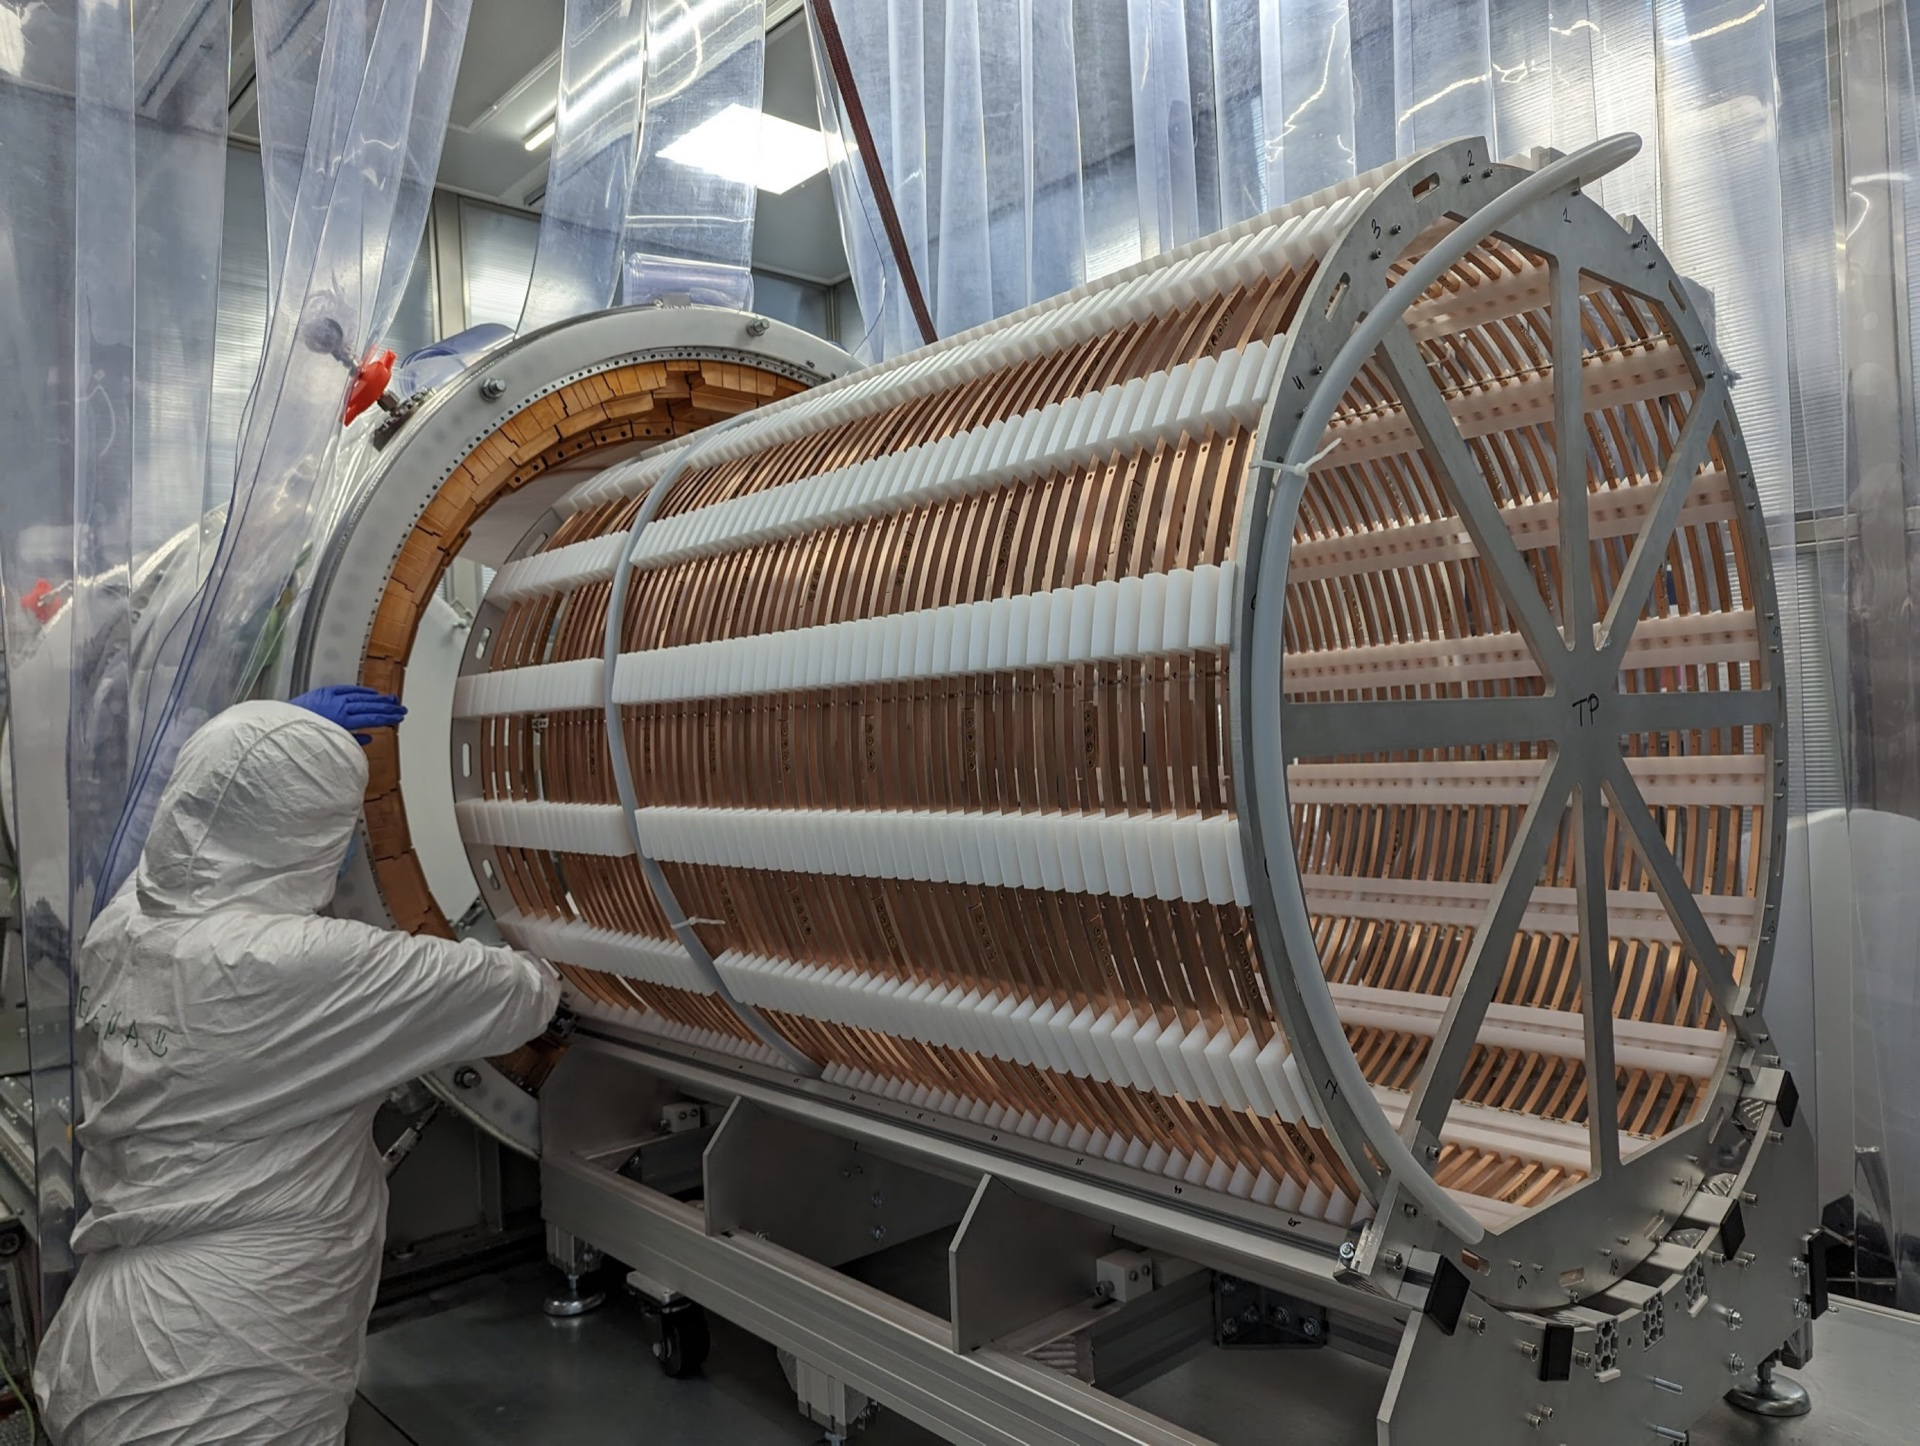
\includegraphics[width=\textwidth,height=0.70\textheight,keepaspectratio]{fieldcage.jpg}\\
\vspace{0.3em}
\begin{center}{\tiny arXiv 2505.01002}\end{center}

\column{0.50\textwidth}
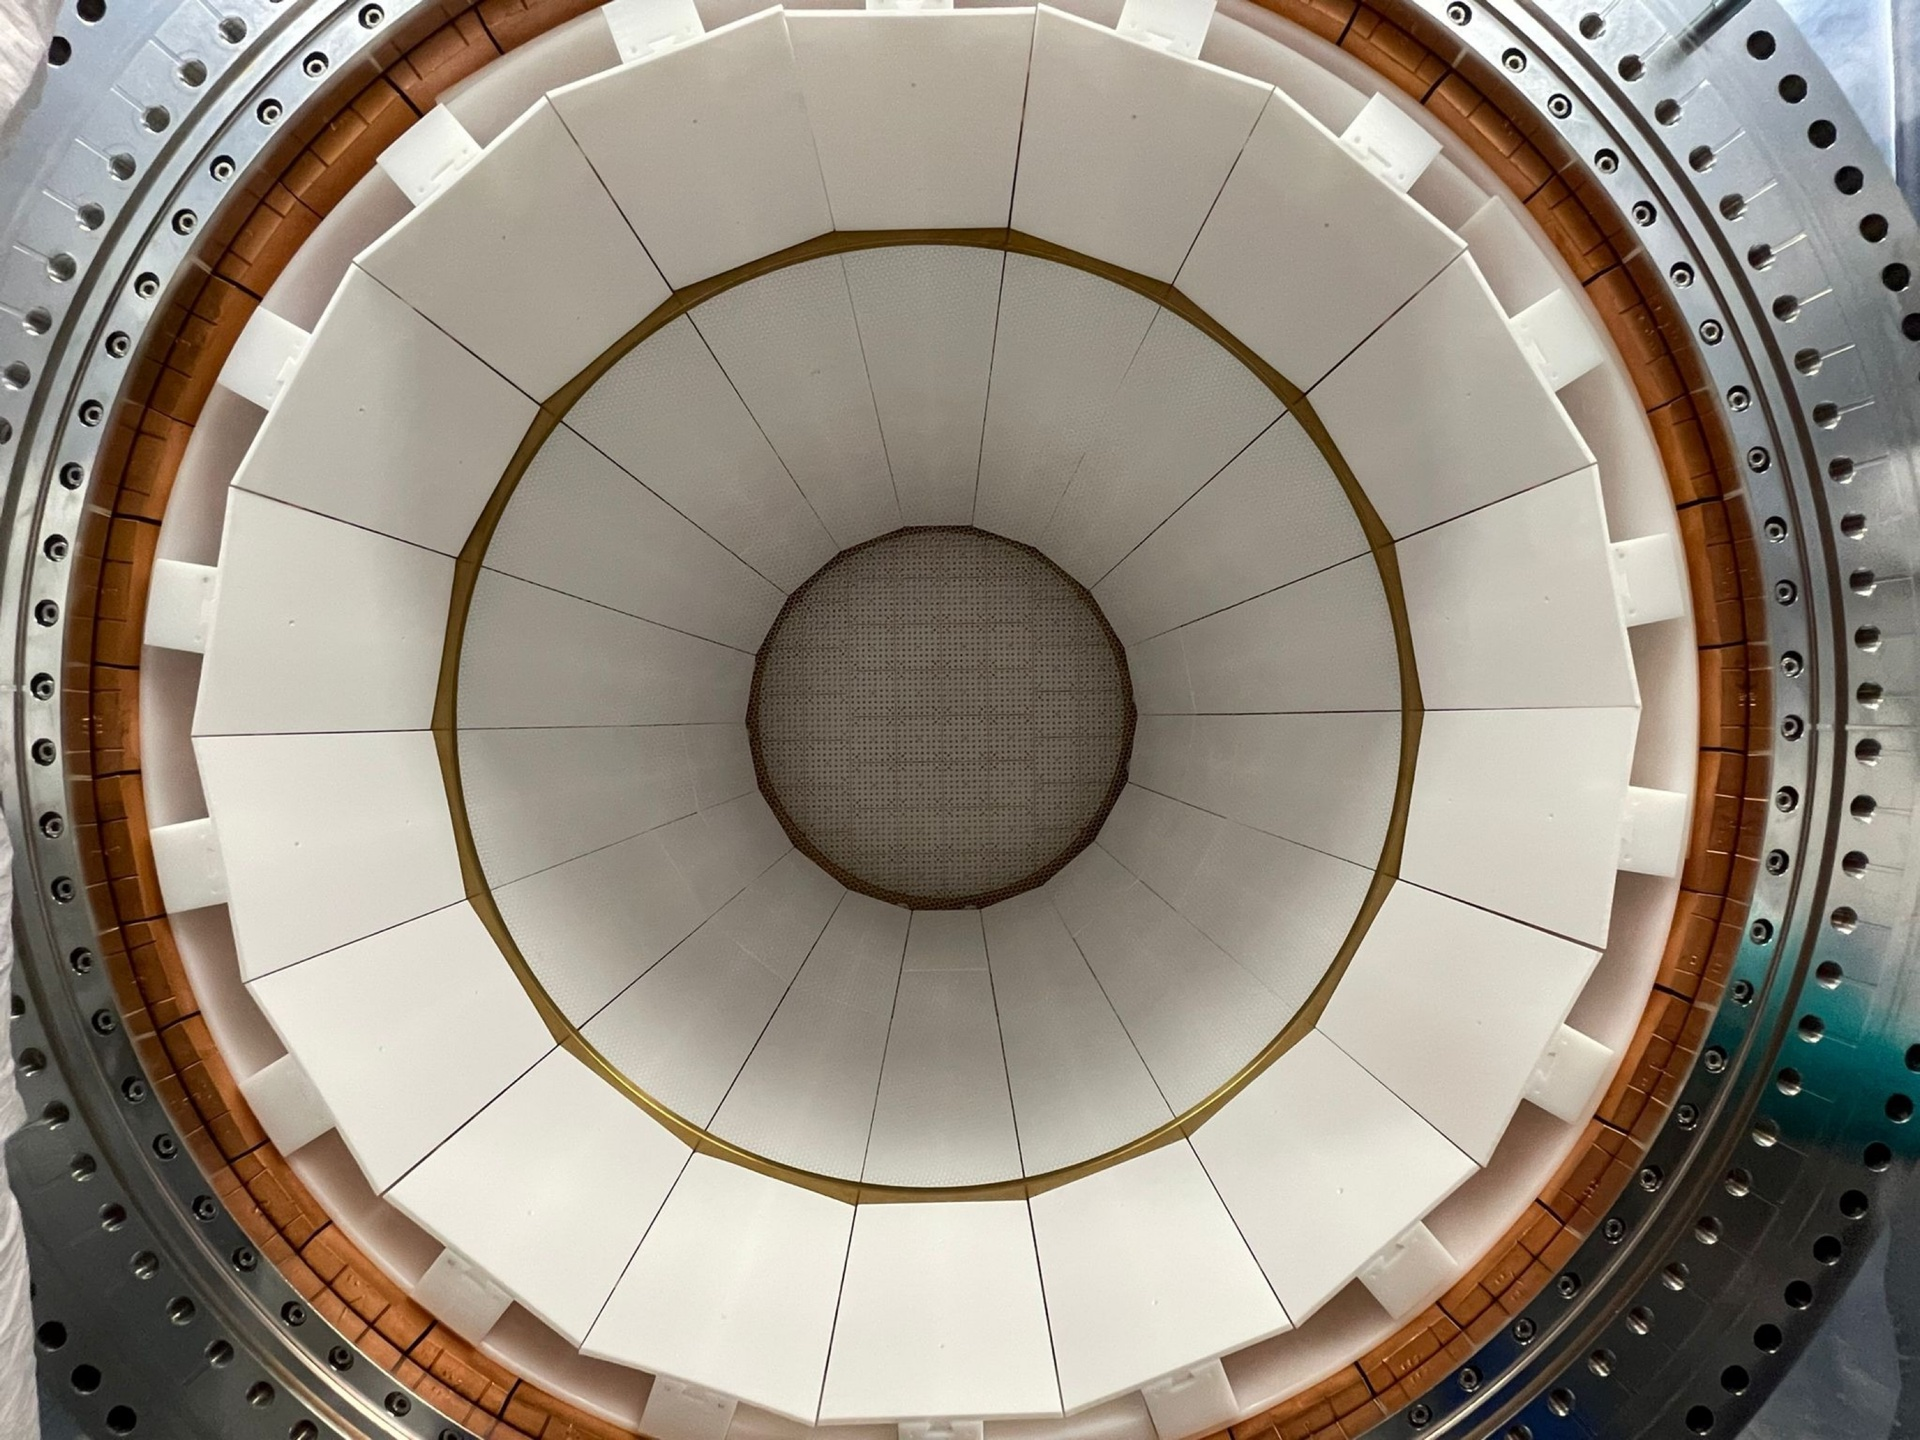
\includegraphics[width=\textwidth,height=0.75\textheight,keepaspectratio]{LightTube.jpg}

\end{columns}
\end{frame}



% =====================================================================
% 4. ¿PARA QUÉ SIRVE LA ANTIMATERIA?
% =====================================================================
%\begin{frame}{Tomografía por emisión de positrones (PET)}
%  \begin{columns}
%  \column{0.55\textwidth}
%    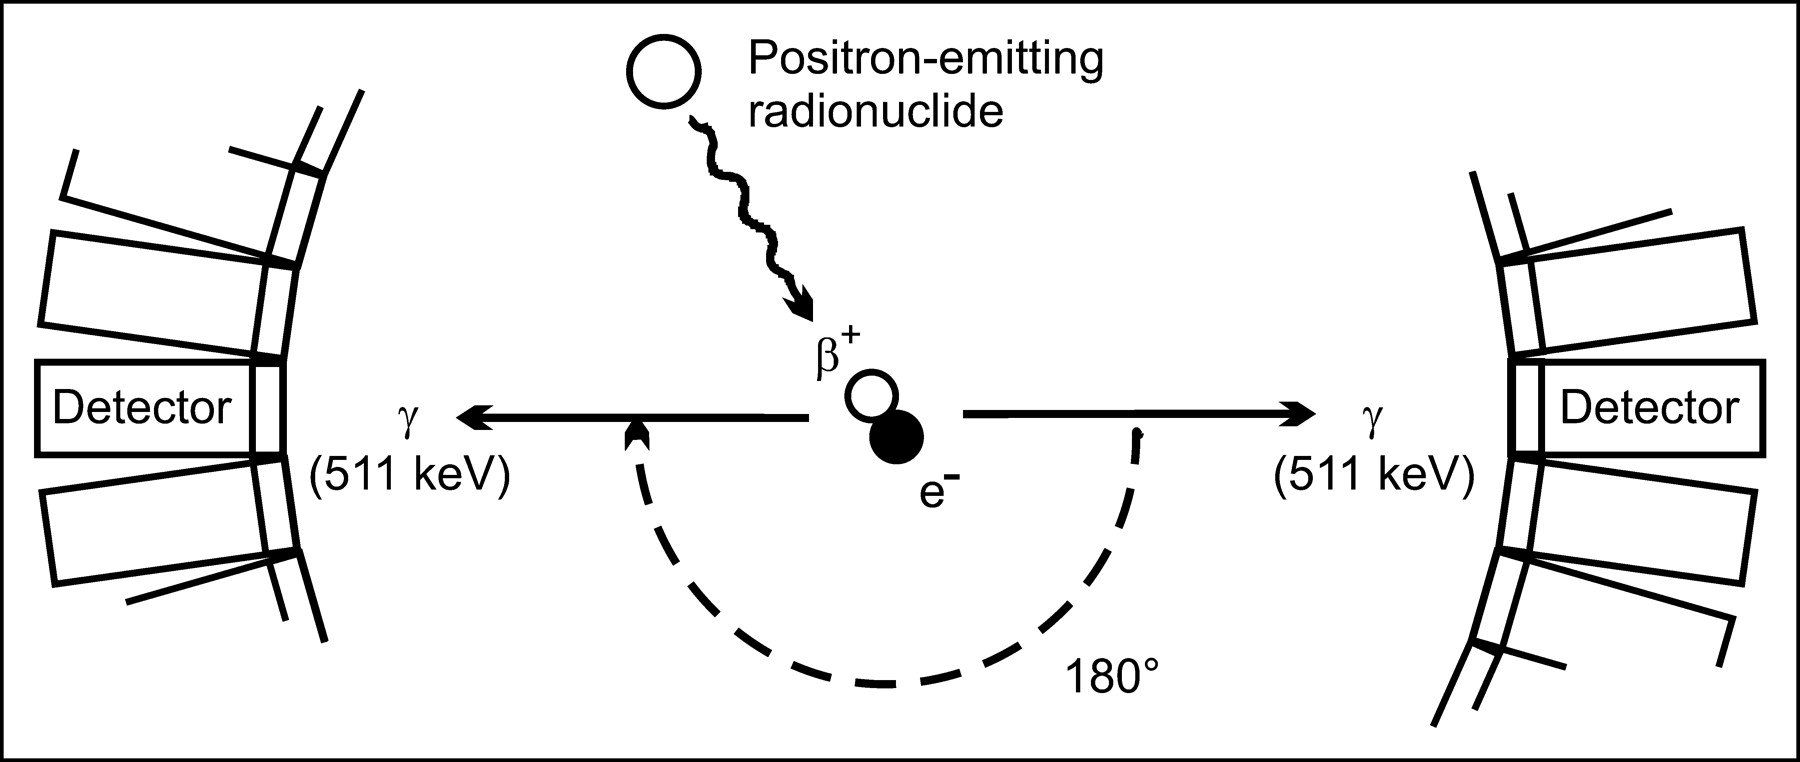
\includegraphics[width=\textwidth]{petPrinciple.png}
%  \column{0.45\textwidth}
%    Al paciente se le inyecta glucosa marcada con flúor-18, que emite
%    \textbf{positrones}.\\[1ex]
%    Cada positrón se aniquila con un electrón: dos fotones en direcciones
%    opuestas. Los mismos que vieron Reines y Cowan.\\[1ex]
%    Un anillo de detectores los ve en coincidencia. Muchas líneas cruzadas
%    forman la imagen.\\[1ex]
%    Los tumores consumen glucosa: se iluminan.
%  \end{columns}
%\end{frame}
%
%\begin{frame}{PET de cuerpo completo}
%  \begin{columns}
%  \column{0.45\textwidth}
%    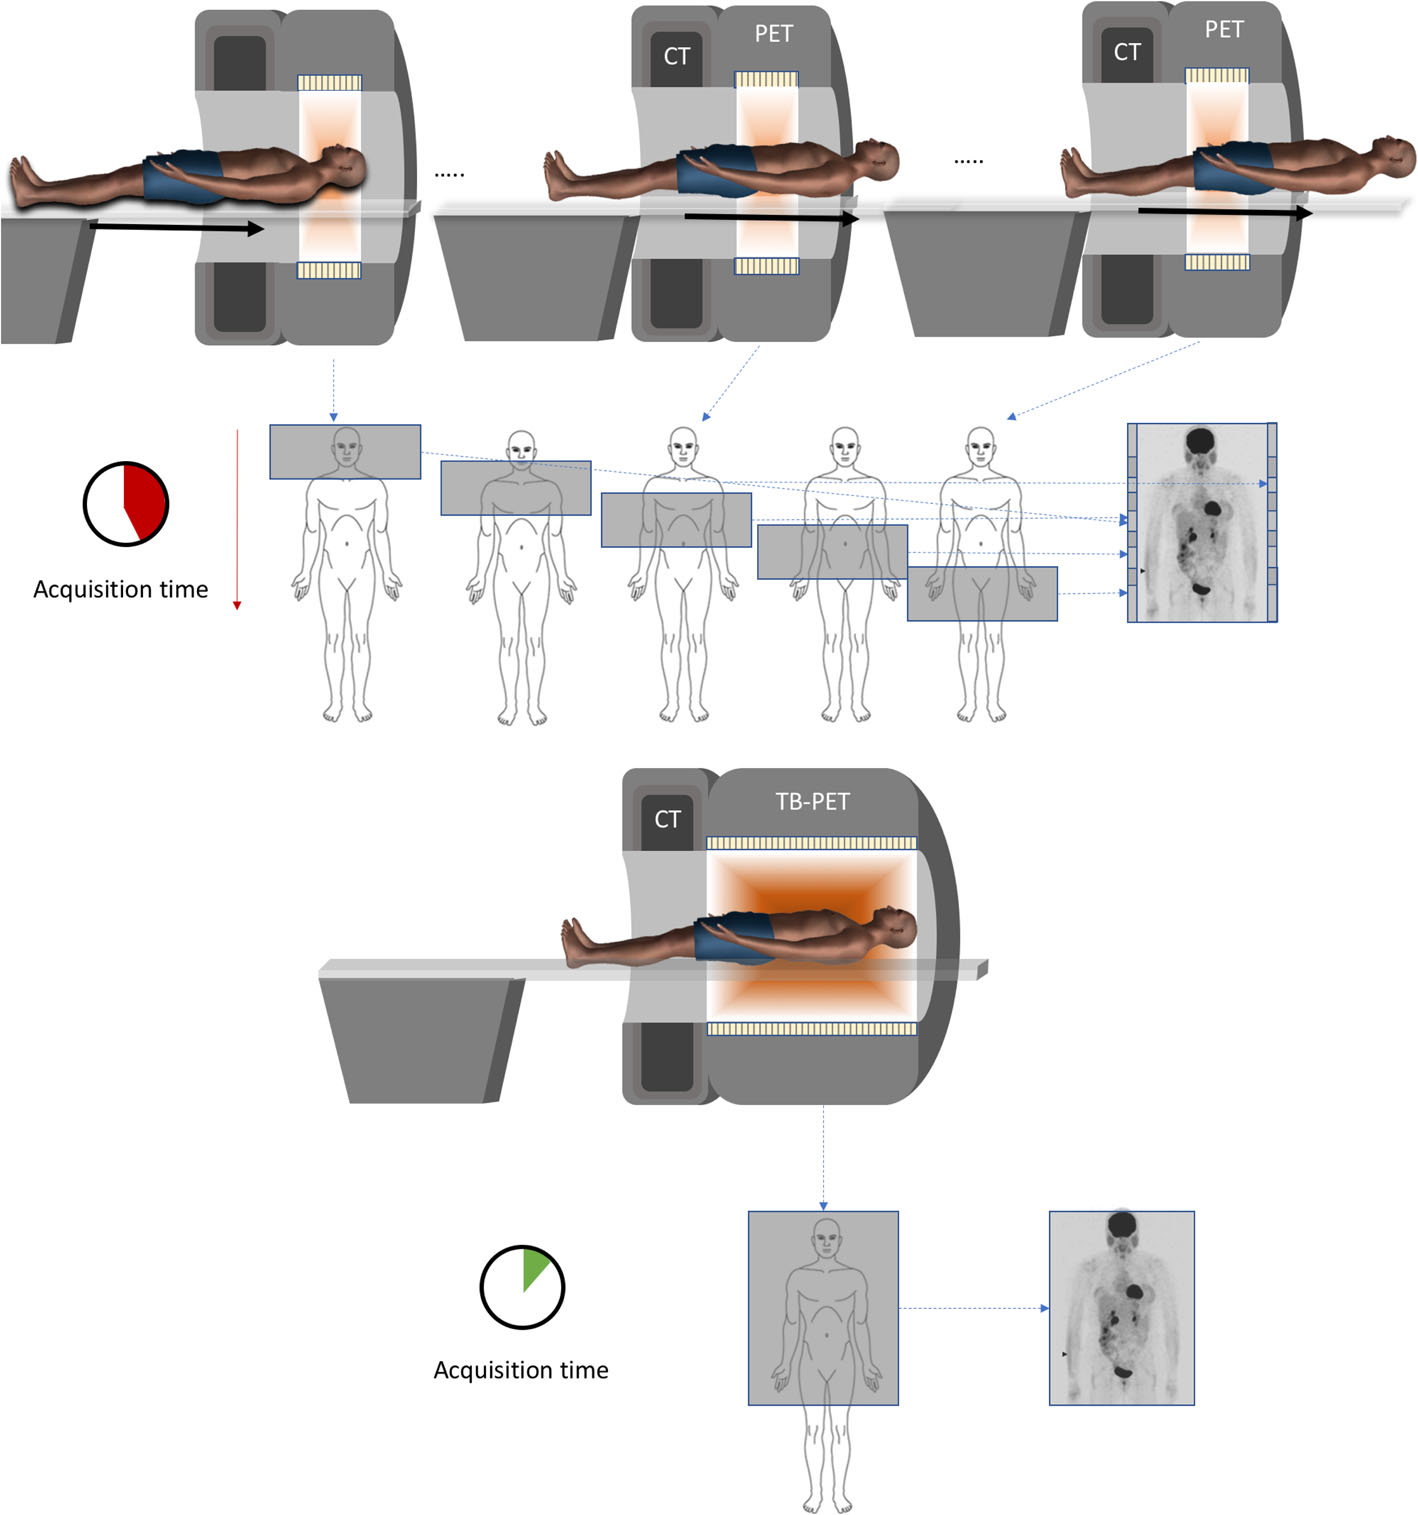
\includegraphics[width=\textwidth,height=0.75\textheight,keepaspectratio]{petWholeBody.png}
%  \column{0.55\textwidth}
%    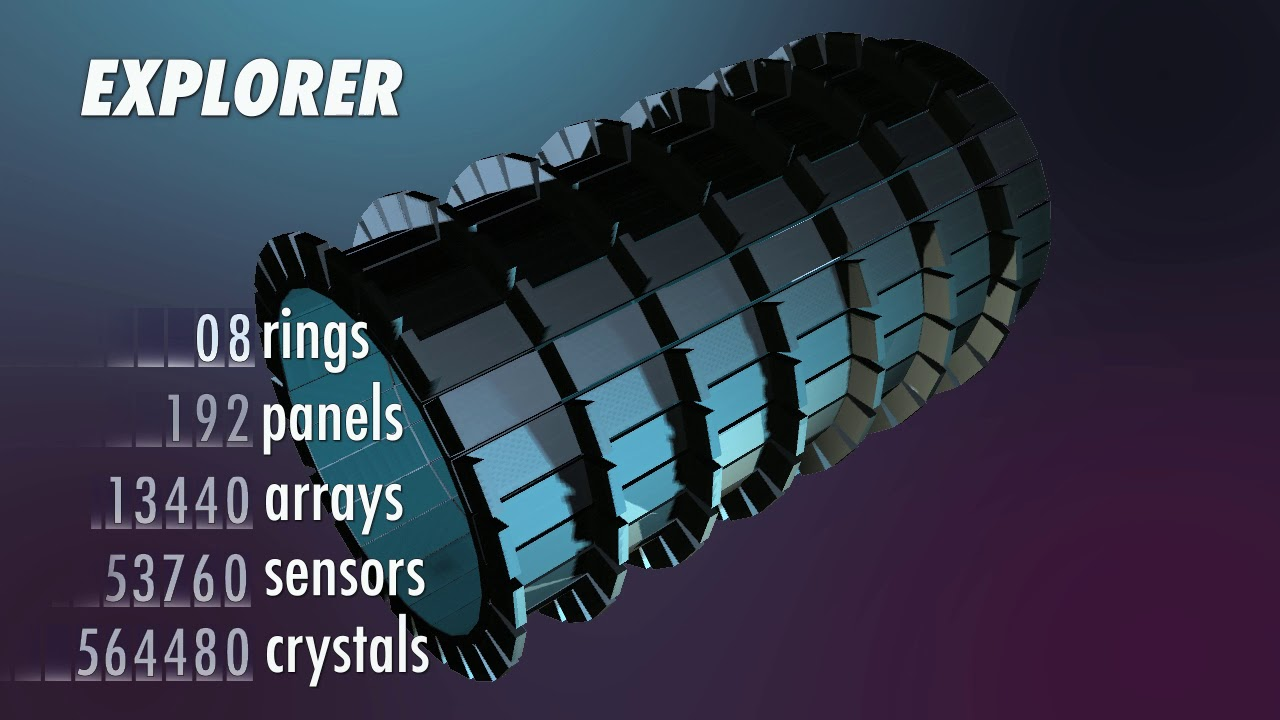
\includegraphics[width=\textwidth]{uExplorer.png}\\[1ex]
%    Un PET convencional cubre 20 cm. Uno de cuerpo entero lo ve todo a la
%    vez: cuarenta veces más sensible, menos dosis, menos tiempo.
%  \end{columns}
%\end{frame}
%
%\begin{frame}{PETALO: lo que hacemos en el DIPC}
%  \begin{columns}
%  \column{0.5\textwidth}
%    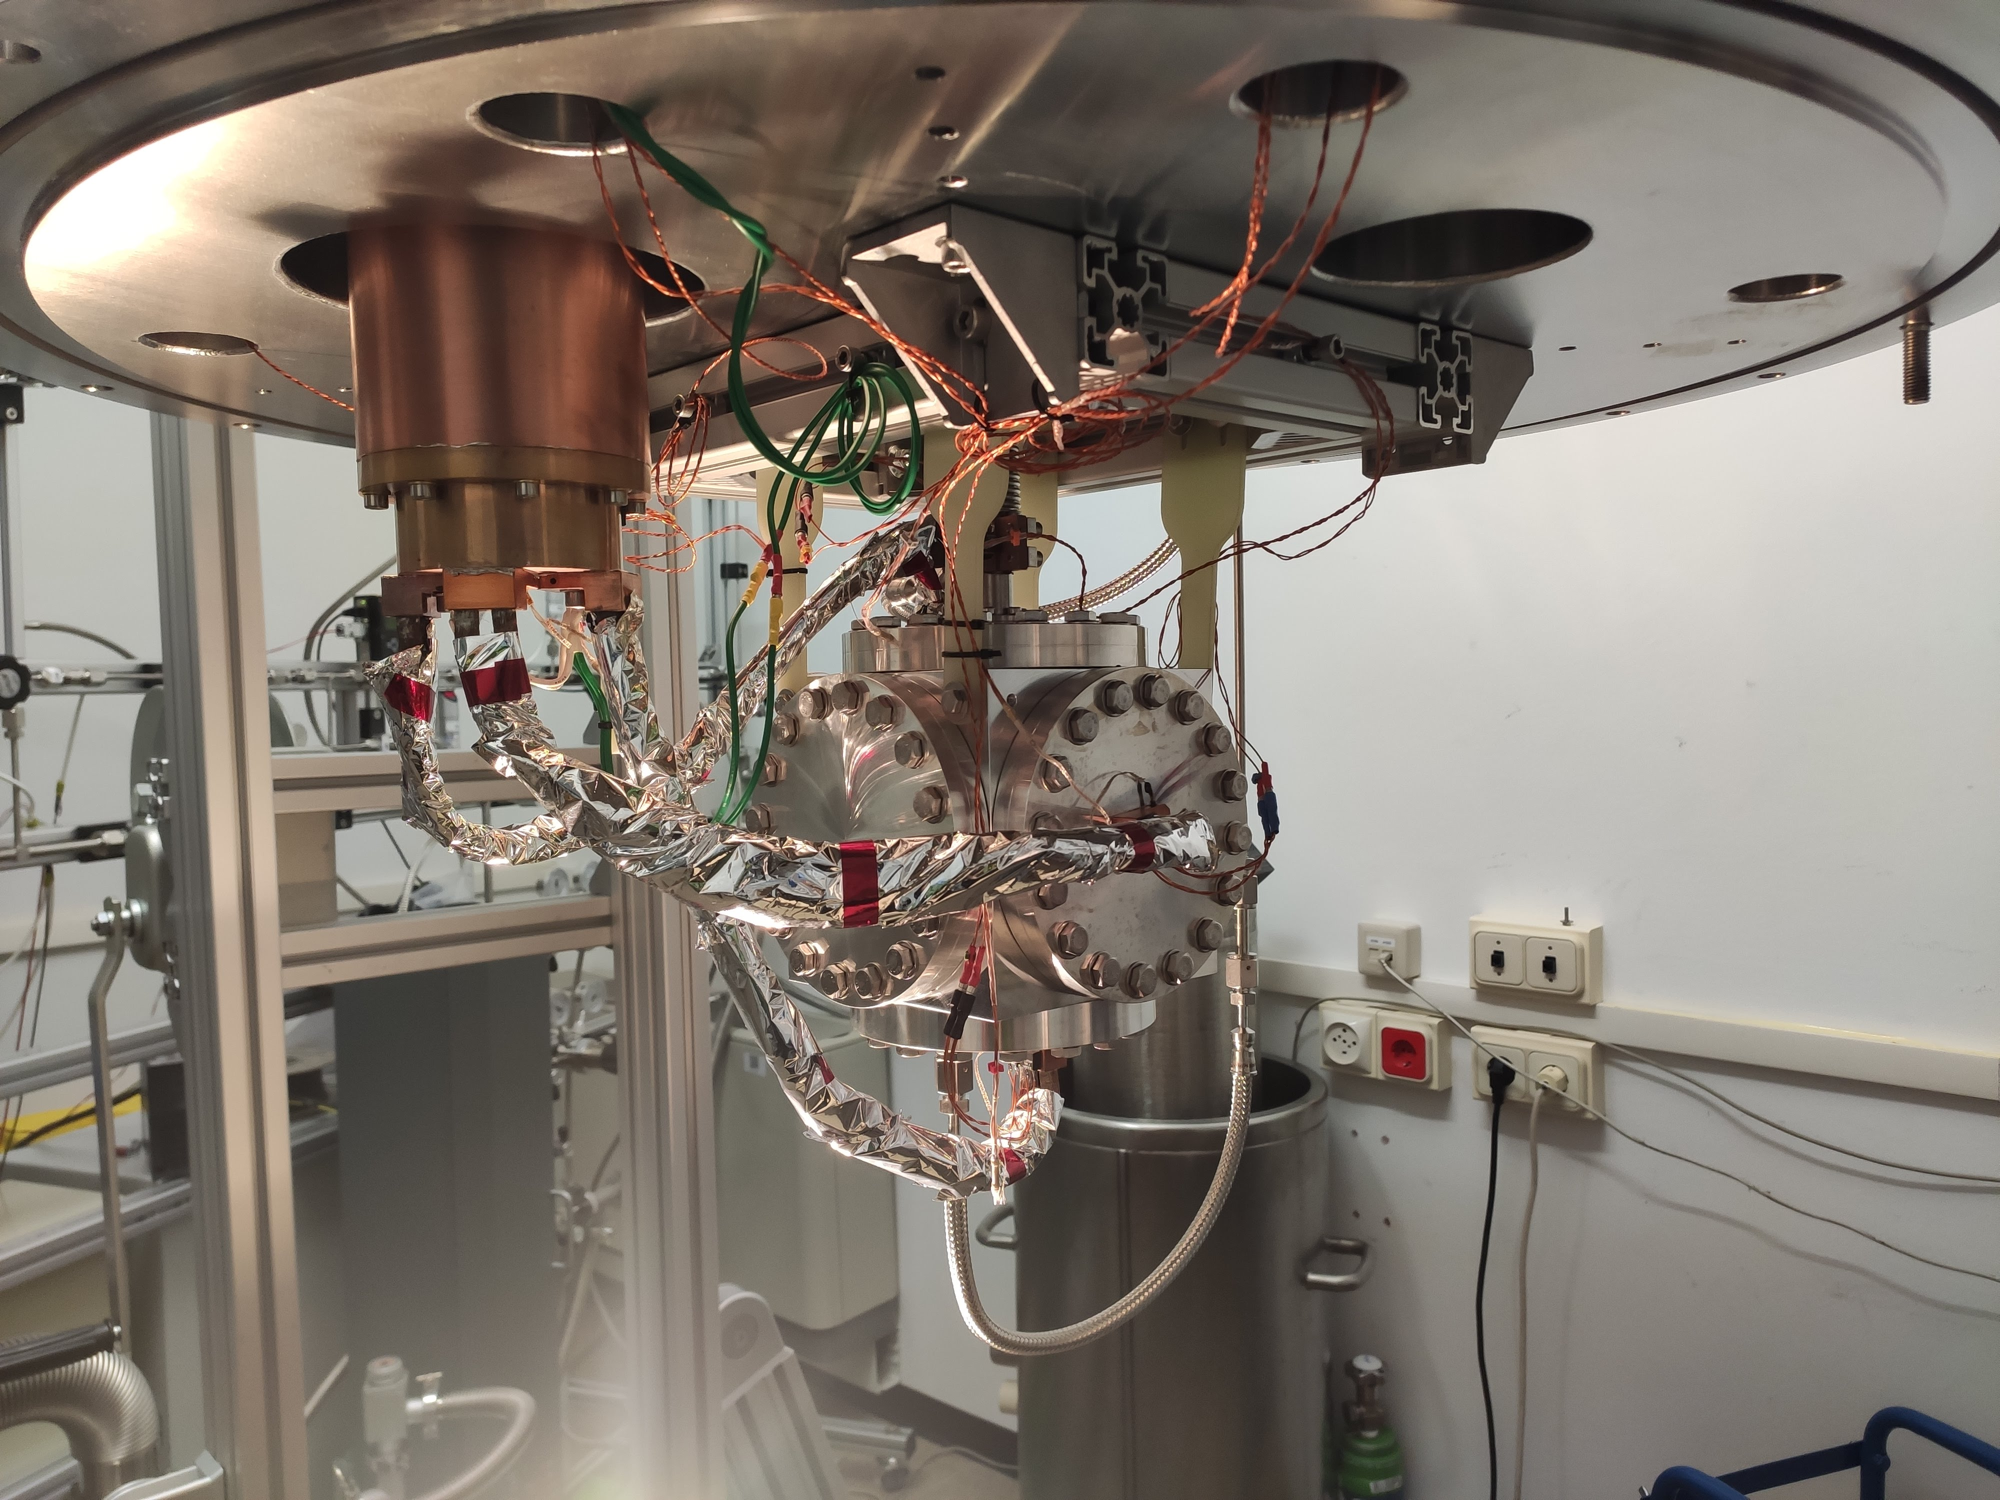
\includegraphics[width=\textwidth,height=0.7\textheight,keepaspectratio]{petitPrototypePhoto.png}
%  \column{0.5\textwidth}
%    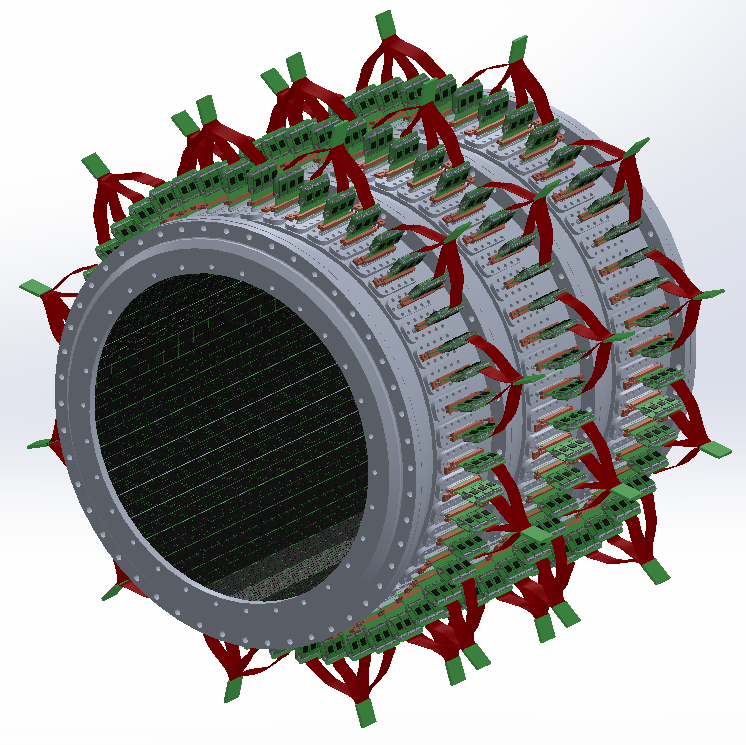
\includegraphics[width=\textwidth,height=0.5\textheight,keepaspectratio]{petaloWholeBodyCAD.png}\\[1ex]
%    Un PET de cuerpo completo de \textbf{xenón líquido}, en vez de cristales
%    de tierras raras. Prototipo ya construido.
%  \end{columns}
%\end{frame}
%
%\begin{frame}{PET y protonterapia en Donostia}
%  \pendiente[0.6\textheight]{Protonterapia: figuras y detalles, JJGC. Idea: verificar con PET dónde se detiene el haz de protones en el paciente.}
%\end{frame}
%
%% =====================================================================
%% 5. CIERRE
%% =====================================================================

%
%\begin{frame}
%  \frase{La sublime utilidad de la ciencia inútil}
%  \begin{center}
%  Pedro Miguel Echenique
%  \end{center}
%\end{frame}
%


\begin{frame}{Odiseas}
\begin{columns}
\column{0.50\textwidth}
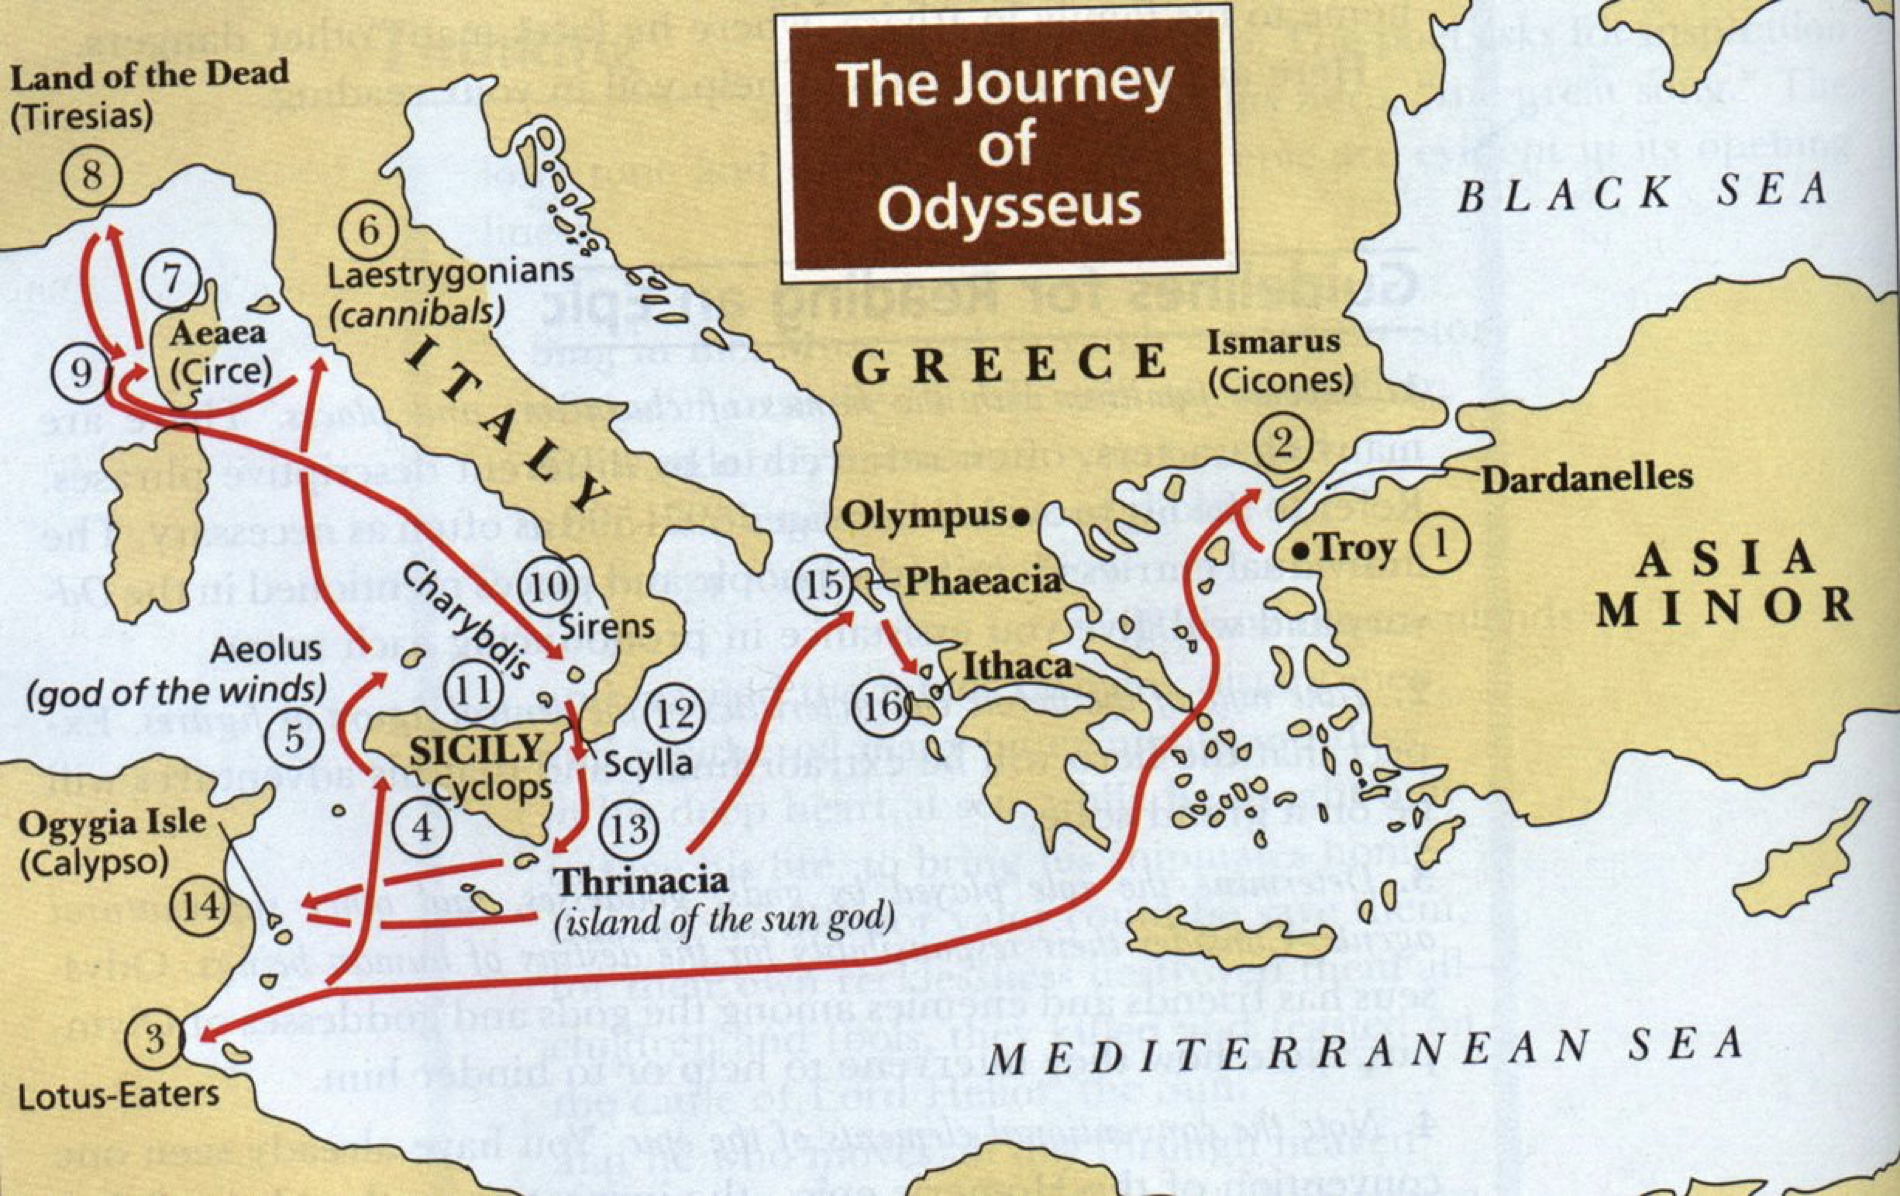
\includegraphics[width=\textwidth,height=0.55\textheight,keepaspectratio]{odyssey.png}

\column{0.50\textwidth}
$\bullet$~Los experimentos en física de neutrinos llevan mucho tiempo y los experimentos de $\beta\beta0\nu$ todavía más, tanto que solemos medirlos en <<viajes a Ítaca>>, es decir, en unidades de veinte años. 

$\bullet$~Los viajes que los experimentos realizan son parecidos a los de Ulises. Hay que pasar entre Escila y Caribdis (conseguir financiación, desarrollar una tecnología nueva), evitar que nos coman los cíclopes (competición con otros experimentos) y que nos hechicen poderosas ninfas (mantener la concentración durante décadas, sin despistarse con los cantos de sirena)\dots Todo para llegar a Ítaca, siempre sin saber si llegaremos.  

\end{columns}
\end{frame}

\begin{frame}{Rilke}
  \begin{columns}[T]
  \column{0.48\textwidth}
    \begin{cita}
    Sie nährten es mit keinem Korn,\\
    nur immer mit der Möglichkeit, es sei.
    \end{cita}
  \column{0.48\textwidth}
    \begin{cita}
    No lo alimentaron con grano,\\
    sino con la convicción de que podría existir. 
    \end{cita}
  \end{columns}
  \vspace{1cm}
  \begin{center}
 % {\large\color{uwopurple} Es la fe en la ciencia la que hace real al unicornio.}
  \end{center}
\end{frame}

\end{document}
